% !TEX TS-program = latexmk

\documentclass[12pt,twoside,spanish]{book}

% Verificacion de sintaxis sin producir salida:
% descomentar la segunda linea para verificar
% sintaxis sin producir salida.
\usepackage{syntonly}
% \syntaxonly

% Palabras clave en distintos idiomas
\usepackage[activeacute]{babel}

% Patrones para division en silabas
\hyphenation{par-ti-cu-lar}

% Inclusion de imagenes
\usepackage{graphicx}

% Codificacion de simbolos
\usepackage[T1]{fontenc}
\usepackage[applemac]{inputenc}

% Fuentes y simbolos adicionales
\usepackage{amsfonts}
\usepackage{amsmath}
\usepackage{amssymb}
\usepackage{mathrsfs}

% Colores
\usepackage[table]{xcolor}

\definecolor{verdeOscuro}{rgb}{0,0.6,0}
\definecolor{verdeAzulado}{RGB}{27, 154, 170}
\definecolor{gris}{rgb}{0.5,0.5,0.5}
\definecolor{malva}{rgb}{0.58,0,0.82}
\definecolor{grisClaro}{rgb}{0.92,0.92,0.92}
\definecolor{grisOscuro}{RGB}{87, 90, 102}
\definecolor{amarilloOscuro}{RGB}{216, 175, 57}
\definecolor{azulMetal}{RGB}{39, 139, 154}
\definecolor{salmon}{RGB}{222, 120, 98}
\definecolor{rosa}{RGB}{231, 91, 100}
\definecolor{azulOscuro}{RGB}{21, 92, 117}
\definecolor{baige}{RGB}{154, 131, 113}
\definecolor{verde}{RGB}{120, 188, 97}
\definecolor{fushia}{RGB}{239, 71, 111}
\definecolor{naranja}{RGB}{249, 132, 0}
\definecolor{menta}{RGB}{6, 214, 160}
\definecolor{cereza}{RGB}{181, 10, 42}
\definecolor{GverdePasto}{RGB}{	115, 143, 55}
\definecolor{crema}{RGB}{238,216,194}
\definecolor{oro}{RGB}{216, 175, 57}
\definecolor{crema}{RGB}{238,216,194}
\definecolor{amarillo}{RGB}{230,194,41}
\definecolor{azulClaro}{RGB}{127,209,185}
\definecolor{lila}{RGB}{163,121,201}
\definecolor{coral}{RGB}{247,142,105}
%\definecolor{verde}{RGB}{104,163,87}
\definecolor{azulCielo}{RGB}{0,178,202}
\definecolor{morado}{RGB}{152,95,153}
\definecolor{azulFuerte}{RGB}{19,84,102}
\definecolor{vino}{RGB}{154,3,30}


% Vinculos
\usepackage{hyperref}
\hypersetup{
  colorlinks,
  urlcolor={malva}
}

% Codigo
\usepackage{listings}
\lstset{
  language=[LaTeX]TeX,
  aboveskip=3mm,
  belowskip=3mm,
  showstringspaces=false,
  columns=flexible,
  basicstyle={\small\ttfamily},
  numbers=none,
  extendedchars=true,
  numberstyle=\tiny\color{gris},
  keywordstyle=\color{blue},
  commentstyle=\color{verdeOscuro},
  stringstyle=\color{malva},
  breaklines=true,
  breakatwhitespace=true,
  tabsize=3,
  backgroundcolor=\color{grisClaro},
  moretexcs={color},
}


% Algoritmos
%\usepackage[ruled,lined,linesnumbered,commentsnumbered]{algorithm2e}

%\usepackage[all]{xy}

% Generacion de dibujos con TeX
\usepackage{tikz}
\usetikzlibrary{arrows,shapes,matrix,decorations,calc,positioning}
\tikzstyle{arc}   =[->,shorten <=3pt, shorten >=3pt,
                   >=stealth, line width=1.1pt]
\tikzstyle{edge}  =[shorten <=2pt, shorten >=2pt,
                    >=stealth, line width=1.1pt]
\tikzstyle{wedge}  =[shorten <=2pt, shorten >=2pt,
                    >=stealth, line width=1.3pt]
\tikzstyle{nedge}  =[shorten <=2pt, shorten >=2pt,
                    >=stealth, line width=0.7pt]
\tikzstyle{myloop}=[style={},shorten <=1pt, shorten >=1pt,
                    >=stealth, line width=1.1pt, loop]
\tikzstyle{vertex}=[circle, draw, minimum size=6pt,
                    line width=0.75pt, inner sep=0pt,
                    outer sep=0pt]
 \tikzstyle{wvertex}=[circle, draw, minimum size=6pt,
                    line width=0.75pt, inner sep=0.5pt,
                    outer sep=0pt]
\tikzstyle{bvertex}=[circle, draw, minimum size=7pt,
                    line width=0.75pt, inner sep=0pt,
                    outer sep=0pt]
\tikzstyle{svertex}=[circle, draw, minimum size=4.5pt,
                    line width=0.75pt, inner sep=0pt,
                    outer sep=0pt]
\tikzstyle{Bvertex}=[circle, draw, minimum size=43pt,
                    line width=0.75pt, inner sep=0pt,
                    outer sep=0pt]
\tikzstyle{cvertex}=[circle, draw=grisOscuro!75, minimum size=6pt,
                    line width=0.75pt, inner sep=0pt,
                    outer sep=0pt]
\tikzstyle{avertex}=[circle, draw=azulCielo, minimum size=7.5pt,
                    line width=1.5pt, inner sep=0pt,
                    outer sep=0pt]
\tikzstyle{coralvertex}=[circle, draw=coral, minimum size=7.5pt,
                    line width=1.8pt, inner sep=0pt,
                    outer sep=0pt]
\tikzstyle{amarvertex}=[circle, draw=amarillo, minimum size=7.5pt,
                    line width=1.8pt, inner sep=0pt,
                    outer sep=0pt]
\tikzstyle{mvertex}=[circle, draw=morado, minimum size=7.5pt,
                    line width=1.8pt, inner sep=0pt,
                    outer sep=0pt]


% Ajuste de parametros en la pagina
\usepackage{geometry}

% Ubicacion precisa de floats
\usepackage{float}

% Manejo de encabezados
\usepackage{fancyhdr}

% Estilo de encabezados
\pagestyle{fancy}
\renewcommand{\chaptermark}[1]{\markboth{#1}{}}
\renewcommand{\sectionmark}[1]{\markright{\thesection\ #1}}
\fancyhf{}
\fancyhead[LE,RO]{\textsc{\bfseries\nouppercase\thepage}}
\fancyhead[LO]{\textsc{\bfseries\nouppercase\rightmark}}
\fancyhead[RE]{\textsc{\bfseries\nouppercase\leftmark}}
\renewcommand{\headrulewidth}{0.5pt}
\renewcommand{\footrulewidth}{0pt}
\addtolength{\headheight}{3pt}
\fancypagestyle{plain}{
  \fancyhead{}
  \renewcommand{\headrulewidth}{0pt}
}

% Delimitadores para terminar las demostraciones
\newcommand{\blackqed}{\hfill$\blacksquare$}
\newcommand{\whiteqed}{\hfill$\square$}
\newcounter{proofcount}

% Generacion de tabla de contenidos
\usepackage{makeidx}
\makeindex

% Ambientes de teorema y demostracion
\usepackage{amsthm}

% Referencias con nombres automaticos
\usepackage{cleveref}

% Definiciones de nuevos ambientes
\newtheorem{teorema}{Teorema}[section]
\newtheorem{lema}[teorema]{Lema}
\newtheorem{proposicion}[teorema]{Proposici\'on}
\newtheorem{corolario}[teorema]{Corolario}

\theoremstyle{definition}
\newtheorem{definicion}[teorema]{Definici\'on}

% Nombres para cleveref
\crefname{teorema}{el Teorema}{los Teoremas}
\crefname{lema}{el Lema}{los Lemas}
\crefname{proposicion}{la Proposici\'on}{las Proposiciones}
\crefname{corolario}{el Corolario}{los Corolarios}
\crefname{algorithm}{el Algoritmo}{los Algoritmos}
\crefname{section}{la Secci\'on}{las Secciones}
\crefname{figure}{la Figura}{las Figuras}

% Redefinicion para que las demostraciones terminen con cuadrito negro
\renewenvironment{proof}[1][\proofname.]{\par
\ifnum%
\theproofcount>0 \pushQED{\whiteqed} \else \pushQED{\blackqed} \fi%
\refstepcounter{proofcount}
%
\normalfont%\topsep6\p@\@plus6\p@\relax
\trivlist%
\item[\hskip\labelsep%
\itshape%
\textbf{\textit{#1}}]\ignorespaces%
}{%
\addtocounter{proofcount}{-1}
\popQED\endtrivlist%
}

% Macros
% Abreviatura para fuentes true type
\newcommand{\ttt}[1]{%
\texttt{#1}%
}

\newcommand{\indice}[1]{%
\textbf{#1}\index{#1}%
}

\newcommand{\indiceSub}[2]{%
\textbf{#2}\index{#1!#2}%
}

\begin{document}

\frontmatter

%%
%% Portada creada por la Facultad de Ciencias
%%

%%
%% Esqueleto para la portada de las tesis para
%% la Facultad de Ciencias de la UNAM
%%


%%%%%%%%%%%%%%%%%%%%%%%%%%%%%%%%%%%%%%%%%%%%%%%%%%%%%%%
%% Comandos para la portada

\newcommand{\titulo}[1]{\def\eltitulo{#1}}
%* la carrera corresponde al tí­tulo otorgado -Matemático-
%* NO AL NOMBRE DE LA CARRERA -Matemáticas- --RRP
\newcommand{\carrera}[1]{\def\lacarrera{#1}}
\newcommand{\nombre}[1]{\def\elnombre{#1}}      %* Del alumno
\newcommand{\director}[1]{\def\eldirector{#1}}  %* De tesis
\newcommand{\fecha}[1]{\def\lafecha{#1}}

%% Llene los siguientes datos (use MAYÚSCULAS)
%% Estos datos aparecerán en la portada y los encabezados
\titulo{UNA INTRODUCCI\'ON A LAS GR\'AFICAS DE FICHAS}
\nombre{\uppercase{ADRICA MERINO S\'ANCHEZ}}
\carrera{MATEM\'ATICO}
\director{\uppercase{C\'ESAR HERN\'ANDEZ CRUZ}}
\fecha{2024}


\thispagestyle{empty}

%% Barra izquierda - Escudos
\hskip-1.5cm
\begin{minipage}[c][10cm][s]{3cm}
  \begin{center}
    
\includegraphics[height=2.6cm]{escudo-unam.pdf}\\[10pt]
    \hskip2pt\vrule width2pt height13cm\hskip1mm
    \vrule width1pt height13cm\\[10pt]
    
\includegraphics[height=2.6cm]{escudo-ciencias.pdf}
  \end{center}
\end{minipage}\quad
%% Barra derecha - Tí­tulos
\begin{minipage}[c][9.5cm][s]{10cm}
  \begin{center}
    % Barra superior
    {\large \scshape Universidad Nacional Aut\'onoma de M\'exico}
    \vspace{.3cm}
    \hrule height2pt
    \vspace{.1cm}
    \hrule height1pt
    \vspace{.3cm}
    {\scshape Facultad de Ciencias}

    % Titulo del trabajo
    \vspace{3cm}

    {\Large \eltitulo}

    \vspace{3cm}

    % Tipo de trabajo
    \makebox[8cm][s]{\Huge T E S I S}\\[8pt]
    QUE PARA OBTENER EL T\'ITULO DE:\\[3pt]
    \mbox{}\lacarrera\\[13pt]
    PRESENTA:\\[3pt]
    \elnombre

    \vspace{2cm}

    {\small DIRECTOR DE TESIS:\\ \eldirector}

    \vspace{2cm}

    \lafecha

  \end{center}
\end{minipage}

{\small
\begin{quote}
\begin{tabular}{lll}
1.Datos del alumno          & {}                                          \\
Apellido paterno            & Merino                                     \\
Apellido materno            & S\'anchez                                     \\
Nombre (s)                   & Adrica                                     \\
Tel\'efono                  &                              \\
Universidad                 & Universidad Nacional Aut\'onoma de M\'exico \\
Facultad o escuela          & Facultad de Ciencias                        \\
Carrera                     & Matem\'aticas                                     \\
N\'umero de cuenta          & 41607030-7                                   \\
{}                          & {}                                          \\
2. Datos del tutor          & {}                                          \\
Grado                       & Dr.                                         \\
Nombre (s)                   & C\'esar                                     \\
Apellido paterno            & Hern\'andez                                 \\
Apellido materno            & Cruz                                        \\
{}                          & {}                                          \\
3. Datos del sinodal 1      & {}                                          \\
Grado                       & Dra.                                        \\
Nombre (s)                   & Rita Esther                                     \\
Apellido paterno            & Zuazua                                     \\
Apellido materno            & Vega                                     \\
{}                          & {}                                          \\
4. Datos del sinodal 2      & {}                                          \\
Grado                       & Dra.                                          \\
Nombre (s)                   & Ana Paulina                                     \\
Apellido paterno            & Figueroa                                     \\
Apellido materno            & Guti\'errez                                 \\
{}                          & {}                                          \\
5. Datos del sinodal 3      & {}                                          \\
Grado                       & Dr.                                        \\
Nombre (s)                   & Fernando Esteban                           \\
Apellido paterno            & Contreras                                     \\
Apellido materno            & Mendoza                                     \\
{}                          & {}                                          \\
6. Datos del sinodal 4      & {}                                          \\
Grado                       & Dr.                                          \\
Nombre (s)                   & Germ\'an                                     \\
Apellido paterno            & Ben\'itez                                     \\
Apellido materno            & Bobadilla                                     \\
{}                          & {}                                          \\
7.Datos del trabajo escrito & {}                                          \\
T\'itulo                    & Una introducci\'on a las gr\'aficas de fichas  \\
N\'umero de p\'aginas       & 66 p.                                       \\
A\~no                       & 2024                                        \\
\end{tabular}
\end{quote}
}

\chapter*{Agradecimientos}
\addcontentsline{toc}{chapter}{Agradecimientos}


\textit{A mi asesor, C\'esar, creer en mi, ense\~{n}arme tanto, darme su tiempo
y apoyo durante todo este proceso; por ser una ispiraci\'on, tanto como profesor
como persona.}\\

\textit{A mi mam\'a, Rosana, por siempre estar lista para apoyarme, darme
consejos y ayudarme a encontrar soluciones;  por siempre guiarme con una
sonrisa. A mi pap\'a, Lucas,  por su humor, sus bailes y su optimismo. Gracias
por ayudarme a enamorarme de las matem\'aticas. Gracias a ambos por todo su
apoyo, cari\~{n}o y amor incondicional; por cacharme cuando me caigo y
aplaudirme cuando me levanto.}\\

\textit{A mi hermano, Tabar\'e, por ser la compa\~{n}ia constante en todas mis
etapas, incluyendo la carrera; por entenderme como s\'olo \'el puede y por las
ense\~{n}anzas que me ha dado toda mi vida.}\\

\textit{A Nancy, por ser un rayo de luz y de risa al cual siempre puedo
regresar; por las platicas, los chismes y la paciencia para ver todas mis
fotos.}\\

\textit{A Rach, por todo el apoyo, la compa\~{n}ia y gu\'ia en este periodo, al
igual que las risas, las pl\'aticas y las discuciones sobre el futuro. A Xime,
por las pl\'aticas y las desveladas en los finales de semestres. Gracias a las
dos por haber sido ek lugar al cual poder regresar, desahogarme y recargarme de
energ\'ia.} \\

\textit{A la Dracs, por su cari\~{n}o, apapachos, su amor y su compa\~{n}\'ia
constante; por ser mi despertador y mi desestr\'es. Gracias por haberme
elegido. A la Mixtli, por acompa\~{n}arme al estudiar para los ex\'amenes, la
raz\'on para darme un respiro y por su alegr\'ia y amor, que me brind\'o desde
el primer momento.}\\ 

\textit{A mi familia del Cineclub de Ciencias, por el espacio tan acojedor  y
donde ser yo misma, con personas hermosas e invaluables que hicieron de mis
a\~{n}os en la facultad una de las mejores etapas de mi vida.}\\

\textit{A Mich, Zare y Eliel, por haberme dado un lugar al cual pertenecer desde
el primer semestre, as\'i como su amistad y cari\~{n}o.}\\

\textit{A Carlos, por haber sido mi fuerza y motivaci\'on para acabar este
trabajo. Gracias por tu compa\~{n}ia y apoyo en los momentos que los m\'as
necesitaba.}\\

\textit{A Zyanya, por todas las pl\'aticas de chismes y de la vida, muchs veces
disfrazadas de seciones de estudio. Gracias por tu escucha y apoyo siempre.}\\

\textit{A Renata, por todas nuestras salidas, platicas, chismes y risas; por
darme constante apoyo y motivaci\'on.}\\

\textit{A Javi, por las grandes platicas y la ayuda para lograr este trabajo.}\\

\textit{A B\'arbara, por ser un gran apoyo y gu\'ia; por ense\~{n}arme la fuerza
que tengo para lograr las cosas.}\\
\tableofcontents


\mainmatter%

%\chapter{Introducci\'on}
\label{sec:intro}

Este documento tiene algunos ejemplos m\'inimos de caracter\'isticas que se
suelen utilizar en tesis de las licenciaturas en matem\'aticas y ciencias de la
computaci\'on, en particular en el \'area de teor\'ia de gr\'aficas (el \'area
de trabajo del autor).

Se exhorta al usuario a leer la
\href{https://tobi.oetiker.ch/lshort/lshort.pdf}{Not So Short Inroduction to
\LaTeX}.   Aunque realmente no es un documento muy largo, para quienes nunca han
usado \LaTeX{} es posible que las partes t\'ecnicas no tengan sentido.   En este
caso, es recomendable leer los dos primeros cap\'itulos, y regresar al resto del
documento para hacer consultas, o cuando se tenga algo de experiencia y se
desee mejorar como usuario.   En particular, antes de intentar cambiar el tipo
de letra, o el tama\~no de los m\'argenes, considere la siguiente observaci\'on
que aparece en el documento antes mencionado:
\begin{quote}
  Typographical design  is  a  craft.   Unskilled  authors  often  commit
  seriousformatting errors  by  assuming  that  book  design  is  mostly  a
  question of aesthetics---``If a document looks good artistically, it is well
  designed.'' But as a document has to be read and not hung up in a picture
  gallery, the readability and understandability is of much greater importance
  than the beautiful look of it.
\end{quote}

Idealmente, el lector obtuvo esta plantilla mediante
\href{https://github.com/Japodrilo/template-tesis}{este repositorio}. De no ser
as\'i, se le invita a visitarlo, y a usar las bondades del control de versiones
que el uso de \href{https://git-scm.com/}{Git} otorga (en particular cuando se
utiliza en conjunto con alguna plataforma para albergar sus repositorios
remotamente\footnote{Los alumnos de la Facultad de Ciencias de la UNAM tienen
acceso al \href{https://education.github.com/pack}{GitHub Student Developer
Pack} con su cuenta \ttt{@ciencias.unam.mx}.}).


\section{C\'omo usar esta plantilla}
\label{sec:howto}

Esta plantilla se dise\~n\'o como una ayuda para aquellos usuarios que ya
est\'an familiarizados con \LaTeX, pero nunca han desarrollado un proyecto
``grande'' (m\'as all\'a de tareas o reportes finales de proyectos).   Siguiendo
las instrucciones encontradas en el archivo \ttt{README.md}, lo m\'as probable
es que hayan creado un nuevo repositorio a partir del ``template repository''
que contiene este proyecto.   En primer lugar, verifique que el proyecto compile
adecuadamente; el proyecto deber\'ia de compilar sin errores ni advertencias. Es
posible que la primera vez que se compila, su manejador de paquetes actualice
varios de \'estos, lo que puede llevar un tiempo.   En caso de tener errores, es
posible que \'estos se deban a la falta de algunos paquetes, y a que su
manejador de paquetes no los instala autom\'aticamente;  instalar los paquetes
faltantes manualmente deber\'ia de resolver todos los problemas.

La estructura de este proyecto es sencilla.   Hay un archivo central,
\ttt{tesis.tex}, que contiene el pre\'ambulo del documento, y donde se incluyen
todos los paquetes y definiciones necesarias.   El c\'odigo est\'a comentado,
explicando de forma m\'inima para qu\'e sirve cada comando; se recomienda que al
modificarlo se mantenga un estilo semejante para no causarle problemas
innecesarios a su yo del futuro.   Todos los contenidos se encuentran en otros
archivos dentro del mismo directorio, que son llamados desde \ttt{tesis.tex}
mediante el comando \ttt{\textbackslash{include}}.   De esta forma se
incluyen la car\'atula, la hoja de datos, los cap\'itulos que forman parte de la
tesis, la bibliograf\'ia, etc.   Por otro lado, \LaTeX~ genera (casi)
autom\'aticamente el \'indice y el \'indice alfab\'etico, pero hay que agregar
comandos para su inclusi\'on.  La mayor\'ia de los usuarios s\'olo necesitan
preocuparse por modificar algunos de los archivos existentes, e incluir otros.
Sin embargo, es \'util que est\'en familiarizados con los conceptos de
\ttt{frontmatter}, \ttt{mainmatter}, \ttt{appendix} y \ttt{backmatter} (puede
referirse a \cite{oetiker2007} para revisarlos).

A continuaci\'on, se recomienda revisar el documento generado (este documento) e
identificar cu\'ales son las caracter\'isticas que se desean utilizar (dibujos,
algoritmos, tablas, etc.).   Tras determinar cu\'ales son los paquetes
relevantes para las caracter\'isticas deseadas, comentar (o borrar) todos
aquellos que no ser\'an utilizados en el archivo \ttt{tesis.tex}.   Si se est\'a
usando \ttt{git}, se recomienda leer \cref{sec:git}.   De otro modo, puede
empezar a reemplazar los contenidos de la plantilla con su propio trabajo.

\section[Uso recomendado con git]{Flujo de trabajo recomendado con \ttt{git}}
\label{sec:git}

Si el lector no est\'a usando \ttt{git}\index{git}, puede ignorar esta
secci\'on.   De otro modo, se propone un flujo de trabajo con el que el tesista
puede autogestionar el desarrollo de su tesis, o \'este puede ser supervisado
por su director de tesis mediante el uso de \ttt{GitHub}\index{git!GitHub}.

Este repositorio cuenta con dos ramas al momento de ser clonado: \ttt{master} y
\ttt{original}.   Idealmente, \ttt{master} debe contener su trabajo final, una
vez que ha sido revisado por su director de tesis, por lo que nunca deber\'ia de
trabajar directamente sobre esta rama.   Por este motivo, antes de realizar
cambios y experimentos en los archivos del proyecto, se recomienda crear una
nueva rama, llamada por ejemplo \ttt{prueba}, usando el comando \ttt{git
checkout -b prueba}.   Tras realizar algunos experimentos, eliminar los
contenidos que no necesita, y agregar sus datos a la car\'atula y hoja de datos,
posiblemente se sienta listo para empezar a incluir su trabajo en el proyecto.
En este momento se recomienda agregar los cambios realizados al repositorio,
realizar un \ttt{commit} con los mismos, y realizar un \ttt{merge} a
\ttt{master}.   A partir de ahora, \ttt{master} estar\'a lista para empezar a
trabajar.

En este momento, es posible crear
\href{https://guides.github.com/features/issues/}{\ttt{Issues}} en su
repositorio para tener metas de trabajo.   Como muy posiblemente s\'olo una
persona est\'e trabajando en el proyecto (el tesista), es posible que s\'olo
se trabaje en un \ttt{issue} a la vez, sin embargo, es una buena pr\'actica
tener una rama para cada \ttt{issue} (lo que resultar\'a a\'un m\'as \'util si
se trabaja en m\'as de una caracter\'istica nueva a la vez).   Idealmente, toda
rama nueva saldr\'a de \ttt{master}, y estar\'a dedicada a resolver un \'unico
\ttt{issue}.   Un ciclo de trabajo\index{ciclo de trabajo} usual puede verse
de la siguiente forma.

\begin{enumerate}
  \item Determinar una caracter\'istica nueva que se desea agregar al
    trabajo (e.g., la demostraci\'on de un teorema central de la tesis).

  \item Crear un \ttt{issue} describiendo qu\'e es lo que espera agregar
    al trabajo (e.g., qu\'e conceptos se necesitan agregar, proveer una
    referencia del teorema, indicar si es necesario incluir resultados
    preliminares o ejemplos).

  \item Asignar el \ttt{issue} al tesista, y opcionalmente agregar una fecha
    l\'imite.   (En caso de que el director de tesis est\'e supervisando el
    trabajo mediante \ttt{git}, asignarlo como revisor del \ttt{issue}.)

  \item Crear una nueva rama (a partir de \ttt{master}) para resolver el
    \ttt{issue}.

  \item Una vez resuelto el \ttt{issue}, hacer un \ttt{commit} (o varios) con
    los cambios, un \ttt{push} al repositorio, y abrir un \ttt{pull request}
    que ser\'a cerrado una vez que el director de tesis haya revisado el nuevo
    trabajo. (En caso de que el director de tesis est\'e supervisando el
    trabajo mediante \ttt{git}, deber\'a de ser agregado como revisor del
    \ttt{pull request}, y \'este ser\'a mezclado hasta tener su aprobaci\'on.)

  \item Tras aceptar el \ttt{pull request}, cerrar el \ttt{issue} y borrar la
    rama correspondientes (esto puede hacerse autom\'aticamente al aceptar el
    \ttt{pull request}).
\end{enumerate}

Un ciclo de trabajo tomar\'a tipicamente una semana, por lo que las metas a ser
cubiertas por cada \ttt{issue} deber\'an planearse con cuidado.

Se recomienda no modificar la rama \ttt{original}.   Si en cualquier momento se
necesitara tener acceso a este documento (quiz\'a el usuario requiere revisar un
ejemplo, o recuperar alg\'un paquete que borr\'o previamente), basta con
cambiarse a la rama \ttt{original}, donde siempre habr\'a una copia local del
mismo.   Es importante se\~nalar que, por el momento, \ttt{GitHub} crea
historias distintas para todas las ramas en un repositorio plantilla, por lo que
no es posible mezclar f\'acilmente commits entre \ttt{original} y \ttt{master}.
Esperamos que en un futuro \ttt{GitHub} permita empezar todas las ramas en un
repositorio plantilla con el mismo commit, en cuyo caso se integrar\'a una
tercera rama (\ttt{prueba}) a este repositorio.

\chapter{Definiciones de Teor\'ia de Gr\'aficas}%
\label{cap:defs grafs}

\section{Definiciones b\'asicas}%
\label{sec:def-basicas}

El objeto a estudiar en el \'area de Teor\'ia de Gr\'aficas es, naturalmente,
una gr\'afica. Una gr\'afica $G$ es una pareja ordenada de conjuntos finitos
$(V(G), E(G))$, donde $V(G)$ es no vac\'io y $E(G) \subseteq \binom{V(G)}{2}$.
Los elementos de $V(G)$ son llamados v\'ertices y los elementos de $E(G)$ son
aristas. Para una arista $e$ y v\'ertices $u, v$ de $G$, decimos que $e$ es
incidente en $u$ y en $v$ si $e= \{u, v\}$. A su vez, los v\'ertices $u$ y $v$
son extremos de la arista $e$. De igual manera, podemos decir que $u$ y $v$ son
v\'ertices adyacentes o vecinos y lo denotamos $u \sim v$. Al conjunto de
vecinos de un v\'ertice $v$ se le llama vecindad, denotada $N_G(v)$, mientras
que al n\'umero de aristas incidentes en $v$ se le llama grado de $v$. Un
v\'ertice aisaldo, es decir, un v\'ertice que no tiene vecinos, tiene grado $0$.

\begin{figure}[ht!]
    \centering
       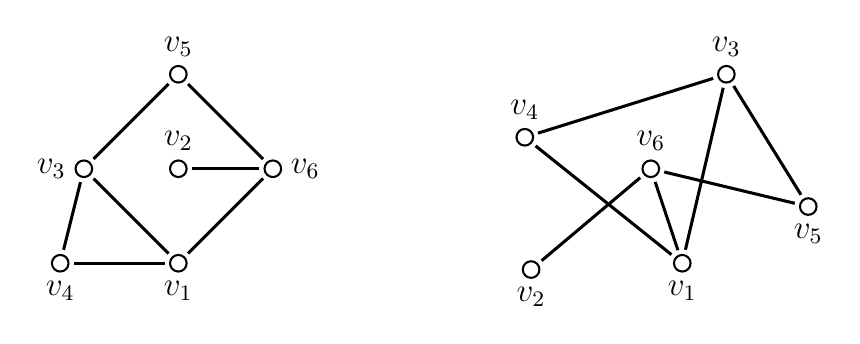
\begin{tikzpicture}
        
            \begin{scope}[xshift=6cm,scale=0.8]
                \draw (0.5,-1.5) node (1) [vertex, label=270:{\large $v_1$}] {};
                \draw (-1.9,-1.6) node (2) [vertex, label=270:{\large $v_2$}] {};
                \draw (1.2,1.5) node (3) [vertex, label=90:{\large $v_3$}] {};
                \draw (-2,0.5) node (4) [vertex, label=90:{\large $v_4$}] {};
                \draw (2.5,-0.6) node (5) [vertex, label=270:{\large $v_5$}] {};
                \draw (0,0) node (6) [vertex, label=90:{\large $v_6$}] {};
                
                \foreach \i/\j in {1/3,1/4,1/6,2/6,3/4,3/5,5/6}
                \draw [edge] (\i) to (\j);
            \end{scope}
    
        \begin{scope}[xshift=0cm,scale=0.6]
            \draw ({(360/4)*3}:2) node(1)[vertex, label=270:{\large $v_1$}]{};
            \draw (0,0) node (2) [vertex, label=90:{\large $v_2$}] {};
            \draw ({(360/4)*2}:2) node(3)[vertex, label=180:{\large $v_3$}]{};
            \draw (-2.5,-2) node (4) [vertex, label=270:{\large $v_4$}] {};
            \draw ({(360/4)*1}:2) node(5)[vertex, label=90:{\large $v_5$}]{};
            \draw ({(360/4)*0}:2) node(6)[vertex, label=0:{\large $v_6$}]{};

            \foreach \i/\j in {1/3,1/4,1/6,2/6,3/4,3/5,5/6}
                \draw [edge] (\i) to (\j);  
            \end{scope}
                
    \end{tikzpicture}
    \caption{Diferentes diagramas de una gr\'afica $G$}
    \label{fig:diagGraf}
\end{figure}

Las gr\'aficas pueden ser representadas por diagramas donde los v\'ertices
son c\'irculos y las arista son l\'ineas cuyos extremos son sus v\'ertices
incidentes. Cabe recalcar que una gr\'afica puede tener m\'ultiples diagramas,
como se muestra en \cref{fig:diagGraf}. Es f\'acil observar que en ambos
diagr\'amas de $G$ los v\'ertices tienen las mismas propiedades, por ejemplo que
$N_G(v_3)=\{v_1,v_4,v_5\}$ o que el grado de $v_2$ es $1$.


Al momento de estudiar objetos matem\'aticos, siempre es importante analizar
como se relacionan dichos objetos entre s\'i. Ya teniendo la noci\'on de una
gr\'afica, ahora nos enfocamos en como se ven las relaciones entre gr\'aficas.
Primero veamos que necesitar\'ian dos gr\'aficas para ser "iguales". Observamos
que, de igual manera que una gr\'afica puede tener varios diagramas, a un
diagr\'ama se le pueden asociar distintas gr\'aficas, renombrando v\'ertices y
aristas para obtener distintos conjuntos de v\'ertices y aristas. Un ejemplo de
esto es \cref{fig:isoGraf}. Al renombrar las aristas de la gr\'afica $G$ como se
muestra en la figura con los colores, podemos dibujar a $G$ como la gr\'afica
$H$ y viseversa. De manera intuitiva, las dos gr\'aficas que comparten un mismo
diagrama podr\'iamos decir que son "iguales" hasta donde nos interesa, pues, al
compartir un diagrama, cumplen muchas propiedades como el n\'umero de
v\'ertices, las adyacencias o el grado de los v\'ertices. Estas g\'aficas se
dice que son isomorfas. Formalmente hablando, dos gr\'aficas $G$ y $H$ son
isomorfas si exite una biyecci\'on $\theta: V(G) \rightarrow V(H)$ tal que para
cualesquiera dos v\'ertices $u, v \in V(G)$, se cumple que $uv \in E(G)$ si y
s\'olo si $\theta(u)\theta(v) \in E(H)$. Es decir, la biyecci\'on $\theta$
preserva adyacencias y no adyacencias. Cuando $G$ es ismorfa a $H$ lo denotamos
$G \cong H$ y la biyecci\'on entre las gr\'aficas es llamada isomorfismo.

\begin{figure}[ht!]
    \centering
       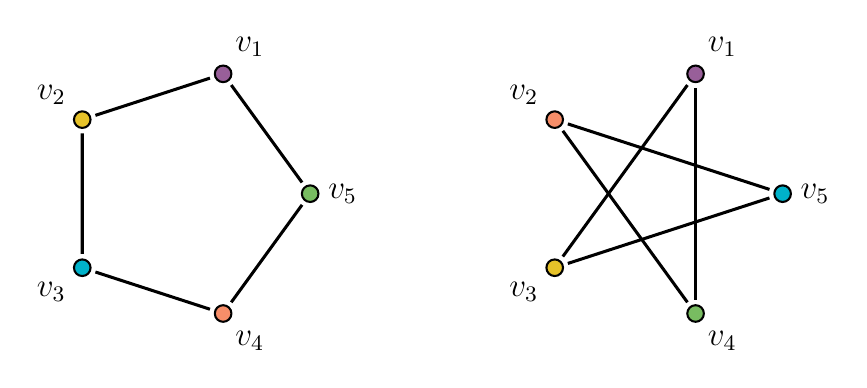
\begin{tikzpicture}
    
            \begin{scope}[xshift=0cm,scale=0.8]
             \draw ({(360/5)*1}:2) node(1)[vertex,fill=morado, label=(360/5)*1:{\large
                    $v_{1}$}]{};
            \draw ({(360/5)*2}:2) node(2)[vertex,fill=amarillo, label=(360/5)*2:{\large
                    $v_{2}$}]{};
           \draw ({(360/5)*3}:2) node(3)[vertex,fill=azulCielo, label=(360/5)*3:{\large
                    $v_{3}$}]{};
            \draw ({(360/5)*4}:2) node(4)[vertex,fill=coral, label=(360/5)*4:{\large
                    $v_{4}$}]{};
            \draw ({(360/5)*5}:2) node(5)[vertex,fill=verde, label=(360/5)*5:{\large
                    $v_{5}$}]{};

            \foreach \i/\j in {5/1,1/2,2/3,3/4,4/5}
                \draw [edge] (\i) to (\j);
            \end{scope}
    
        \begin{scope}[xshift=6cm,scale=0.8]
            \draw ({(360/5)*1}:2) node(1)[vertex,fill=morado, label=(360/5)*1:{\large
            $v_{1}$}]{};
    \draw ({(360/5)*2}:2) node(2)[vertex,fill=coral, label=(360/5)*2:{\large
            $v_{2}$}]{};
   \draw ({(360/5)*3}:2) node(3)[vertex,fill=amarillo, label=(360/5)*3:{\large
            $v_{3}$}]{};
    \draw ({(360/5)*4}:2) node(4)[vertex,fill=verde, label=(360/5)*4:{\large
            $v_{4}$}]{};
    \draw ({(360/5)*5}:2) node(5)[vertex,fill=azulCielo, label=(360/5)*5:{\large
            $v_{5}$}]{};

            \foreach \i/\j in {5/2,2/4,4/1,1/3,3/5}
                \draw [edge] (\i) to (\j);
            \end{scope}
                
    \end{tikzpicture}
    \caption{Dos gr\'aficas isomorfas, la gr\'afica $G$ y la gr\'afica $H$.}
    \label{fig:isoGraf}
\end{figure}

Al momento de ver las relaciones entre dos gr\'aficas, tambi\'en es importante
analizar el caso en el que una gr\'afica sea parte de la otra / "este contenida
en la otra". En el caso de conjuntos nos referir\'iamos a subconjunto y en el
caso de gr\'aficas nos vamos a referir a subgr\'aficas. Sean $G$ y $H$ tales que
$V(H) \subseteq V(G)$ y $E(H) \subseteq E(G)$. Entonces decimos que $H$ es una
subrgr\'afica de $G$. Por otra parte, decimos que $G$ es una supergr\'afica de
$H$. Esta relaci\'on la denotamos con la misma notaci\'on que para subconjuntos,
es decir $H \subseteq G$. Un concepto que se deriva de las subgr\'aficas parte
de fijarnos en la subgr\'afica que tiene la mayor cantidad de aristas posibles.
Formalmente hablando, nos referimos a $H$ la subgr\'afica de $G$ cuyo conjunto
de v\'ertices es $V$ y cuyo conjunto de aristas son aquellas aristas de $G$ que
tienen ambos extremos en $V$, es decir $E(H) = \{uv \in E(G) \colon\ u,v \in
V(H)\}$. A esta subgr\'afica la llamamos la subgr\'afica inducidad de $G$ por
$V$ y la denotamos $G[V]$. Notemos que esta gr\'afica $G[V]$ es la subgr\'afica
de $G$ con conjunto de v\'ertices $V$ que m\'as se parece a $G$. Otro ejemplo
importante de subgr\'aficas es la subgr\'afica inducida obtenida al quitarle
v\'ertices a una gr\'afica. En otras palabras, sea $S \subset V(G)$, nombramos
$H \subseteq G$ a la gr\'afica con $V(H)=V(G) \setminus S$ y $E(H) =
E(G)\setminus\{uv \in E(G) \colon\ u \in S \lor v \in S\}$.Tenemos que $H$ es la
subg\'afica de $G$ obtenida al quitarle el conjunto $S$, esta subgr\'afica la
dentotamos $G-S$. Un caso a se\~{n}alar es cuando $S$ es un conjunto unitario,
es decir, el caso en el que le quitamos un solo v\'ertices $v$ a $G$. En este
caso escribiremos $G-v$ en vez de $G-\{v\}$. A continuaci\'on se muestra un
ejemplo de subgr\'aficas en \cref{fig:subgraf} donde ${\color{morado}H}$ es una
subgr\'afica inducida con $V(G) = \{v_1,v_2,v_3,v_4\}$ y ${\color{azulCielo}H'}$
es una subgr\'afica con $V(H')=\{v_5,v_6,v_7\}$ y $E(H')=\{v_5v_6,  v_6v_7\}$.
Notamos a $H'$ le faltar\'ia la arista ${\color{grisOscuro!80}\bf v_5v_7}$,
resaltada en la figura, para ser una subgr\'afica inducida.


%Como hacer que aparezcan letras con acento usando \color
\begin{figure}[ht!]
    \centering
       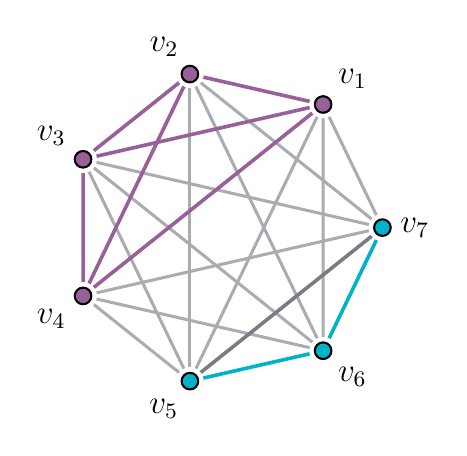
\begin{tikzpicture}
    
            \begin{scope}[xshift=0cm,scale=1]
                \foreach \i in {1,...,4} 
                    \draw ({(360/7)*\i}:2) node(\i)[vertex, fill=morado,
                    label=(360/7)*\i:{\large $v_{\i}$}]{};
                
                \foreach \i in {5,...,7} 
                    \draw ({(360/7)*\i}:2) node(\i)[vertex,fill=azulCielo,
                    label=(360/7)*\i:{\large $v_{\i}$}]{};

            \foreach \i/\j in
                {1/5,1/6,1/7,2/5,2/6,2/7,3/5,3/6,3/7,4/5,
            4/6,4/7}
                \draw [edge,grisOscuro!50] (\i) to (\j);
            
            \foreach \i/\j in
                {1/2,1/3,1/4,2/3,2/4,3/4}
                \draw [wedge,morado] (\i) to (\j);
            
            \foreach \i/\j in
                {5/6,6/7}
                \draw [wedge,azulCielo] (\i) to (\j);
            
            \draw [wedge,grisOscuro!80] (5) to (7);
            \end{scope}
                
    \end{tikzpicture}
    \caption{Una gr\'afica resaltando una ${\color{azulCielo}\bf subgr\'afica}$
    y una ${\color{morado}\bf subgr\'afica inducida}$.}
    \label{fig:subgraf}
\end{figure}


\section{Clanes y conjuntos independientes}
\label{sec:clanes-CIndep}

    Algo que es relevante a trav\'es de varios temas de la Teor\'ia de
     Gr\'aficas es encontrar conjuntos de v\'ertices que sean adyacentes dos a
     dos o conjuntos de v\'ertices que, al contrario, no sean adyacentes a
     ning\'un v\'ertice. Teniendo una gr\'afica $G$ y un conjunto $S \subset
     V(G)$. Decimos que $S$ es independiente si cualesquiera dos v\'ertices de
     $S$ no son adyacentes. Esto quiere decir que todos los elementos de $S$
     tienen grado $0$. La cardinalidad del conjunto independiente m\'as grande
     de una gr\'afica se llama n\'umero de independencia y se denota $\alpha$.
     Por otro lado, decimos que $S$ es un clan si cualesquiera dos v\'ertices en
     $S$ son adyacentes. En este caso, el grado de todo v\'ertice de $S$ es
     $|S-1|$. El n\'umero de clan es la cardinaliad del clan con mayor n\'umero
     de elementos de una gr\'afica, se denota $\omega$. En \cref{fig:ClanInd} se
     muestra un ejemplo de un ${\color{coral}\bf clan}$ y un
     ${\color{verde}\bf conjunto independiente}$ de una gr\'afica. Notemos que
     existe un con clan cardinalidad mayor al ${\color{coral}\bf clan}$ mostrado.
     \'Este clan, llamemoslo $K$, est\'a mostrado con el per\'imetro de los
     v\'ertices de color ${\color{azulCielo}\bf azul}$. Es f\'acil ver que $|K| =
     \omega$.


\begin{figure}[ht!]
    \centering
       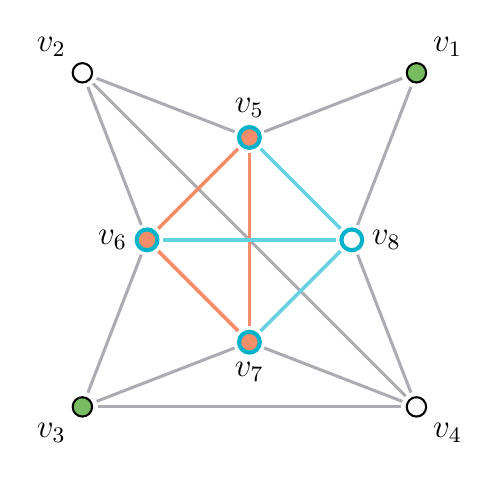
\begin{tikzpicture}
    
            \begin{scope}[xshift=0cm,scale=1]
                \foreach \i in {5,...,7} 
                    \draw ({(360/4)*\i}:1.3) node(\i)[avertex, fill=coral,
                    label=(360/4)*\i:{\large $v_{\i}$}]{};
                \draw ({(360/4)*8}:1.3)node(8)[avertex,label=(360/4)*8:{\large
                    $v_{8}$}]{};
                
                \foreach \i in {1,3} 
                    \draw ({(360/8)*(\i*2-1)}:3) node(\i)[bvertex,fill=verde,
                    label=(360/8)*(\i*2-1):{\large $v_{\i}$}]{};
                
                \foreach \i in {2,4}
                    \draw ({(360/8)*(\i*2-1)}:3)
                   node(\i)[bvertex,label=(360/8)*(\i*2-1):{\large $v_{\i}$}]{};


            \foreach \i/\j in
                {1/5,1/8,2/5,2/6,2/4,3/6,3/7,3/4,4/7,4/8}
                \draw [edge,grisOscuro!50] (\i) to (\j);
            
            \foreach \i/\j in
                {5/6,5/7,6/7}
                \draw [wedge,coral] (\i) to (\j);
            
            \foreach \i/\j in {8/5,8/6,8/7} 
                \draw [wedge,azulCielo!60] (\i) to (\j);
            \end{scope}
                
    \end{tikzpicture}
    \caption{Una gr\'afica, resaltando un dos clanes y un conjunto independiente.}
    \label{fig:ClanInd}
\end{figure}


%notacion de complemento de grafica y el ejemplo de K complemento, que es una
%gr\'afica vacia, es decir su numero de independencia es igual al numero de vertices
\section{Algunas familias relevantes}
\label{sec:famGraf}
\begin{definicion} Tipos de familias de gr\'aficas:
    \label{def:familias}
    \begin{enumerate}
        \item Sea $G$ una gr\'afica, decimos que $G$ es completa si su
        conjunto de aristas es igual a $\binom{V(G)}{2}$.
        \item Una gr\'afica $G$ es una gr\'afica bipartita si su conjunto de
        v\'ertices admite una partici\'on en $X$ y $Y$ de tal manera que $X$ y
        $Y$ son conjuntos independientes. De igual manera, definimos una
        gr\'afica $k$-\textit{partita} como la gr\'afica cuyo conjunto de
        v\'ertices admite una partici\'on en a lo m\'as $k$ conjuntos
        independientes.
        \item Una gr\'afica es bipartita completa si es bipartita y dada la
        partici\'on $X$ y $Y$ de sus v\'ertices, cada v\'ertice de $X$ es
        adyacente a cada v\'ertice de $Y$.   
    \end{enumerate}
\end{definicion}

\section{Tipos de recorridos}
\label{sec:recorridos}


\begin{definicion} Tipos de recorridos de una gr\'afica:
    \label{def:tipos de recorridos}
    \begin{enumerate}
        \item Sea $G$ una gr\'afica, un camino $W$ en $G$ es una sucesi\'on
        alternante de v\'ertices y aristas de $G$ de la siguiente forma $W=(v_0,
        e_1,v_1, \dots, e_{k-1},v_{k-1}, e_k,v_k)$ con $v_i \in V(G)$ y
        $v_{j-1}v_j = e_j \in E(G)$, para $i \in \{0, \dots, k\}$ y $j \in \{ 1,
        \dots, k\}$.
        \item Una trayectoria es un camino que no repite v\'ertices. Llamamos
        $uv$-\textit{trayectoria} a una trayectoria con v\'ertice inicial $u$ y
        \'ultimo v\'ertice $v$.
        \item Decimos que un camino es cerrado si su v\'ertice inicial y su
        v\'ertice final son el mismo.
        \item Un ciclo es un camino cerrado de longitud al menos $3$ que no
        repite v\'ertices, salvo el primer y \'ultimo v\'ertice.
        \item Sea $P$ una trayectoria en una gr\'afica, decimos que $P$ no tiene
        cuerdas si la subgr\'afica inducida por $V(P)$ tiene grado m\'aximo 2.
    \end{enumerate}
\end{definicion}

\section{Conceptos de conexidad}
\label{sec:conexidad}

\begin{definicion} Conceptos de conexidad:
    \label{def:conexidad}
    \begin{enumerate}    
        \item Una gr\'afica $G$ es conexa si para cualquier partici\'on de
        $V(G)$ en dos conjuntos $X$ y $Y$, existe al menos una arista con un
        extremo en $X$ y el otro extremo en $Y$. Si una gr\'afica no es conexa,
        decimos que es inconexa.
        \item Sea $G$ una gr\'afica, nombramos componentes conexas a las
        subr\'aficas de $G$ que son m\'aximas con la propiedad de ser conexas.
        \item Sea $G$ una gr\'afica, un corte por v\'ertices $V$ es un
        subconjunto de $V(G)$ tal que $G[V(G)-V]$ es inconexa.
    \end{enumerate}
\end{definicion}

\section{Conceptos de coloraci\'on}
\label{sec:coloracion}

\begin{definicion} Conceptos de coloraci\'on:
    \label{def:coloracion}
    \begin{enumerate}
        \item Sea $G$ una gr\'afica, una $k$-\textit{coloraci\'on}, o
        simplemente una $\textit{coloraci\'on}$, es una funcion $c \colon
        E(G)\to S$, con $S$ un conjunto de cardinalidad $k$.
        \item Sea $G$ una gr\'afica y $S$ un conjunto de cardinalidad $k$, con
        $k$ entero positivo. La funci\'on $c: V \to S$ es una
        $k$-\textit{coloraci\'on por v\'ertices}, o simplemente una
        $k$-\textit{coloraci\'on}, de $G$. Los elementos de $S$ son llamados
        $\textit{colores}$.
        \item Una coloraci\'on es una \textit{coloraci\'on propia} si todos los
        v\'ertices adyacentes ocupan colores diferentes.
        \item Sea $G$ una gr\'afica y $c$ una coloraci\'on con $S$ colores. Para
        cada color $i \in S$, se define la clase crom\'atica de $i$ de la
        coloraci\'on $c$, denotado $V_i$, como el conjunto de todos los
        v\'ertices de $G$ a que ocupan el color $i$, en otras palabras $V_i =
        c^{-1}[i]$.
        \item  Sea $G$ una gr\'afica, el m\'inimo entero $k$ para el cu\'al $G$
        es $k$-coloreable es el n\'umero crom\'atico de $G$, denotado por
        $\chi(G)$.
    \end{enumerate}
\end{definicion}d

\begin{definicion} Gr\'afica de fichas:
    \label{def:fichas}
    \begin{enumerate}
        \item Sean $G$ una gr\'afica y $k \geq 1$ un entero. Definimos la
        gr\'afica de $k$-fichas de $G$, denotada por $F_k(G)$ como la
        gr\'afica con conjunto de v\'ertices $\binom{V(G)}{k}$ y donde dos
        v\'ertices $A$ y $B$ en $F_k(G)$ son adyacentes si y s\'olo si $|A
        \triangle B| ={a,b}$, con $a \in A$, $b \in B$ y $ab \in E(G)$.
        \item Sea $A$ un $k$-comjunto en la gr\'afica $G$ tal que $a \in A$
        y $b\notin A$. Definimos $A'= (A \setminus \{a\}) \cup \{b\}$.
        \item Sea $P$ una trayectoria en la gr\'afica $G$. Tomamos $A$ un
        $k$- conjunto en $G$ de tal manera que $a\in A$ y $b \notin A$. Si
        $A\cap P =\{v_1, \dots, v_q\}$, con $v_1 = a$, definimos $A
        \xrightarrow[P]{} A'$ como la trayectoria en $F_k(G)$ entre $A$ y
        $A'$ que sigue la siguiente secuencia. Primero movemos la ficha de
        $v_q$, v\'ertice de $G$, hacia el v\'ertice $b$, v\'ertice de $G$,
        por $P$. Luego, para los v\'ertices $v_i$ en $G$,con $i \in \{q-1,
        q-2, \dots 1\}$, movemos la ficha de $v_i$ a $v_{i+1}$. 
    \end{enumerate}
\end{definicion}

\begin{figure}[ht!]
    \centering
       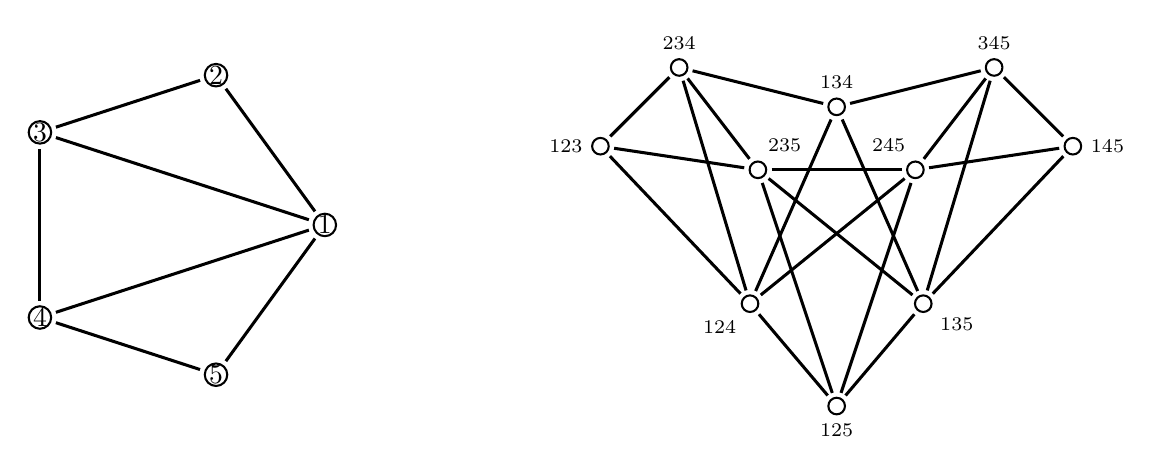
\begin{tikzpicture}
    
        \begin{scope}[xshift=-8.5cm]
            \foreach \i in {0,...,4}
                \draw ({(360/5)*\i}:2) node(\i)[vertex]{\pgfmathparse{int(\i+1)}
                \pgfmathresult};
            \foreach \i/\j in {0/1,0/2,0/3,0/4,1/2,2/3,3/4}
                \draw [edge] (\i) to (\j);
            \end{scope}
        
        \begin{scope}[xshift=0cm,yshift=0cm,scale=1]
            \draw (0,1.5) node (1) [vertex, label=90:{\scriptsize $134$}] {};
            \draw (-2,2) node (2) [vertex, label=90:{\scriptsize $234$}] {};
            \draw (2,2) node (3) [vertex, label=90:{\scriptsize $345$}] {};
            \draw (-3,1) node (4) [vertex, label=180:{\scriptsize $123$}] {};
            \draw (3,1) node (5) [vertex, label=0:{\scriptsize $145$}] {}; 
            \draw (-1,0.7) node (6) [vertex, label=87:{\scriptsize $235$}] {};
            \draw (1,0.7) node (7) [vertex, label=93:{\scriptsize $245$}] {};
            \draw (-1.1,-1) node (8) [vertex, label=240:{\scriptsize $124$}] {};
            \draw (1.1,-1) node (9) [vertex, label=330:{\scriptsize $135$}] {};
            \draw (0,-2.3) node (10) [vertex, label=270:{\scriptsize $125$}] {};
           
            \foreach \i/\j in{1/2, 1/3, 1/8, 1/9, 2/4, 2/6, 2/8, 3/5, 3/7, 3/9,
            4/6, 4/8, 5/7, 5/9, 6/7, 6/9, 6/10, 7/8, 7/10, 8/10, 9/10} 
            \draw [edge] (\i) to (\j);
       \end{scope}
    
            
    
    \end{tikzpicture}
    \caption{El diagrama de una gr\'afica simple $G$ y $F_3(G)$}
    \label{fig:ex-tok-path}
\end{figure}
\chapter{Gr\'aficas de fichas}%
\label{cap:fichass}

\section{Introducci\'on a las gr\'aficas de fichas}%
\label{sec:intro-fichas}


Durante los a\~{n}os 90, se empiezan a estudiar las gr\'aficas de $2$-fichas, en
ese entonces referidas como \textit{Double Vertex Graphs}. Se estudian varias de
sus propiedades, como conectividad, planaridad, regularidad y hamiltonicidad
\cite{alaviPlanarity, alaviDVGraphs, alaviHamilt, zhuConnect}. Al mismo tiempo,
en 1992, se comienzan a estudiar las gr\'aficas de $k$-fichas, para una $k \in
\mathbb{N^{+}}$ m\'as general, refiri\'endose a ellas como \textit{$k$-tuplex
Vertex Graphs} \cite{zhuNTuples}. Posteriormente, en 2002, Rudolph estudia
nuevamente las gr\'aficas de $2$-fichas, presentando un ejemplo de dos
gr\'aficas coespectrales\footnote{La Teor\'ia de Gr\'aficas
Espectrales estudia las gr\'aficas en relaci\'on a su polinomio
caracter\'istico, valores y vectores propios de las matrices asociadas a las
gr\'aficas. Dos gr\'aficas son coespectrales si sus matrices de adyacencia
tienen multiconjuntos de valores propios iguales.}, cuyas gr\'aficas de
$2$-fichas no lo son \cite{rudolphGInv}. En el 2007, se estudian nuevamente las
gr\'aficas de fichas en \cite{audeanetSymPower}, donde se refieren a ellas como
las ``potencias sim\'etricas'' de una gr\'afica. En el art\'iculo, se demuestra
que las gr\'aficas de $2$-fichas de las gr\'aficas fuertemente regulares, con
los mismos par\'ametros, son coespectrales. M\'as adelante, de manera
independiente, Barghi y Ponomarenko \cite{barghi-ponomarenko} y Alzaga, Iglesias
y Pignol \cite{alzagaSymPower} prueban que, para alg\'un entero positivo dado,
existen una cantidad infinita de pares de gr\'aficas no isomorfas con gr\'aficas
de $k$-fichas coespectrales. En el 2012 se reintroduce el concepto de gr\'aficas
de fichas \cite{fabilaToken}, asign\'andole este nombre al pensarlo como
configuraciones de $k$ fichas indistinguibles sobre los v\'ertices de una
gr\'afica $G$, a lo m\'as una ficha por v\'ertice. Una ficha se puede ``mover''
de un v\'ertice de $G$ a otro siempre y cuando exista una arista entre ellos y
no haya una ficha en el segundo v\'ertice. Cada configuraci\'on de $k$ fichas es
un v\'ertice en nuestra nueva gr\'afica, donde dos v\'ertices son adyacentes
siempre que se pueda llegar de una configuraci\'on a otra al mover una ficha a
trav\'es de una arista. A esta nueva gr\'afica la nombramos la gr\'afica de
$k$-fichas de $G$ y la denotamos $F_k(G)$. M\'as adelante, tomando como base
este \'ultimo art\'iculo, se han seguido estudiando propiedades de las
gr\'aficas de fichas como conexidad, planaridad, hamiltonicidad, entre otras
\cite{carballosaRegPlan, leaConnect, riveraHamilt, adameHamilt, leaEConnect}.

Formalmente hablando, dada una gr\'afica $G$ y un entero positivo $k$, la
\textbf{gr\'afica de} $k$-\textbf{fichas} \index{gr\'afica!k @$k$ fichas}
\textbf{de $G$}\index{fichas!gr\'afica} es la gr\'afica cuyo conjunto de
v\'ertices es $\binom{V(G)}{k}$ y donde dos v\'ertices $A$ y $B$ son adyacentes
si y s\'olo si $|A \triangle B| = \{a,b\}$, con $a \in A$, $b \in B$ y $ab \in
E(G)$. Observamos que $F_1(G)$ es isomorfa a $G$, pues cada v\'ertice de
$F_1(G)$ es el v\'ertice de $G$ donde se encuentra la ficha. Por lo mismo, $G$ y
$F_1(G)$ tambi\'en tienen las mismas adyacencias y no adyacencias. Por lo tanto,
en general, nos enfocamos en $F_k(G)$, para $k > 1$. En \cref{fig:ex-tok-graph}
se muestra un ejemplo de una gr\'afica $G$ y su gr\'afica de $2$-fichas. Dentro
de cada v\'ertice de la gr\'afica de $2$-fichas se muestra una copia a escala de
$G$, resaltando en ${\color{rosa}\bf rosa}$ los v\'ertices de $G$ donde se
encuentran las fichas, esto para facilitar el entendimiento de la relacion entre
$G$ y sus gr\'aficas de fichas.

\begin{figure}[ht!]
    \centering
       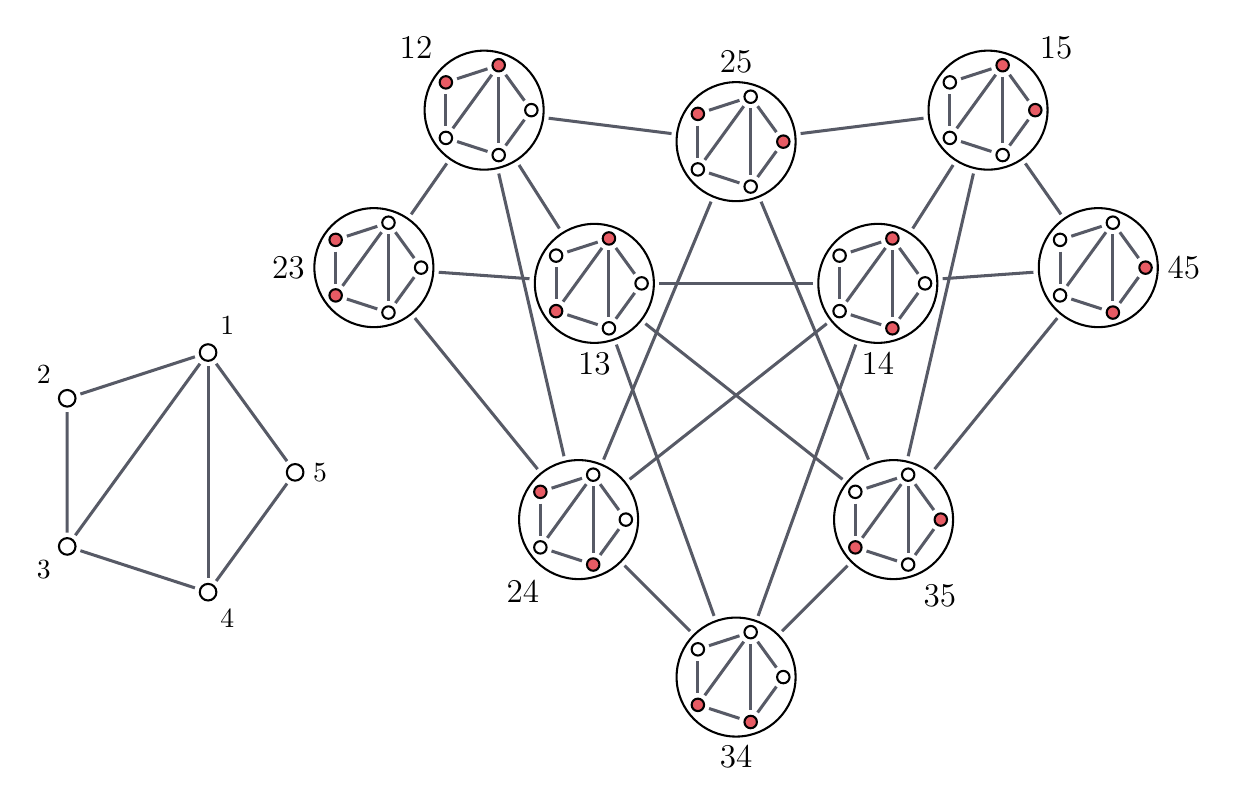
\begin{tikzpicture}
    
        \begin{scope}[xshift=-7.2cm,yshift=-2.6cm,scale=0.8]
            \foreach \i in {1,...,5}
                \draw ({(360/5)*\i}:2) node(\i)[vertex, label=(360/5)*\i:{${\i}$}]{};
            \foreach \i/\j in {1/2,1/3,1/4,1/5,2/3,3/4,4/5}
                \draw [edge,grisOscuro] (\i) to (\j);
        \end{scope}
        
        \begin{scope}[xshift=0cm,yshift=0cm,scale=2]
            \draw (0,-2.6) node (1) [Bvertex, label=270:{\large $34$}] {};
            \draw (0,0.8) node (2) [Bvertex, label=90:{\large $25$}] {};
            \draw (1,-1.6) node (3) [Bvertex, label=290:{\large $35$}] {};
            \draw (-1,-1.6) node (4) [Bvertex, label=240:{\large $24$}] {};
            \draw (2.3,0) node (5) [Bvertex, label=0:{\large $45$}] {}; 
            \draw (-2.3,0) node (6) [Bvertex, label=180:{\large $23$}] {};
            \draw (0.9,-0.1) node (7) [Bvertex, label=270:{\large $14$}] {};
            \draw (-0.9,-0.1) node (8) [Bvertex, label=270:{\large $13$}] {};
            \draw (1.6,1) node (9) [Bvertex, label=45:{\large $15$}] {};
            \draw (-1.6,1) node (10) [Bvertex, label=135:{\large $12$}] {};
           
            \foreach \i/\j in{1/4,1/3,1/7,1/8,2/3,2/4,2/9,2/10,3/5,3/8,3/9,4/6,
            4/7,4/10,5/7,5/9,6/8,6/10,7/8,7/9,8/10} 
            \draw[edge,grisOscuro] (\i) to (\j);
       \end{scope} 
       
       %node (1), $34$
       \begin{scope}[xshift=0cm,yshift=-5.2cm,scale=0.3]
        \foreach \i in {1,2,5}
            \draw ({(360/5)*\i}:2) node(\i)[svertex]{};
        \foreach \i in {3,4}
            \draw ({(360/5)*\i}:2) node(\i)[svertex,fill=rosa]{};
        \foreach \i/\j in {1/2,1/3,1/4,1/5,2/3,3/4,4/5}
            \draw [edge,grisOscuro] (\i) to (\j);
        \end{scope}

        %node (4), $24$
        \begin{scope}[xshift=-2cm,yshift=-3.2cm,scale=0.3]
            \foreach \i in {1,3,5}
                \draw ({(360/5)*\i}:2) node(\i)[svertex]{};
            \foreach \i in {2,4}
                \draw ({(360/5)*\i}:2) node(\i)[svertex,fill=rosa]{};
            \foreach \i/\j in {1/2,1/3,1/4,1/5,2/3,3/4,4/5}
                \draw [edge,grisOscuro] (\i) to (\j);
        \end{scope}

        %node (3), $35$
        \begin{scope}[xshift=2cm,yshift=-3.2cm,scale=0.3]
            \foreach \i in {1,2,4}
                \draw ({(360/5)*\i}:2) node(\i)[svertex]{};
            \foreach \i in {3,5}
               \draw ({(360/5)*\i}:2) node(\i)[svertex,fill=rosa]{};
            \foreach \i/\j in {1/2,1/3,1/4,1/5,2/3,3/4,4/5}
                \draw [edge,grisOscuro] (\i) to (\j);
        \end{scope}

        %node (6), $23$
        \begin{scope}[xshift=-4.6cm,yshift=0cm,scale=0.3]
            \foreach \i in {1,4,5}
                \draw ({(360/5)*\i}:2) node(\i)[svertex]{};
            \foreach \i in {2,3}
                \draw ({(360/5)*\i}:2) node(\i)[svertex,fill=rosa]{};
            \foreach \i/\j in {1/2,1/3,1/4,1/5,2/3,3/4,4/5}
                \draw [edge,grisOscuro] (\i) to (\j);
        \end{scope}
        
        %node (5), $45$
        \begin{scope}[xshift=4.6cm,yshift=0cm,scale=0.3]
            \foreach \i in {1,2,3}
                \draw ({(360/5)*\i}:2) node(\i)[svertex]{};
            \foreach \i in {4,5}
                \draw ({(360/5)*\i}:2) node(\i)[svertex,fill=rosa]{};
            \foreach \i/\j in {1/2,1/3,1/4,1/5,2/3,3/4,4/5}
                \draw [edge,grisOscuro] (\i) to (\j);
        \end{scope}

        %node (8), $13$
        \begin{scope}[xshift=-1.8cm,yshift=-0.2cm,scale=0.3]
            \foreach \i in {2,4,5}
                \draw ({(360/5)*\i}:2) node(\i)[svertex]{};
            \foreach \i in {1,3}
                \draw ({(360/5)*\i}:2) node(\i)[svertex,fill=rosa]{};
            \foreach \i/\j in {1/2,1/3,1/4,1/5,2/3,3/4,4/5}
                \draw [edge,grisOscuro] (\i) to (\j);
        \end{scope}

        %node (7), $14$
        \begin{scope}[xshift=1.8cm,yshift=-0.2cm,scale=0.3]
            \foreach \i in {2,3,5}
                \draw ({(360/5)*\i}:2) node(\i)[svertex]{};
            \foreach \i in {1,4}
                \draw ({(360/5)*\i}:2) node(\i)[svertex,fill=rosa]{};
            \foreach \i/\j in {1/2,1/3,1/4,1/5,2/3,3/4,4/5}
                \draw [edge,grisOscuro] (\i) to (\j);
        \end{scope}

        %node (2), $25$
        \begin{scope}[xshift=0cm,yshift=1.6cm,scale=0.3]
            \foreach \i in {1,3,4}
                \draw ({(360/5)*\i}:2) node(\i)[svertex]{};
            \foreach \i in {2,5}
                \draw ({(360/5)*\i}:2) node(\i)[svertex,fill=rosa]{};
            \foreach \i/\j in {1/2,1/3,1/4,1/5,2/3,3/4,4/5}
                \draw [edge,grisOscuro] (\i) to (\j);
        \end{scope}

        %node (10), $12$
        \begin{scope}[xshift=-3.2cm,yshift=2cm,scale=0.3]
            \foreach \i in {3,4,5}
                \draw ({(360/5)*\i}:2) node(\i)[svertex]{};
            \foreach \i in {1,2}
                \draw ({(360/5)*\i}:2) node(\i)[svertex,fill=rosa]{};
            \foreach \i/\j in {1/2,1/3,1/4,1/5,2/3,3/4,4/5}
                \draw [edge,grisOscuro] (\i) to (\j);
        \end{scope}

        %node (9), $15$
        \begin{scope}[xshift=3.2cm,yshift=2cm,scale=0.3]
            \foreach \i in {2,3,4}
                \draw ({(360/5)*\i}:2) node(\i)[svertex]{};
            \foreach \i in {1,5}
                \draw ({(360/5)*\i}:2) node(\i)[svertex,fill=rosa]{};
            \foreach \i/\j in {1/2,1/3,1/4,1/5,2/3,3/4,4/5}
                \draw [edge,grisOscuro] (\i) to (\j);
        \end{scope}
    
    \end{tikzpicture}
    \caption{Una gr\'afica $G$ (izquierda) y $F_2(G)$ (derecha) donde, dentro de
    cada v\'ertice, se muestra c\'omo es la configuraci\'on de las fichas en $G$
    para dicho v\'ertice.}
    \label{fig:ex-tok-graph}
\end{figure}

Como muchas veces en matem\'aticas, hay ciertas gr\'aficas de fichas que han
sido estudiadas con otro enfoque y bajo otros nombres. Hay un caso que vale la
pena resaltar, el de las gr\'aficas de Johnson. Para un entero $1 \leq k \leq
n$, una \textbf{gr\'afica} \indiceSub{gr\'afica}{de Johnson}, denotada $J(n,k)$,
es la gr\'afica que tiene como conjunto de v\'ertices a todos los
$k$-subconjuntos de $\{1, \dots, n\}$ y donde dos v\'ertices $A$ y $B$ son
adyacentes si y s\'olo si $|A \cap B| = k-1$. Nos fijamos que, para toda $1 \leq
k \leq n$, la gr\'afica de Johnson $J(n,k)$ es isomorfa a la gr\'afica de
$k$-fichas de $K_n$. Las gr\'aficas de Johnson son estudiadas tambi\'en desde la
Teor\'ia de C\'odigos, por lo que hay m\'as ejemplos de este tipo de gr\'aficas
de fichas. De esta manera, las gr\'aficas de Johnson pueden servir como ejemplos
a trav\'es de este trabajo. M\'as a\'un, algunas propiedades conocidas de las
gr\'aficas de Johnson son casos particulares de algunos resultados de este
trabajo.

\section{Algunas estructuras en gr\'aficas de fichas}%
\label{sec:}

Las fichas en una gr\'afica se pueden mover \'unicamente por aristas existentes,
por lo que es natural pensar que una trayectoria en la gr\'afica original tiene
alguna trayectoria en la gr\'afica de fichas con la misma longitud. Teniendo eso
en mente, definimos el siguiente concepto. Sean $P$ una $ab$-trayectoria en la
gr\'afica $G$ y $A$ un $k$-conjunto en $V(G)$, en otras palabras $A \in
V(F_k(G))$. Si al conjunto $A$ le pedimos que $a\in A$ y $b \notin A$, entonces
a la pareja $(A,P)$ le podemos asignar una trayectoria en la gr\'afica de
$k$-fichas, tal que el v\'ertice final est\'a dado por $A'=(A \setminus \{a\})
\cup \{b\}$. Para definir esta nueva trayectoria tomamos $A\cap P =\{v_1, \dots,
v_q\}$, usando el orden en el que los v\'ertices aparecen en $P$ y con $v_1 =
a$. Luego, ``movemos'' las fichas de la siguiente manera. Empezamos, movemos la
ficha de $v_q \in V(G)$ hacia el v\'ertice $b \in V(G)$ por $P$. Despu\'es, para
los v\'ertices $v_i$ en $G$, con $i \in \{q-1, q-2, \dots 1\}$, movemos la ficha
de $v_i$ a $v_{i+1}$ por $P$. As\'i, sucesivamente, vamos moviendo fichas a
trav\'es de $P$ por v\'ertices que est\'an libres de fichas. Observamos que, al
recorrer las fichas a trav\'es de $P$, obtenemos una trayectoria de la misma
longitud que $P$. Esta trayectoria en $F_k(G)$ la denotamos
\indiceSub{fichas}{$A \xrightarrow[P]{} A'$}. A continuaci\'on, se encuentra un
ejemplo de este tipo de trayectoria en una gr\'afica de $3$-fichas, mostrada en
\cref{fig:ex-tok-Path}. Tomamos a \cref{fig:ex-tok-aux} como figura auxiliar
para entender mejor el movimiento de las fichas a trav\'es de la trayectoria. La
gr\'afica $G$ se muestra del lado izquierdo en ambas figuras, adem\'as, en
\cref{fig:ex-tok-Path} se muestra $F_3(G)$ del lado derecho. Definamos
$A=\{2,3,4\}$ en $F_3(G)$ y nuestra trayectoria en $G$ como
${\color{vino}\boldsymbol {P= (3,1,4,5)}}$, resaltada en ambas figuras. De ah\'i
se sigue que $A'=\{2,4,5\}$. Adem\'as, del lado derecho de \cref{fig:ex-tok-aux}
se muestra el movimiento de las fichas que empiezan en $A \cap P =\{3,4\}$,
considerando de arriba a abajo como se van moviendo las fichas.

\begin{figure}[ht!]
    \centering
       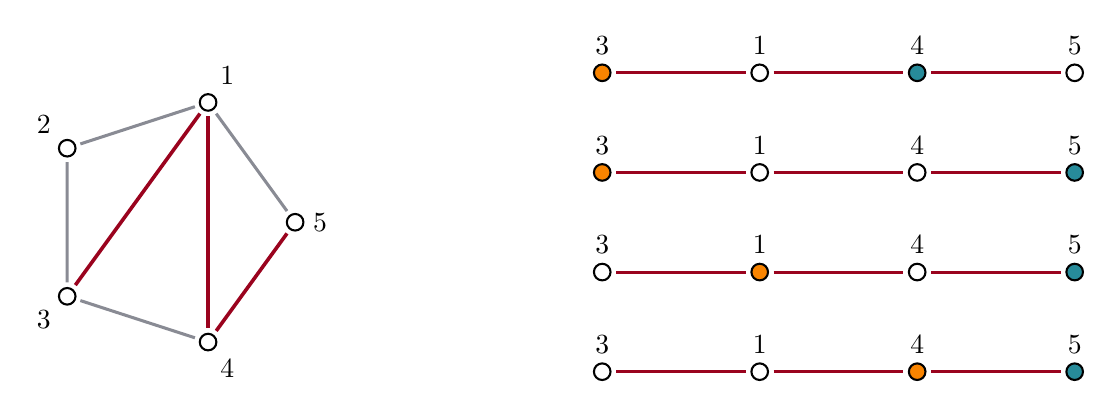
\begin{tikzpicture}
    
        \begin{scope}[xshift=-8.5cm,scale=0.8]
            \foreach \i in {1,...,5}
                \draw ({(360/5)*\i}:2) node(\i)[vertex, label=(360/5)*\i:{${\i}$}]{};
            
            \foreach \i/\j in {1/2,1/5,2/3,3/4}
                \draw [edge,grisOscuro!70] (\i) to (\j);
            \foreach \i/\j in {1/3,1/4,4/5}
                \draw [wedge,vino] (\i) to (\j);
        \end{scope}

        \begin{scope}[yshift=54]
            \draw (-1,0) node (1) [vertex, label=90:{$1$}] {};
            \draw (-3,0) node (3) [vertex, fill=naranja, label=90:{$3$}] {};
            \draw (1,0) node (4) [vertex, fill=azulMetal, label=90:{$4$}] {};
            \draw (3,0) node (5) [vertex, label=90:{$5$}] {};

            \foreach \i/\j in {1/3,1/4,4/5}
                \draw [edge,vino] (\i) to (\j);
        \end{scope}

        \begin{scope}[yshift=18]
            \draw (-1,0) node (1) [vertex, label=90:{$1$}] {};
            \draw (-3,0) node (3) [vertex, fill=naranja, label=90:{$3$}] {};
            \draw (1,0) node (4) [vertex, label=90:{$4$}] {};
            \draw (3,0) node (5) [vertex, fill=azulMetal, label=90:{$5$}] {};

            \foreach \i/\j in {1/3,1/4,4/5}
                \draw [edge,vino] (\i) to (\j);
        \end{scope}

        \begin{scope}[yshift=-18]
            \draw (-1,0) node (1) [vertex, fill=naranja, label=90:{$1$}] {};
            \draw (-3,0) node (3) [vertex, label=90:{$3$}] {};
            \draw (1,0) node (4) [vertex, label=90:{$4$}] {};
            \draw (3,0) node (5) [vertex, fill= azulMetal, label=90:{$5$}] {};

            \foreach \i/\j in {1/3,1/4,4/5}
                \draw [edge,vino] (\i) to (\j);
        \end{scope}

        \begin{scope}[yshift=-54]
            \draw (-1,0) node (1) [vertex, label=90:{$1$}] {};
            \draw (-3,0) node (3) [vertex, label=90:{$3$}] {};
            \draw (1,0) node (4) [vertex, fill=naranja, label=90:{$4$}] {};
            \draw (3,0) node (5) [vertex, fill=azulMetal, label=90:{$5$}] {};

            \foreach \i/\j in {1/3,1/4,4/5}
                \draw [edge,vino] (\i) to (\j);
        \end{scope}
        
    \end{tikzpicture}
    \caption{Una gr\'afica $G$ con una trayectoria $P$ resaltada (izquierda) y
     el movimiento de dos fichas a trav\'es de $P$ (derecho).}
    \label{fig:ex-tok-aux}
\end{figure}
    
M\'as adelante, en \cref{fig:ex-tok-Path}, se muestra la trayectoria
${\color{vino}\boldsymbol {\{2,3,4\}\xrightarrow[P]{}\{2,4,5\}}}$ en $F_3(G)$.
En cada v\'ertice de esta trayectoria se resaltan los n\'umeros del color de la
ficha que se usa en \cref{fig:ex-tok-aux}, para resaltar la relaci\'on entre la
trayectoria de $G$ y la de $F_3(G)$. Observamos que $2$ no est\'a en $A \cap P
=\{3,4\}$, por lo que no se ve en \cref{fig:ex-tok-aux}. Esto significa que la
ficha en el v\'ertice $2$ se queda fija a trav\'es de la trayectoria en la
gr\'afica de fichas. Al estar fija, todos los v\'ertices de la nueva trayectoria
en $F_3(G)$ contienen a $2$. Ese hecho se puede ver en \cref{fig:ex-tok-Path} al
fijarnos que el $2$ est\'a en todos los v\'ertices de la trayectoria, resaltado
en gris.

\begin{figure}[ht!]
    \centering
       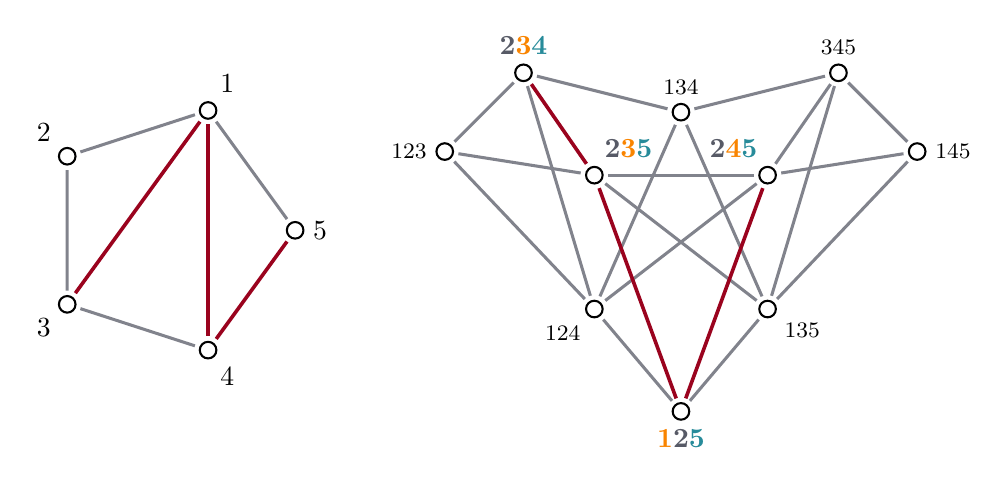
\begin{tikzpicture}
    
        \begin{scope}[xshift=-8.5cm,scale=0.8]
            \foreach \i in {1,...,5}
                \draw ({(360/5)*\i}:2) node(\i)[vertex, label=(360/5)*\i:{\normalsize ${\i}$}]{};
            
            \foreach \i/\j in {1/2,1/5,2/3,3/4}
                \draw [edge,grisOscuro!75] (\i) to (\j);
            \foreach \i/\j in {1/3,1/4,4/5}
                \draw [wedge,vino] (\i) to (\j);
            \end{scope}
        
        \begin{scope}[xshift=-2cm]
            \draw (0,1.5) node (1) [vertex, label=90:{\footnotesize $134$}] {};
            \draw (-2,2) node (2) [vertex, label=90:{${\bf {\color{grisOscuro} 2}{\color{naranja} 3}{\color{azulMetal} 4}}$}] {};
            \draw (2,2) node (3) [vertex, label=90:{\footnotesize $345$}] {};
            \draw (-3,1) node (4) [vertex, label=180:{\footnotesize $123$}] {};
            \draw (3,1) node (5) [vertex, label=0:{\footnotesize $145$}] {}; 
            \draw (-1.1,0.7) node (6) [vertex, label=87:{${\bf {\color{grisOscuro} 2}{\color{naranja} 3}{\color{azulMetal} 5}}$}] {};
            \draw (1.1,0.7) node (7) [vertex, label=93:{${\bf {\color{grisOscuro} 2}{\color{naranja} 4}{\color{azulMetal} 5}}$}] {};
            \draw (-1.1,-1) node (8) [vertex, label=240:{\footnotesize $124$}] {};
            \draw (1.1,-1) node (9) [vertex, label=330:{\footnotesize $135$}] {};
            \draw (0,-2.3) node (10) [vertex, label=270:{${\bf {\color{naranja} 1}{\color{grisOscuro} 2}{\color{azulMetal} 5}}$}] {};
           
            \foreach \i/\j in{1/2,1/3,1/8,1/9,2/4,2/8,3/5,3/7,3/9,4/6,4/8,5/7,
            5/9,6/7,6/9,7/8,8/10,9/10} 
                \draw [edge,grisOscuro!75] (\i)to (\j); 
            \foreach \i/\j in { 2/6,6/10,7/10} 
                \draw [wedge,vino] (\i) to (\j);
       \end{scope}       
    
    \end{tikzpicture}
    \caption{Una gr\'afica $G$, resaltando una trayectoria $P$(derecha) y 
    su gr\'afica de $3$-fichas (izquierda), resaltando la trayectoria 
    generada por $P$.}
    \label{fig:ex-tok-Path}
\end{figure}


Del ejemplo anterior, podemos concluir que tener una ficha fija resulta
interesante al considerar una trayectoria en la gr\'afica de fichas. Vale la
pena analizar c\'omo se comportan otras subgr\'aficas al dejar fija una ficha.
Generalizando un poco m\'as, nos podemos preguntar, qu\'e gr\'afica de
$3$-fichas se obtendr\'ia si una ficha se queda fija, digamos en $2$. Es f\'acil
notar que esta gr\'afica es una subgr\'afica de la gr\'afica de $3$-fichas de
$G$, pues el conjunto de v\'ertices de esta gr\'afica es el conjunto de
v\'ertices de $F_3(G)$ que contengan a $2$. Este ejemplo se representa en
\cref{fig:ex-tok-subgraph}. La idea de fijar una ficha se puede extender a
$r\leq k$ fichas, aunque el caso interesante ser\'a para $r<k$, pues, si fijamos
todas las fichas, obtenemos una gr\'afica trivial. Dado un conjunto $X \subseteq
V(G)$ con $|X|=r<k$, definimos a $F_k(G,X)$ como la \textbf{subgr\'afica de
$F_k(G)$ inducida}\index{subgr\'afica!inducida de
fichas}\index{fichas!subgr\'afica inducida} por los v\'ertices de $F_k(G)$ que
contienen al subconjunto $X$. 

\begin{figure}[ht!]
    \centering
       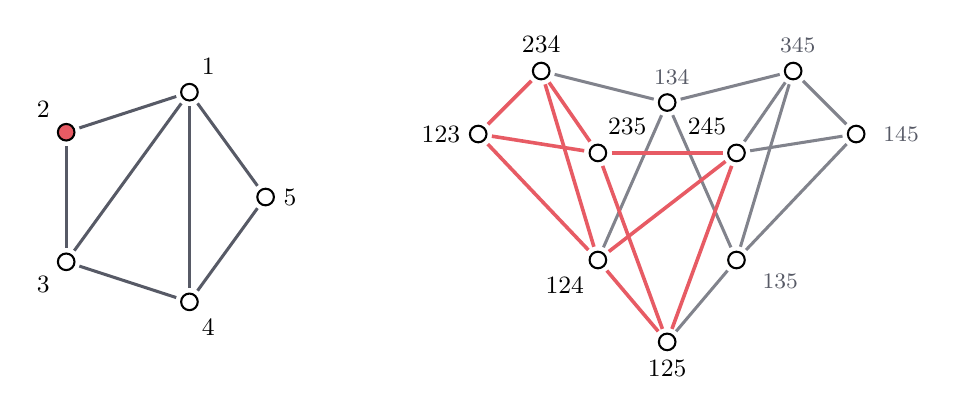
\begin{tikzpicture}
    
        \begin{scope}[xshift=-8.5cm,scale=0.7]
            \foreach \i in {1,3,4,5}
                \draw ({(360/5)*\i}:2) node(\i)[vertex, label=(360/5)*\i:{\small ${\i}$}]{};
            \draw ({(360/5)*2}:2) node(2)[vertex, fill=rosa, label=(360/5)*2:{\small ${2}$}]{};
            
            \foreach \i/\j in {1/2,1/3,1/4,1/5,2/3,3/4,4/5}
                \draw [edge,grisOscuro] (\i) to (\j);
            \end{scope}

        \begin{scope}[xshift=-2cm, scale=0.8]
            \draw (0,1.5) node (1) [vertex, label=90:{{ {\color{grisOscuro}\footnotesize $134$}}}] {};
            \draw (-2,2) node (2) [vertex, label=90:\small $234$] {};
            \draw (2,2) node (3) [vertex, label=90:{{ {\color{grisOscuro}\footnotesize $345$}}}] {};
            \draw (-3,1) node (4) [vertex, label=180:\small $123$] {};
            \draw (3,1) node (5) [vertex, label=0:{{ {\color{grisOscuro}\footnotesize $145$}}}] {}; 
            \draw (-1.1,0.7) node (6) [vertex, label=87:\small $235$] {};
            \draw (1.1,0.7) node (7) [vertex, label=93:\small $245$] {};
            \draw (-1.1,-1) node (8) [vertex, label=240:\small $124$] {};
            \draw (1.1,-1) node (9) [vertex, label=330:{{ {\color{grisOscuro}\footnotesize $135$}}}] {};
            \draw (0,-2.3) node (10) [vertex, label=270:\small $125$] {};
           
            \foreach \i/\j in{1/2,1/3,1/8,1/9,3/5,3/7,3/9,5/7,
            5/9,9/10} 
                \draw [edge,grisOscuro!75] (\i)to (\j); 
            \foreach \i/\j in {2/4,4/6,4/8,2/8,7/8,8/10,2/6,6/7,6/10,7/10} 
                \draw [wedge,rosa] (\i) to (\j);
       \end{scope}       

    \end{tikzpicture}
    \caption{Una gr\'afica $G$ (izquierda) y su gr\'afica de $3$-fichas 
    (derecha), donde se resalta $F_3(G,\{2\})$.}
    \label{fig:ex-tok-subgraph}
\end{figure}

Al momento de generar $F_3(G,{2})$, es f\'acil notar que las fichas se mueven por
$V(G) \setminus \{2\}$, excepto la ficha que est\'a fija. De igual manera, las
aristas por las que se mueven las fichas son las aristas de $G$ que no tienen
extremos en $2$. Vi\'endolo as\'i, podemos interpretar $F_3(G,\{2\})$ como la
gr\'afica de $(3-1)$-fichas de la gr\'afica $G-2$, es decir, $F_2(G-2)$. Esta
gr\'afica est\'a exhibida en \cref{fig:ex-tok-subgraph-aux}. De manera general,
esto quiere decir que existe una relaci\'on entre la subgr\'afica de $F_k(G)$
inducida por $X$, donde $|r|=X \subseteq V(G)$, y la gr\'afica de $(k-r)$-fichas
de la gr\'afica $G-X$, es decir, $F_{k-r}(G-X)$. Afirmamos que, para $k,r \in
\mathbb{N}$ y $k>r = |X|$, con $X \subseteq V(G)$, la gr\'afica $F_k(G,X)$ es
isomorfa a la gr\'afica $F_{k-r}(G-X)$, con el isomorfismo que a cada $A \in
F_k(G,X)$ le asocia $A \setminus X$ en $F_{k-r}(G-X)$.   Observamos que, las
aristas en $G$ con alg\'un extremo en $X$ no se usan en $F_k(G,X)$, por lo que
la funci\'on s\'i preserva adyacencias y no adyacencias.

\begin{figure}[ht!]
    \centering
       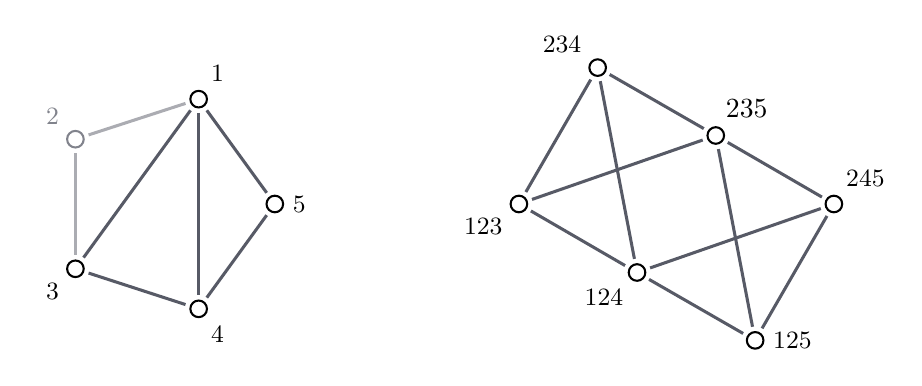
\begin{tikzpicture}
    
       \begin{scope}[xshift=-8.5cm,scale=0.7]
        \foreach \i in {1,3,4,5}
            \draw ({(360/5)*\i}:2) node(\i)[vertex, label=(360/5)*\i:{\small ${\i}$}]{};
        \draw ({(360/5)*2}:2) node(2)[cvertex, label=(360/5)*2:{{ {\color{grisOscuro!75}\small $2$}}}]{};
        
        \foreach \i/\j in {1/3,1/4,1/5,3/4,4/5}
            \draw [edge,grisOscuro] (\i) to (\j);

        \foreach \i/\j in {1/2,2/3}
            \draw [edge,grisOscuro!50] (\i) to (\j);
        \end{scope}

    \begin{scope}[xshift=-2cm]
        \draw (0.5,0.87) node (1) [vertex,label=87:$235$] {};
        \draw ({(360/6)*2}:2) node(2)[vertex, label=(360/5)*2:{\small ${234}$}]{};
        \draw ({(360/6)*3}:2) node(3)[vertex, label=(360/5)*3:{\small ${123}$}]{};
        \draw (-0.5,-0.87) node (4) [vertex,label=240:\small $124$] {};
        \draw ({(360/6)*5}:2) node(5)[vertex, label=(360/5)*5:{\small ${125}$}]{};
        \draw ({(360/6)*6}:2) node(6)[vertex, label=(360/5)*6:{\small ${245}$}]{};
   
    \foreach \i/\j in {1/2,1/3,1/5,1/6,2/3,2/4,3/4,4/5,4/6,5/6}
        \draw [edge,grisOscuro] (\i) to (\j);
    \end{scope}

    \end{tikzpicture}
    \caption{Una gr\'afica $G$ (izquierda), resaltando $G-2$, y la 
    gr\'afica de fichas $F_2(G-2)$ (derecha).}
    \label{fig:ex-tok-subgraph-aux}
\end{figure}

\newpage

Otra cosa interesante del ejemplo de \cref{fig:ex-tok-Path} es que, si nos
fijamos bien, podemos ver que tiene el mismo diagrama que la gr\'afica de
$2$-fichas en \cref{fig:ex-tok-graph}, i.~e., son gr\'aficas isomorfas. Al ser
ambas gr\'aficas de fichas de la misma gr\'afica, vale la pena preguntarse,
cu\'al es la relaci\'on entre ellas. Fij\'andonos a\'un m\'as, vemos que el
isomorfismo entre ambas env\'ia el v\'ertice $A \in V(F_2(G))$ al v\'ertice
$V(G) \setminus A \in V(F_3(G))$. Adem\'as, notamos que dos v\'ertices de $ A,B
\in V(F_2(G))$ son adyacentes si y s\'olo si $V(G) \setminus A$ y $V(G)
\setminus B$ son adyacentes en $F_3(G)$. As\'i, la diferencia sim\'etrica entre
$A$ y $B$ es igual a la diferencia sim\'etrica entre sus complementos. Podemos
verlo como recorrer la gr\'afica ``al rev\'es''. Generalizando este concepto,
afirmamos que, para toda gr\'afica $G$, $F_k(G)$ y $F_{n-k}(G)$ son gr\'aficas
isomorfas. Empezamos viendo que $|V(F_k(G))| =\binom{n}{k}= \binom{n}{n-k}=
|V(F_{n-k}(G))|$. Tomando la funci\'on antes mencionada, falta ver que preserva
adyacencias y no adyacencias. Volviendo a observar que, para todo $A$ y $B$ en
$V(F_k(G))$ tenemos que $A \triangle B = (V(G)\setminus A) \triangle
(V(G)\setminus B)$, entonces las adyacencias y no adyacencias dependen de $G$,
por lo que la funci\'on cumple ser un isomorfismo. 

El resultado anterior resulta de mucha utilidad al momento de estudiar las
gr\'aficas de fichas, pues nos dice que basta en enfocarnos en las gr\'aficas de
$k$-fichas, para $k \leq \frac{n}{2}$.

Teniendo estos isomorfismos en mente, pasamos a desarrollar las propiedades de
las gr\'aficas de fichas mencionadas en los art\'iculos \textit{Token Graphs}
\cite{fabilaToken} y \textit{Hamiltonicity of Token Graphs of Some Join Graphs}
\cite{adameHamilt}.


\section{Di\'ametro y producto cartesiano}%
\label{sec:etiquetas}

En esta secci\'on estudiamos dos teoremas del art\'iculo \textit{Token Graphs}
\cite{fabilaToken}, el primero sobre el di\'ametro de una gr\'afica de fichas y
el segundo sobre el producto cartesiano. Pasamos a establecemos una cota para el
di\'ametro de una gr\'afica de fichas. La demostraci\'on d\cref{teo:diamFG} esta basada
en la demostraci\'on del art\'iculo antes mencionado.

\begin{teorema}%
\label{teo:diamFG}
    Si $G$ una gr\'afica conexa con di\'ametro $d$, entonces, $F_{k}(G)$ es
    conexa con di\'ametro, al menos, $k(d -k+1)$ y, a lo m\'as, $d k$.
\end{teorema}

\begin{proof}
    Sean $A$ y $B$ v\'ertices de $F_{k}(G)$. Primero, nos enfocamos en la cota
    superior. Por definici\'on, tenemos que $|A \triangle B| \leq |A \cup B|$,
    con igualdad cuando $A \cap B = \varnothing$. Observamos que, al ser $A$ y
    $B$ v\'ertices de $F_{k}(G)$, tenemos que $|A|=k$ y $|B|=k$, por lo que $|A
    \cup B| \le 2k$. Luego, tenemos que $|A \triangle B| \leq 2k$, por lo que
    $\frac{1}{2} |A \triangle B| \leq k$.

    Buscamos demostrar que el di\'ametro de $F_{k}(G)$ es, a lo m\'as, $d k$,
    por lo que basta demostrar por inducci\'on que, para cualesquiera dos
    v\'ertices $A$ y $B$ de $F_{k}(G)$, hay una $AB$-trayectoria de, a lo m\'as,
    $\frac{d}{2}|A\triangle B|$. Observamos que esto tambi\'en implica que
    $F_{k}(G)$ es conexa.

    Si $A\triangle B=\varnothing$, entonces $A=B$, por lo que no hay nada que
    probar. Ahora consideramos $A$ y $B$, tales que $A\triangle B \neq
    \varnothing$. Tomamos como hip\'otesis que, para cualesquiera dos v\'ertices
    de $F_{k}(G)$, $C$ y $D$, tales que $|C\triangle D|<|A \triangle B|$, existe
    una $CD$-trayectoria con longitud, a lo m\'as, $\frac{d}{2}|C\triangle D|$.
    Al tomar $A\triangle B \neq \varnothing$, tenemos un v\'ertice de $G$ en
    $A\setminus B$ y un v\'ertice en $B\setminus A$, que denotamos $a$ y $b$,
    respectivamente. Dado que el di\'ametro de $G$ es $d$, tenemos que hay una
    $ab$-trayectoria de longitud a lo m\'as $d$, digamos $P$.

    Definimos $A'=(A\setminus \{a\})\cup \{b\}$ y la trayectoria
    $A\xrightarrow[P]{} A'$ en $F_{k}(G)$. Por un lado, observamos que $b\in
    B\cap A'$ y $b\notin B\cap A$. Por otro lado, tenemos que $a \notin A'$, por
    lo que $a\notin A'\cup B$ y $a\notin A\cap B$. Sin embargo, tanto $a$ como
    $b$ est\'an en $A\cup B$. Por eso, tenemos que $a,b \in A\triangle B$ y $a,b
    \notin A'\triangle B$. Ahora, tomamos $v\in A$ tal que $v \neq a$, se sigue
    que $v \in A\triangle B$ si y s\'olo si $v\in A'\triangle B$. Por lo tanto,
    tenemos que $|A'\triangle B|=|A \triangle B|- 2$. Por hip\'otesis inductiva,
    sabemos que hay una $A'B$-trayectoria en $F_{k}(G)$ de longitud, a lo m\'as,
    $\frac{d}{2}|A'\triangle B|$ que, como se observ\'o anteriormente, coincide
    con $\frac{d}{2}|A\triangle B| - d$.

    Sabemos que $A\xrightarrow[P]{} A'$ tiene la misma longitud que $P$, que es,
    a lo m\'as, $d$. Por ello, tenemos una $AB$-trayectoria de la forma
    $A\rightarrow A'\rightarrow B$ que tiene longitud, a lo m\'as,
    $\frac{d}{2}|A\triangle B|-d +d =\frac{d}{2}|A\triangle B|$. Por lo tanto,
    tenemos que $F_{k}(G)$ es conexa y tiene di\'ametro, a lo m\'as, $d k$.

    Ahora, demostramos la cota inferior. Sabemos que $G$ es una gr\'afica conexa
    con di\'ametro $d$, por lo que existen vertices que est\'an a distancia $d$,
    digamos $x$ y $y$. Ahora, construimos una partici\'on de $V$ usando la
    distancia que tiene cada v\'ertice a $x$. Es decir, para cada $i\in [0,d]$,
    sea $V_{i}$ el conjunto de v\'ertices de $G$ a distancia $i$ de $x$. Por
    tanto, tenemos que $V_{0}=\{x\}$ y $y\in V_{d}$. Denotamos $d_x(v)$ a la
    distancia entre $x$ y el v\'ertice $v$.

    Sea $a$ el m\'inimo \'indice para el cu\'al se tiene $k \leq |V_{0}\cup
    V_{1}\cup \cdots \cup V_{a}|$ y sea $b$ el m\'aximo \'indice para el cu\'al
    se tiene $k\leq |V_{b}\cup V_{b+1}\cup \cdots \cup V_{d}|$. Tomamos $A$ un
    $k$-subconjunto de $V_{0}\cup \cdots \cup V_{a}$  tal que $A\subseteq V_{0}$
    o $V_{0}\cup \cdots \cup V_{a-1}\subseteq A$. Adem\'as, tomamos $B$ un
    $k$-subconjunto de $V_{b}\cup \cdots \cup V_{d}$ tal que $B\subseteq V_{d}$
    o $V_{b+1}\cup \cdots \cup V_{d} \subseteq B$. 

    Consideremos una trayectoria entre $A$ y $B$ en $F_{k}(G)$. Cualquier ficha
    inicialmente en $A$, digamos $v \in (G)$, se mueve a alg\'un v\'ertice en
    $B$, digamos $v'\in (G)$. Notamos que todas las aristas de $G$ est\'an
    dentro de alg\'un $V_{i}$ o, a lo m\'as, entre alg\'un $V_{i}$ y $V_{i+1}$,
    con $i\in[0,d]$. As\'i pues, para la ficha en $v$ se necesitan, al menos,
    $d_x(v')-d_x(v)$ movimientos para llegar a $v'$, ocupando s\'olo las aristas
    entre $V_{i}$ y $V_{i+1}$. Por lo tanto, el di\'ametro de $F_{k}(G)$ es, al
    menos, $\sum_{v\in A}(d_x(v')-d_x(v))= \sum_{w\in B}d_x(w)-\sum_{v\in
    A}d_x(v)$. Observamos que, al ser $G$ conexa, toda $V_{i}$ tiene al menos un
    elemento y, por construcci\'on, $V_{i} \cap V_{i+1}=\varnothing$, para toda
    $i\in [0,d]$. Tomamos el caso en el que $|V_{i}|=1$, para toda $i\in [0,d]$.
    Luego, tenemos que $k\leq |V_{b}\cup\cdots\cup
    V_{d}|=|V_{b}|+|V_{b+1}|+\cdots +|V_d|$ $=\sum_{b}^{d}1 = d -b+1$.
    An\'alogamente, tenemos que $k\leq |V_{0}\cup V_{1}\cup \cdots \cup
    V_{a}|=|V_{0}|+|V_{1}|+\cdots + |V_{a}|$ $=\sum_{0}^{a} 1 = a+1$. En ambos
    casos, la cota m\'inima se alcanza en la igualdad, por lo que tomamos
    $a=k-1$ y $b=d-k+1$. Por lo tanto, tenemos que el di\'ametro de $F_{k}(G)$
    es al menos $\sum_{j=d -k+1}^{d}j - \sum_{i=0}^{k-1}i = k(d-k+1)$.
\end{proof}

Es interesante notar que las cotas obtenidos en \cref{teo:diamFG} son
alcanzables. A continuaci\'on se muestran ejemplos para dichas cotas. La cota
inferior se cumple para toda trayectoria de $d +1$ v\'ertices, con $k \leq d
+1$, es decir, una trayectoria de di\'ametro $d$. Es f\'acil observar que, para
toda $k$, obtenemos una gr\'afica de $k$-fichas de di\'ametro $k(d-k+1)$. Para
ejemplificar estas gr\'aficas, consideremos a la trayectoria $P_6$. Recordamos
que $F_2(P_6) \cong F_4(P_6)$, $F_1(P_6) \cong F_5(P_6)$ y $F_6(P_6) \cong K_1$,
por lo que, en \cref{fig:ex-diamP} se muestran las gr\'aficas de $2$ y
$3$-fichas de la $P_6$. Las gr\'aficas $F_2(P_6)$ y $F_3(P_6)$ tienen di\'ametro
$8$ y $9$, respectivamente, i.~e., tiene di\'ametro $k(d-k+1)$.

\begin{figure}[ht!]
    \centering
    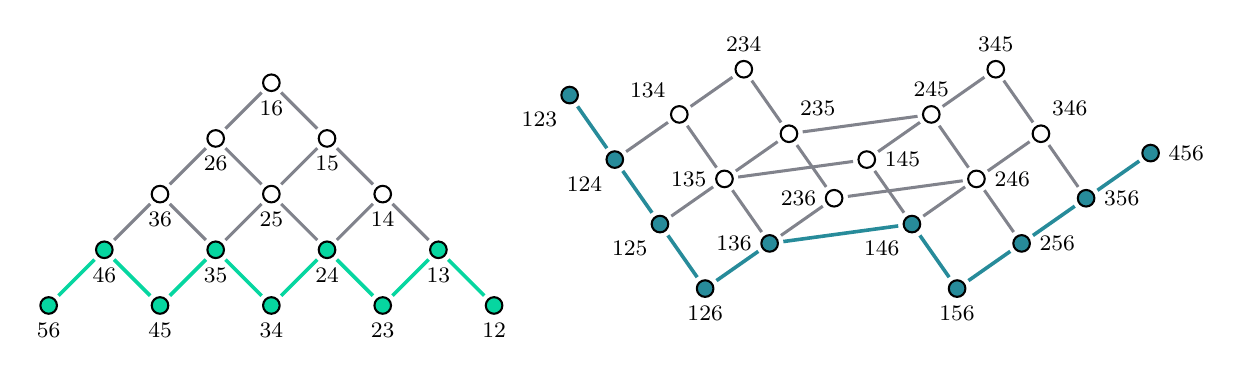
\begin{tikzpicture}
    
        \begin{scope}[xshift=-6cm,yshift=-3cm,rotate=135]
            \draw (2,2) node (1) [vertex,fill=menta,label=270:{\footnotesize $56$}] {};
            \draw (2,1) node (2) [vertex,fill=menta,label=270:{\footnotesize $46$}] {};
            \draw (2,0) node (3) [vertex,label=270:{\footnotesize $36$}] {};
            \draw (2,-1) node (4) [vertex,label=270:{\footnotesize $26$}] {};
            \draw (2,-2) node (5) [vertex,label=270:{\footnotesize $16$}] {};
            \draw (-2,-2) node (6) [vertex,fill=menta,label=270:{\footnotesize $12$}] {};
            \draw (-1,-2) node (7) [vertex,fill=menta,label=270:{\footnotesize $13$}] {};
            \draw (0,-2) node (8) [vertex,label=270:{\footnotesize $14$}] {};
            \draw (1,-2) node (9) [vertex,label=270:{\footnotesize $15$}] {};
            \draw (-1,-1) node (10) [vertex,fill=menta,label=270:{\footnotesize $23$}] {};
            \draw (0,-1) node (11) [vertex,fill=menta,label=270:{\footnotesize $24$}] {};
            \draw (1,-1) node (12) [vertex,label=270:{\footnotesize $25$}] {};
            \draw (0,0) node (13) [vertex,fill=menta,label=270:{\footnotesize $34$}] {};
            \draw (1,0) node (14) [vertex,fill=menta,label=270:{\footnotesize $35$}] {};
            \draw (1,1) node (15) [vertex,fill=menta,label=270:{\footnotesize $45$}] {};

            \foreach \i/\j in{2/3,3/4,4/5,7/8,8/9,5/9,11/12,4/12,
            3/14,9/12,12/14,8/11} 
                \draw [edge,grisOscuro!75] (\i) to (\j);

            \foreach \i/\j in{1/2,2/15,14/15,13/14,11/13,10/11,7/10,6/7} 
                    \draw [wedge,menta] (\i) to (\j);
        \end{scope}
        
        \begin{scope}[rotate=-55]
           
            \draw (2,0) node (21) [vertex,label=180:{\footnotesize $236$}] {};
            \draw (2,-1) node (22) [vertex,fill=azulMetal,label=180:{\footnotesize $136$}] {};
            \draw (2,-2) node (23) [vertex,fill=azulMetal,label=270:{\footnotesize $126$}] {};
            \draw (-1,-2) node (24) [vertex,fill=azulMetal,label=250:{\footnotesize $123$}] {};
            \draw (0,-2) node (25) [vertex,fill=azulMetal,label=250:{\footnotesize $124$}] {};
            \draw (1,-2) node (26) [vertex,fill=azulMetal,label=250:{\footnotesize $125$}] {};
            \draw (0,-1) node (27) [vertex,label=120:{\footnotesize $134$}] {};
            \draw (1,-1) node (28) [vertex,label=180:{\footnotesize $135$}] {};
            \draw (0,0) node (29) [vertex,label=90:{\footnotesize $234$}] {};
            \draw (1,0) node (20) [vertex,label=80:{\footnotesize $235$}] {};
            
            
            \foreach \i/\j in{21/22,27/28,22/28,29/20,
            21/20,29/27,25/27,28/20,26/28} 
                \draw [edge,grisOscuro!75] (\i) to (\j);
        \end{scope}

        \begin{scope}[xshift=3.2cm,yshift=0cm,rotate=-55]
           
            \draw (2,0) node (31) [vertex,fill=azulMetal,label=0:{\footnotesize $356$}] {};
            \draw (2,-1) node (32) [vertex,fill=azulMetal,label=0:{\footnotesize $256$}] {};
            \draw (2,-2) node (33) [vertex,fill=azulMetal,label=270:{\footnotesize $156$}] {};
            \draw (2,1) node (34) [vertex,fill=azulMetal,label=0:{\footnotesize $456$}] {};
            \draw (0,-2) node (35) [vertex,label=0:{\footnotesize $145$}] {};
            \draw (1,-2) node (36) [vertex,fill=azulMetal,label=250:{\footnotesize $146$}] {};
            \draw (0,-1) node (37) [vertex,label=90:{\footnotesize $245$}] {};
            \draw (1,-1) node (38) [vertex,label=0:{\footnotesize $246$}] {};
            \draw (0,0) node (39) [vertex,label=90:{\footnotesize $345$}] {};
            \draw (1,0) node (30) [vertex,label=80:{\footnotesize $346$}] {};
            
            
            \foreach \i/\j in{35/36,37/38,32/38,39/30,
            31/30,39/37,35/37,38/30,36/38} 
                \draw [edge,grisOscuro!75] (\i) to (\j);

           
        \end{scope}
        
        \foreach \i/\j in{24/25,25/26,23/26,22/23,22/36,33/36,32/33,31/32,31/34} 
                    \draw [wedge,azulMetal] (\i) to (\j);
        
                    \foreach \i/\j in{28/35,21/38,20/37} 
            \draw [edge,grisOscuro!75] (\i) to (\j);
        
    \end{tikzpicture}

\caption{La gr\'afica de $2$-fichas (izquierda) y la gr\'afica de $3$-fichas
(derecha) de la trayectoria $P_6$, resaltando una trayectoria de longitud
m\'axima en ambas gr\'aficas.}
\label{fig:ex-diamP}       
\end{figure}

Para la cota superior d\cref{teo:diamFG} consideramos la gr\'afica $G$, obtenida
al a\~{n}adirle $k$ v\'ertices a cada extremo de la trayectoria $P_{d -1}$ y
hacerlos adyacentes a los extremos de esta trayectoria. Observamos que $G$ tiene
di\'ametro $d$. Adem\'as, para toda $k \leq n$, la gr\'afica de $k$-fichas de
$G$ tiene di\'ametro $dk$. Para ejemplificar esto, \cref{fig:ex-diamT} muestra
una gr\'afica $G$ construida al agregar cuatro v\'ertices en cada extremo de la
trayectoria $P_5$, i.~e., $k=4$. Notamos que, la trayectoria que va de
$\{v_1,v_2,v_3,v_4\}$ a $\{w_1,w_2,w_3,w_4\}$ es una trayectoria de longitud
m\'axima. \Cref{fig:ex-diamT} muestra el movimiento de las fichas en $F_4(G)$ de
un extremo al otro. Observamos que, una ficha en alg\'un $v_i$ tiene que moverse
por $d +1$ v\'ertices a alg\'un $w_i$ libre, para $i \in \{1,2,3,4\}$. Adem\'as,
cada movimiento corresponde a un v\'ertice en la trayectoria en $F_4(G)$, que va
de un extremo a otro. Por lo tanto, tenemos que la trayectoria que va de
$\{v_1,v_2,v_3,v_4\}$ a $\{w_1,w_2,w_3,w_4\}$ tiene longitud $4 \cdot 6 = 24$.

\begin{figure}[ht!]
    \centering
       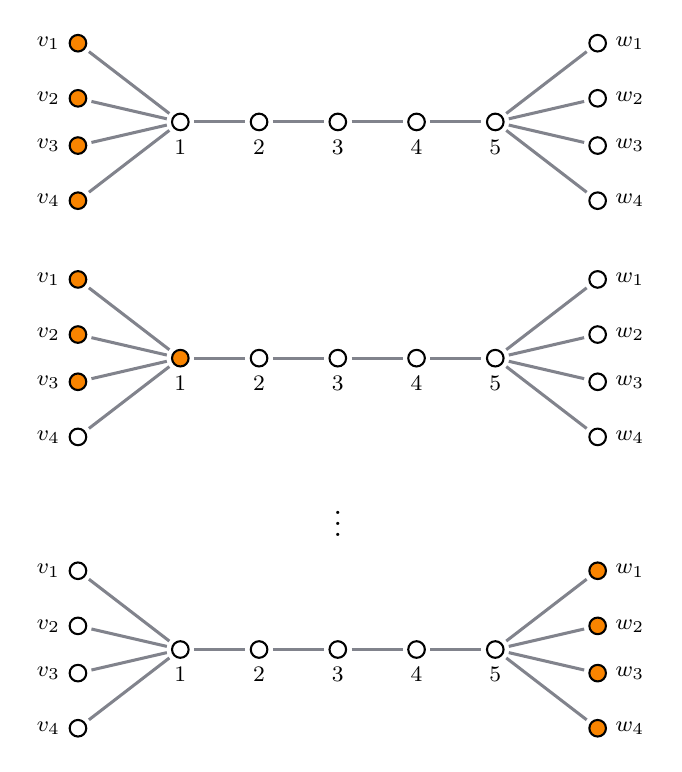
\begin{tikzpicture}
    
        \begin{scope}[]
            \draw (-2,0) node (1) [vertex,label=270:{\footnotesize $1$}] {};
            \draw (-1,0) node (2) [vertex,label=270:{\footnotesize $2$}] {};
            \draw (0,0) node (3) [vertex,label=270:{\footnotesize $3$}] {};
            \draw (1,0) node (4) [vertex,label=270:{\footnotesize $4$}] {};
            \draw (2,0) node (5) [vertex,label=270:{\footnotesize $5$}] {};
            \draw (-3.3,-1) node (6) [vertex,fill=naranja,label=180:{\footnotesize $v_4$}] {};
            \draw (-3.3,-0.3) node (7) [vertex,fill=naranja,label=180:{\footnotesize $v_3$}] {};
            \draw (-3.3,0.3) node (8) [vertex,fill=naranja,label=180:{\footnotesize $v_2$}] {};
            \draw (-3.3,1) node (9) [vertex,fill=naranja,label=180:{\footnotesize $v_1$}] {};
            \draw (3.3,-1) node (10) [vertex,label=0:{\footnotesize $w_4$}] {};
            \draw (3.3,-0.3) node (11) [vertex,label=0:{\footnotesize $w_3$}] {};
            \draw (3.3,0.3) node (12) [vertex,label=0:{\footnotesize $w_2$}] {};
            \draw (3.3,1) node (13) [vertex,label=0:{\footnotesize $w_1$}] {};

            \foreach \i/\j in{1/2,1/6,1/7,1/8,1/9,2/3,3/4,4/5,5/10,5/11,5/12,5/13} 
                \draw [edge,grisOscuro!75] (\i) to (\j);
        \end{scope}

        \begin{scope}[yshift=-3cm]
            \draw (-2,0) node (1) [vertex,fill=naranja,label=270:{\footnotesize $1$}] {};
            \draw (-1,0) node (2) [vertex,label=270:{\footnotesize $2$}] {};
            \draw (0,0) node (3) [vertex,label=270:{\footnotesize $3$}] {};
            \draw (1,0) node (4) [vertex,label=270:{\footnotesize $4$}] {};
            \draw (2,0) node (5) [vertex,label=270:{\footnotesize $5$}] {};
            \draw (-3.3,-1) node (6) [vertex,label=180:{\footnotesize $v_4$}] {};
            \draw (-3.3,-0.3) node (7) [vertex,fill=naranja,label=180:{\footnotesize $v_3$}] {};
            \draw (-3.3,0.3) node (8) [vertex,fill=naranja,label=180:{\footnotesize $v_2$}] {};
            \draw (-3.3,1) node (9) [vertex,fill=naranja,label=180:{\footnotesize $v_1$}] {};
            \draw (3.3,-1) node (10) [vertex,label=0:{\footnotesize $w_4$}] {};
            \draw (3.3,-0.3) node (11) [vertex,label=0:{\footnotesize $w_3$}] {};
            \draw (3.3,0.3) node (12) [vertex,label=0:{\footnotesize $w_2$}] {};
            \draw (3.3,1) node (13) [vertex,label=0:{\footnotesize $w_1$}] {};

            \foreach \i/\j in{1/2,1/6,1/7,1/8,1/9,2/3,3/4,4/5,5/10,5/11,5/12,5/13} 
                \draw [edge,grisOscuro!75] (\i) to (\j);
        \end{scope}


        \begin{scope}[]
            \node at (0,-5) {\large \vdots};
        \end{scope}

        \begin{scope}[yshift=-6.7cm]
            \draw (-2,0) node (1) [vertex,label=270:{\footnotesize $1$}] {};
            \draw (-1,0) node (2) [vertex,label=270:{\footnotesize $2$}] {};
            \draw (0,0) node (3) [vertex,label=270:{\footnotesize $3$}] {};
            \draw (1,0) node (4) [vertex,label=270:{\footnotesize $4$}] {};
            \draw (2,0) node (5) [vertex,label=270:{\footnotesize $5$}] {};
            \draw (-3.3,-1) node (6) [vertex,label=180:{\footnotesize $v_4$}] {};
            \draw (-3.3,-0.3) node (7) [vertex,label=180:{\footnotesize $v_3$}] {};
            \draw (-3.3,0.3) node (8) [vertex,label=180:{\footnotesize $v_2$}] {};
            \draw (-3.3,1) node (9) [vertex,label=180:{\footnotesize $v_1$}] {};
            \draw (3.3,-1) node (10) [vertex,fill=naranja,label=0:{\footnotesize $w_4$}] {};
            \draw (3.3,-0.3) node (11) [vertex,fill=naranja,label=0:{\footnotesize $w_3$}] {};
            \draw (3.3,0.3) node (12) [vertex,fill=naranja,label=0:{\footnotesize $w_2$}] {};
            \draw (3.3,1) node (13) [vertex,fill=naranja,label=0:{\footnotesize $w_1$}] {};

            \foreach \i/\j in{1/2,1/6,1/7,1/8,1/9,2/3,3/4,4/5,5/10,5/11,5/12,5/13} 
                \draw [edge,grisOscuro!75] (\i) to (\j);
        \end{scope}

        
    \end{tikzpicture}
    \caption{La gr\'afica $G$, utilizada como ejemplo d\cref{teo:diamFG},
    resaltando el movimiento de las $4$ fichas al pasar de un extremo de la
    gr\'afica al otro.}
\label{fig:ex-diamT}       
\end{figure}

Nuestro siguiente resultado muestra que algunas subgr\'aficas inducidas de las
gr\'aficas de fichas son productos cartesianos de algunas subgr\'aficas
inducidas de $G$. El art\'iculo \textit{Token graphs} \cite{fabilaToken}, de
donde sale el siguiente teorema, no proporciona una demostraci\'on del dicho
teorema, por lo que la siguiente demostraci\'on es independiente del art\'iculo.

\begin{teorema}
    \label{teo:PCartes}
    Sean $H_1, \dots, H_m$ subgr\'aficas inducidas de una gr\'afica $G$ tales
    que son ajenas dos a dos. Para todos los enteros positivos $s_1, \dots,
    s_m$, tales que $1 \leq s_i \leq |V(H_i)|$ y $\sum\limits_{i=1}^{m}  s_i =
    k$, se tiene que $F_{s_1}(H_1) \square \cdots \square F_{s_m}(H_m)$ es una
    subgr\'afica inducida de $F_k(G)$.
\end{teorema}

\begin{proof}
    Sean $H_1, \dots, H_m$ subgr\'aficas inducidas de  $G$ y sean $s_1, \dots,
    s_m \in \mathbb{Z}$ como en el enunciado. Al conjunto de los
    $k$-subconjuntos de $G$ que cumplen tener exactamente $s_i$ elementos de
    $H_i$, para $i \in \{1, \dots, m\}$, lo llamamos $L$, i.~e., $L = \{A
    \subseteq G \colon\ |A\cap V(H_1)|=s_1 , |A \cap V(H_2)|=s_2, \dots, |A \cap
    V(H_m)|=m \}$. Observamos que, debido a  que $\sum\limits_{i=1}^{m} s_i =
    k$, todo elemento de $L$ tiene cardinalidad $k$. Buscamos ver que la
    subgr\'afica inducida de $F_k(G)$ por $L$, es decir, $F_k(G,L)$, es isomorfa
    a $F_{s_1}(H_1) \square \cdots \square F_{s_m}(H_m)$. Primero, analizamos el
    conjunto de v\'ertices de ambas gr\'aficas de fichas. Sea $A \in
    V(F_k(G,L))$, de tal manera que $A=\{a_1, \dots, a_{s_1}, b_1,\dots,
    b_{s_2}, \dots, m_1, \dots, m_{s_m}\}$. Por definici\'on, $|A \cap V(H_i)|=
    s_i$, para $i \in \{1, \dots, m\}$. Adem\'as, sabemos que cada v\'ertice de
    $F_{s_i}(H_i)$ tiene cardinalidad $s_i$, para $i \in \{1, \dots, m\}$, por
    lo que tenemos que $A \in V(H_1) \times \cdots \times V(H_m)$. De manera
    an\'aloga, si tomamos $A \in V(H_1) \times \cdots \times V(H_m)$, $A =
    \{A'_1, A'_2, \dots, A'_m\}$ con $A'_i \in F_{s_i}(H_i)$. De lo anterior,
    tenemos que $A \cap V(H_i) = A'_i$, por lo que $|A \cap V(H_i)|= s_i$, para
    toda $i \in \{1, \dots, m\}$. Adicionalmente, tenemos que $|A|= k$, puesto
    que $\sum\limits_{i=1}^{m} s_i = k$. Por lo tanto, $A \in V(F_k(G,L))$.

    Ahora, nos enfocamos en la relaci\'on entre las aristas de ambas gr\'aficas
    de fichas. Sean $B, C \in V(F_k(G,L))$, tales que $BC \in E(F_k(G,L))$, en
    otras palabras, existen $b \in B$ y $c \in C$, tales que $B \triangle C =
    \{b, c\}$ y $bc \in E(G[L])$. Por definici\'on, tenemos que $V(H_i) \cap
    V(H_j) = \varnothing$, con $i \neq j$, por lo que $b, c \in V(H_i)$. Esto
    significa que las fichas en $H_j$ est\'an est\'aticas, para todo $j \in \{1,
    \dots, m\} \setminus \{i\}$. Lo cu\'al pasa si y s\'olo s\'i $BC$ es una
    arista en la subgr\'afica de fichas inducida por $H_i$. Como $V(H_i) \cap
    V(H_j) = \varnothing$, para $i \neq j$, entonces la subgr\'afica de fichas
    inducida por $H_i$ es isomorfa a $F_{s_i}(H_i)$. Al tener el resto de las
    fichas est\'aticas, tenemos que $BC \in E(F_{s_1}(H_1) \square \cdots
    \square F_{s_m}(H_m))$.

    Por tanto, tenemos un isomorfismo entre $F_{s_1}(H_1) \square \cdots
    \square F_{s_m}(H_m)$ y $F_k(G,L)$, una subgr\'afica inducida de $F_k(G)$.
    Por ende, $F_{s_1}(H_1) \square \cdots \square F_{s_m}(H_m)$ es una
    subgr\'afica inducida de $F_k(G)$.
\end{proof}

\Cref{fig:ex-cart}, exhibida a continuaci\'on, es un ejemplo sencillo
d\cref{teo:PCartes}. Del lado izquierdo de la figura tenemos una gr\'afica $G$,
resaltando dos subgr\'aficas inducidas ${\color{baige}\boldsymbol {H_1}}$ y
${\color{azulMetal}\boldsymbol {H_2}}$. El conjunto de v\'ertices de
${\color{azulMetal}\boldsymbol {H_2}}$ es $\{1,2,4,6\}$, mientras que el de
${\color{baige}\boldsymbol {H_1}}$ es $\{3\}$. Por un lado tenemos que $1\leq
s_1 \leq |V(H_1)|$, por lo que $s_1 =1$. Por otro lado, $1\leq s_2 \leq |V(H_2)|
= 4$ y, adem\'as, $s_1+s_2 = k =3$, por lo que $s_2 =2$. Del lado derecho de
\cref{fig:ex-cart} se muestra la gr\'afica $F_3(G)$, resaltando de
$\color{fushia} \bf rosa$ el producto cartesiano $F_1(H_1) \square F_2(H_2)$.
Observamos que dicha gr\'afica es, en efecto, una subgr\'afica inducida de
$F_3(G)$.

\begin{figure}[ht!]
    \centering
       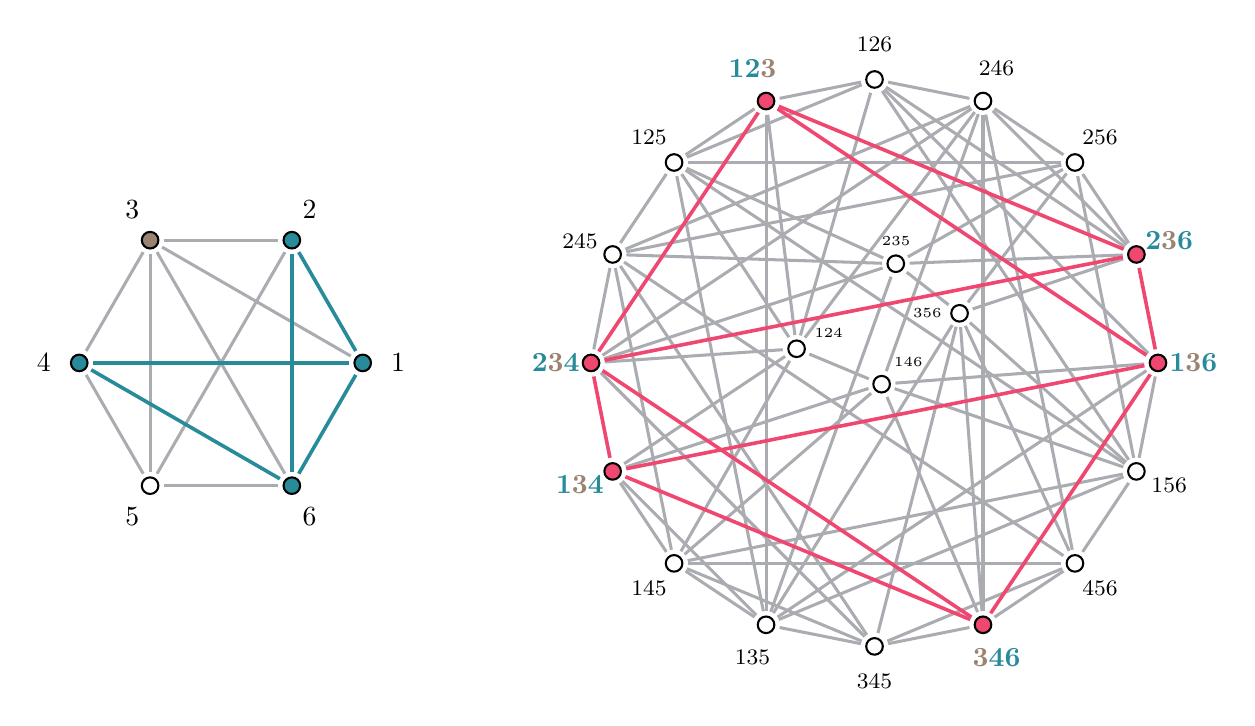
\begin{tikzpicture}
    
        \begin{scope}[xshift=-8.5cm,scale=0.9]
            \foreach \i in {0,1,3,5}
                \draw ({(360/6)*\i}:2) node(\i)[wvertex,fill=azulMetal]{};
            \draw ({(360/6)*2}:2) node(2)[wvertex,fill=baige]{};
            \draw ({(360/6)*4}:2) node(4)[wvertex]{}; 
            \foreach \i in {0,...,5}
                \draw ({(360/6)*\i}:2.5) node(e0){\pgfmathparse{int(\i+1)}
               \pgfmathresult};
            \foreach \i/\j in {0/2,1/2,1/4,2/3,2/4,2/5,3/4,4/5}
                \draw [edge,grisOscuro!50] (\i) to (\j);
            
            \foreach \i/\j in {0/1,0/5,0/3,1/5,3/5}
                \draw [wedge,azulMetal] (\i) to (\j); 
            \end{scope}
        
        \begin{scope}[xshift=-0.2cm,yshift=0cm,scale=0.9]
            \foreach \i in {0,1,5,8,9,13} 
                \draw ({(360/16)*\i}:4) node(\i)[wvertex,fill=fushia]{}; 
            \foreach \i in {2,3,4,6,7,10,11,12,14,15} 
                \draw({(360/16)*\i}:4) node(\i)[wvertex]{};
    
            \draw ({(360/16)*1}:4.5) node (e1) {{${\color{azulMetal}\bf 2}{\color{baige}\bf 3}{\color{azulMetal}\bf6}$}};
            \draw ({(360/16)*2}:4.5) node (e1) {{\footnotesize $256$}};
            \draw ({(360/16)*3}:4.5) node (e1) {{\footnotesize $246$}};
            \draw ({(360/16)*4}:4.5) node (e1) {{\footnotesize $126$}};
            \draw ({(360/16)*5}:4.5) node (e1) {{${\color{azulMetal}\bf12}{\color{baige}\bf 3}$}};
            \draw ({(360/16)*6}:4.5) node (e1) {{\footnotesize $125$}};
            \draw ({(360/16)*7}:4.5) node (e1) {{\footnotesize $245$}};
            \draw ({(360/16)*8}:4.5) node (e1) {{${\color{azulMetal}\bf2}{\color{baige}\bf 3}{\color{azulMetal}\bf4}$}};
            \draw ({(360/16)*9}:4.5) node (e1) {{${\color{azulMetal}\bf1}{\color{baige}\bf 3}{\color{azulMetal}\bf4}$}};
            \draw ({(360/16)*10}:4.5) node (e1) {{\footnotesize $145$}};
            \draw ({(360/16)*11}:4.5) node (e1) {{\footnotesize $135$}};
            \draw ({(360/16)*12}:4.5) node (e1) {{\footnotesize $345$}};
            \draw ({(360/16)*13}:4.5) node (e1) {{${\color{baige}\bf 3}{\color{azulMetal}\bf46}$}};
            \draw ({(360/16)*14}:4.5) node (e1) {{\footnotesize $456$}};
            \draw ({(360/16)*15}:4.5) node (e1) {{\footnotesize $156$}};
            \draw ({(360/16)*16}:4.5) node (e1) {{${\color{azulMetal}\bf1}{\color{baige}\bf 3}{\color{azulMetal}\bf6}$}};
    
            \draw (-1.1,0.2) node (17) [vertex,label=10:{\tiny $124$}] {};
            \draw (0.1,-0.3) node (18) [vertex,label=70:{\tiny $146$}] {};
            \draw (1.2,0.7) node (19) [vertex,label=180:{\tiny $356$}] {};
            \draw (0.3,1.4) node (20) [vertex,label=88:{\tiny $235$}] {};
            
            \foreach\i/\j in{0/4,0/11,0/15,0/18,1/2,1/3,1/4,1/19,1/20,2/3,2/6,
            2/7,2/15,2/19,2/20,3/4,3/7,3/8,3/13,3/14,3/17,3/18,4/5,4/6,4/15,4/17,
            5/6,5/11,5/17,6/7,6/11,6/15,6/17,6/20,7/8,7/10,7/12,7/14,7/20,8/12,
            8/17,8/20,9/10,9/11,9/17,9/18,10/11,10/12,10/14,10/15,10/17,10/18,
            11/12,11/15,11/19,11/20,12/13,12/14,12/19,13/14,13/18,13/19,14/15,
            14/19,15/18,15/19,17/18,19/20} 
               \draw [edge,grisOscuro!50] (\i) to (\j);

               \foreach \i/\j in {0/1,0/5,0/9,0/13,1/5,1/8,5/8,8/9,8/13,9/13}
               \draw [wedge,fushia] (\i) to (\j);
       \end{scope}

    \end{tikzpicture}
    \caption{Una gr\'afica $G$ (izquierda), resaltando dos subgr\'aficas
    inducidas, ${\color{baige}\boldsymbol {H_1}}$ y
    ${\color{azulMetal}\boldsymbol {H_2}}$. $F_3(G)$ (derecha), resaltando su
    subgr\'afica inducida ${\color{fushia}\boldsymbol {F_1(H_1) \square
    F_2(H_2)}}$.}
    \label{fig:ex-cart}
    \end{figure}
\chapter{Conexidad}%
\label{cap:conexidad}

En este cap\'itulo nos enfocaremos en la conexidad de las gr\'aficas de fichas.
Estableceremos algunas cotas para el di\'ametro y el n\'umero de trayectorias
internamente ajenas que se pueden encontrar en una gr\'afica de fichas,
bas\'andonos en las caractere\'isticas y par\'ametros de las gr\'aficas de las
cu\'ales provienen.

\section{Algunas propiedades interesantes}%
\label{sec:etiquetas}

En esta secci\'on veremos algunas peque\~{n}as propiedades que pueden
resultar interesantes. Primero estableceremos una cota para el di\'ametro de una
gr\'afica de fichas.

\begin{teorema}%
\label{teo:diamFG}
Sea $G$ una gr\'afica conexa con di\'ametro $d$. Entonces, $F_{k}(G)$ es 
conexa con di\'ametro al menos $k(d -k+1)$ y a lo m\'as $d k$.
\end{teorema}

\begin{proof}
Sean $A$ y $B$ v\'ertices de $F_{k}(G)$. Primero nos enfocamos en la cota
superior. Por definici\'on tenemos que $|A \triangle B| \leq |A \cup B|$, con
igualdad cuando $A \cap B = \varnothing$. Observamos que, al ser $A$ y $B$
v\'ertices de $F_{k}(G)$, tenemos que $|A|=k$ y $|B|=k$ por lo que $|A \cup B|
\le 2k$. Entonces, tenemos que $|A \triangle B| \leq 2k$, por lo que
$\frac{1}{2} |A \triangle B| \leq k$.

Buscamos demostrar que el di\'ametro de $F_{k}(G)$ es a lo m\'as $d k$, por
lo que basta demostrar, por inducci\'on, que para cualesquiera dos v\'ertices
$A$ y $B$ de $F_{k}(G)$ hay una $AB$-trayectoria de a lo m\'as
$\frac{d}{2}|A\triangle B|$. Observamos que esto tambi\'en implica que
$F_{k}(G)$ es conexa.

Si $A\triangle B=\varnothing$, entonces $A=B$, por lo que no hay nada que probar.
Ahora consideramos $A$ y $B$ tales que $A\triangle B \neq \varnothing$. Tomamos
como hip\'otesis que para cualesquiera dos v\'ertices de $F_{k}(G)$, $C$ y $D$,
tales que $|C\triangle D|<|A \triangle B|$, existe una $CD$-trayectoria con
longitud a lo m\'as $\frac{d}{2}|C\triangle D|$. Al tomar $A\triangle B
\neq \varnothing$ tenemos un v\'ertice de $G$ en $A\setminus B$ y un v\'ertice
en $B\setminus A$, que denotamos $a$ y $b$, respectivamente. Dado que el
di\'ametro de $G$ es $d$, entonces hay una $ab$-trayectoria de longitud a
lo m\'as $d$, digamos $P$.

Definimos $A'=(A\setminus \{a\})\cup \{b\}$ y la trayectoria $A\xrightarrow[P]{}
A'$ en $F_{k}(G)$. Observamos que, por un lado $b\in B\cap A'$ y $b\notin B\cap
A$, pero $b\in A\cup B$. Por otro lado tenemos que $a\notin A'$ por lo que
$a\notin A'\cup B$ y $a\notin A\cap B$, pero $a\in A\cup B$. Entonces, tenemos
que $a,b \in A\triangle B$ y $a,b \notin A'\triangle B$. Ahora tomamos $v\in A$
tal que $v \neq a$. Entonces, tenemos que $v \in A\triangle B$ si y s\'olo si
$v\in A'\triangle B$. Por lo tanto tenemos que $|A'\triangle B|=|A \triangle B|-
2$. Por hip\'otesis inductiva, sabemos que hay una $A'B$-trayectoria en
$F_{k}(G)$ de longitud a lo m\'as $\frac{d}{2}|A'\triangle B|$, que como se
observ\'o anteriormente, coincide con $\frac{d}{2}|A\triangle B| - d$.

Sabemos que $A\xrightarrow[P]{} A'$ tiene la misma longitud que $P$, que es a lo
m\'as $d$. Entonces, tenemos una $AB$-trayectoria de la forma $A\rightarrow
A'\rightarrow B$ que tiene longitud a lo m\'as $\frac{d}{2}|A\triangle
B|-d +d =\frac{d}{2}|A\triangle B|$. Por lo tanto tenemos que
$F_{k}(G)$ es conexa y tiene di\'ametro a lo m\'as $d k$.

Ahora demostraremos la cota inferior. Sabemos que $G$ es una gr\'afica conexa
con di\'ametro $d$, por lo que existen vertices que est\'an a distancia
$d$, digamos $x$ y $y$. Ahora construimos una partici\'on de $V$ usando  la
distancia que tiene cada v\'ertice a $x$. Es decir, para cada $i\in [0,d]$,
sea $V_{i}$ el conjunto de v\'ertices de $G$ a distancia $i$ de $x$. Entonces,
tenemos que $V_{0}=\{x\}$ y $y\in V_{d}$. Denotamos $d_x(v)$ a la distancia
entre $x$ y el v\'ertice $v$.

Sea $a$ el m\'\i{}nimo \'\i{}ndice para el cu\'al se tiene $k \leq |V_{0}\cup
V_{1}\cup \cdots \cup V_{a}|$ y sea $b$ el m\'aximo \'\i{}ndice para el cu\'al se
tiene $k\leq |V_{b}\cup V_{b+1}\cup \cdots \cup V_{d}|$. Tomamos $A$ un
$k$-subconjunto de $V_{0}\cup \cdots \cup V_{a}$  tal que $A\subseteq
V_{0}$ o $V_{0}\cup \cdots \cup V_{a-1}\subseteq A$. Tomamos $B$ un
$k$-subconjunto de $V_{b}\cup \cdots \cup V_{d}$ tale que
$B\subseteq V_{d}$ o $V_{b+1}\cup \cdots \cup V_{d}$. 

Consideramos cualquier trayectoria entre $A$ y $B$ en $F_{k}(G)$. Cualquier
ficha inicialmente en $A$, digamos en el v\'ertice $v$ de $G$, se mueve a
alg\'un v\'ertice en $B$, digamos el v\'ertice $v'$ de $G$. Observamos que todas
las aristas de $G$ est\'an dentro de alg\'un $V_{i}$ o a lo m\'as entre alg\'un
$V_{i}$ y $V_{i+1}$, con $i\in[0,d]$. Entonces, para la ficha en $v$ se
necesitan al menos $d_x(v')-d_x(v)$ movimientos para llegar a $v'$, ocupando
s\'olo las aristas entre $V_{i}$ y $V_{i+1}$, $i\in [0,d]$. Por lo tanto,
el di\'ametro de $F_{k}(G)$ es al menos $\sum_{v\in A}(d_x(v')-d_x(v))=
\sum_{w\in B}d_x(w)-\sum_{v\in A}d_x(v)$. Observamos que, al ser $G$ conexa,
toda $V_{i}$ tiene al menos un elemento y por construcci\'on $V_{i} \cap
V_{i+1}=\varnothing$, para toda $i\in [0,d]$. Tomamos el caso en el que
$|V_{i}|=1$ para toda $i\in [0,d]$. Entonces, tenemos que $k\leq
|V_{b}\cup\cdots\cup V_{d}|=|V_{b}|+|V_{b+1}|+\cdots +|V_d|$
$=\sum_{b}^{d}1 = d -b+1$. An\'alogamente tenemos que $k\leq
|V_{0}\cup V_{1}\cup \cdots \cup V_{a}|=|V_{0}|+|V_{1}|+\cdots + |V_{a}|$
$=\sum_{0}^{a} 1 = a+1$ En ambos casos la cota m\'\i{}nima se alcanza en la
igualdad, por lo que tomamos $a=k-1$ y $b=d-k+1$. Por lo tanto tenemos que
el di\'ametro de $F_{k}(G)$ es al menos $\sum_{j=d -k+1}^{d}j -
\sum_{i=0}^{k-1}i = k(d-k+1)$.
\end{proof}

Es interesante notar que las cotas obtenidos en \cref{teo:diamFG} son
alcanzables. A continuaci\'on se muestran algunos ejemplos para dichas cotas. La
cota inferior se cumple para toda trayectoria de $d +1$ v\'ertices, con $k \leq
d +1$, es decir una trayectoria de di\'ametro $d$. Es f\'acil observar que para
toda $k$ obtenemos una gr\'afica de $k$-fichas de di\'ametro $k(d-k+1)$. Para
ejemplificar este tipo de gr\'aficas consideremos la trayectoria $P_6$.
Recordamos que $F_2(P_6) \cong F_4(P_6)$, $F_1(P_6) \cong F_5(P_6)$ y $F_6(P_6)
\cong K_1$.La Figura\ref{fig:ex-diamP} muestra las gr\'aficas de $2$ y
$3$-fichas de la $P_6$. Las gr\'aficas $F_2(P_6)$ y $F_3(P_6)$ tienen di\'ametro
$8$ y $9$, respectivamente, i.e. tiene di\'ametro $k(d-k+1)$

\begin{figure}[ht!]
    \centering
    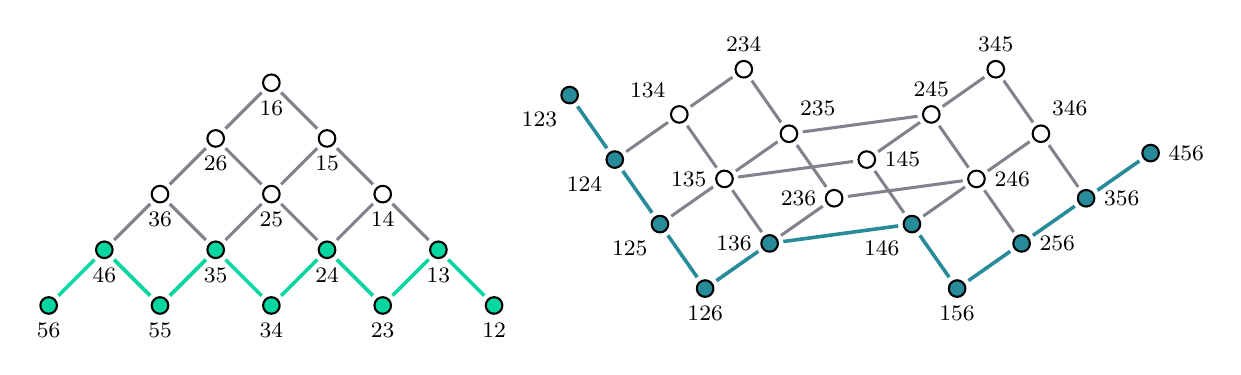
\begin{tikzpicture}
    
        \begin{scope}[xshift=-6cm,yshift=-3cm,rotate=135]
            \draw (2,2) node (1) [vertex,fill=menta,label=270:{\footnotesize $56$}] {};
            \draw (2,1) node (2) [vertex,fill=menta,label=270:{\footnotesize $46$}] {};
            \draw (2,0) node (3) [vertex,label=270:{\footnotesize $36$}] {};
            \draw (2,-1) node (4) [vertex,label=270:{\footnotesize $26$}] {};
            \draw (2,-2) node (5) [vertex,label=270:{\footnotesize $16$}] {};
            \draw (-2,-2) node (6) [vertex,fill=menta,label=270:{\footnotesize $12$}] {};
            \draw (-1,-2) node (7) [vertex,fill=menta,label=270:{\footnotesize $13$}] {};
            \draw (0,-2) node (8) [vertex,label=270:{\footnotesize $14$}] {};
            \draw (1,-2) node (9) [vertex,label=270:{\footnotesize $15$}] {};
            \draw (-1,-1) node (10) [vertex,fill=menta,label=270:{\footnotesize $23$}] {};
            \draw (0,-1) node (11) [vertex,fill=menta,label=270:{\footnotesize $24$}] {};
            \draw (1,-1) node (12) [vertex,label=270:{\footnotesize $25$}] {};
            \draw (0,0) node (13) [vertex,fill=menta,label=270:{\footnotesize $34$}] {};
            \draw (1,0) node (14) [vertex,fill=menta,label=270:{\footnotesize $35$}] {};
            \draw (1,1) node (15) [vertex,fill=menta,label=270:{\footnotesize $55$}] {};

            \foreach \i/\j in{2/3,3/4,4/5,7/8,8/9,5/9,11/12,4/12,
            3/14,9/12,12/14,8/11} 
                \draw [edge,grisOscuro!75] (\i) to (\j);

            \foreach \i/\j in{1/2,2/15,14/15,13/14,11/13,10/11,7/10,6/7} 
                    \draw [wedge,menta] (\i) to (\j);
        \end{scope}
        
        \begin{scope}[rotate=-55]
           
            \draw (2,0) node (21) [vertex,label=180:{\footnotesize $236$}] {};
            \draw (2,-1) node (22) [vertex,fill=azulMetal,label=180:{\footnotesize $136$}] {};
            \draw (2,-2) node (23) [vertex,fill=azulMetal,label=270:{\footnotesize $126$}] {};
            \draw (-1,-2) node (24) [vertex,fill=azulMetal,label=250:{\footnotesize $123$}] {};
            \draw (0,-2) node (25) [vertex,fill=azulMetal,label=250:{\footnotesize $124$}] {};
            \draw (1,-2) node (26) [vertex,fill=azulMetal,label=250:{\footnotesize $125$}] {};
            \draw (0,-1) node (27) [vertex,label=120:{\footnotesize $134$}] {};
            \draw (1,-1) node (28) [vertex,label=180:{\footnotesize $135$}] {};
            \draw (0,0) node (29) [vertex,label=90:{\footnotesize $234$}] {};
            \draw (1,0) node (20) [vertex,label=80:{\footnotesize $235$}] {};
            
            
            \foreach \i/\j in{21/22,27/28,22/28,29/20,
            21/20,29/27,25/27,28/20,26/28} 
                \draw [edge,grisOscuro!75] (\i) to (\j);
        \end{scope}

        \begin{scope}[xshift=3.2cm,yshift=0cm,rotate=-55]
           
            \draw (2,0) node (31) [vertex,fill=azulMetal,label=0:{\footnotesize $356$}] {};
            \draw (2,-1) node (32) [vertex,fill=azulMetal,label=0:{\footnotesize $256$}] {};
            \draw (2,-2) node (33) [vertex,fill=azulMetal,label=270:{\footnotesize $156$}] {};
            \draw (2,1) node (34) [vertex,fill=azulMetal,label=0:{\footnotesize $456$}] {};
            \draw (0,-2) node (35) [vertex,label=0:{\footnotesize $145$}] {};
            \draw (1,-2) node (36) [vertex,fill=azulMetal,label=250:{\footnotesize $146$}] {};
            \draw (0,-1) node (37) [vertex,label=90:{\footnotesize $245$}] {};
            \draw (1,-1) node (38) [vertex,label=0:{\footnotesize $246$}] {};
            \draw (0,0) node (39) [vertex,label=90:{\footnotesize $345$}] {};
            \draw (1,0) node (30) [vertex,label=80:{\footnotesize $346$}] {};
            
            
            \foreach \i/\j in{35/36,37/38,32/38,39/30,
            31/30,39/37,35/37,38/30,36/38} 
                \draw [edge,grisOscuro!75] (\i) to (\j);

           
        \end{scope}
        
        \foreach \i/\j in{24/25,25/26,23/26,22/23,22/36,33/36,32/33,31/32,31/34} 
                    \draw [wedge,azulMetal] (\i) to (\j);
        
                    \foreach \i/\j in{28/35,21/38,20/37} 
            \draw [edge,grisOscuro!75] (\i) to (\j);
        
    \end{tikzpicture}

\caption{La gr\'afica de $2$-fichas  (izquierda) y la gr\'afica de $3$-fichas
(derecha) de la trayectoria $P_6$, resaltando una trayectoria de longitud
m\'axima en ambaas gr\'aficas}
\label{fig:ex-diamP}       
\end{figure}

Para la cota superior del Teorema\ref{teo:diamFG} consideramos la gr\'afica
$G$, obtenida de a\~{n}adirle $k$ v\'ertices a cada extremo de la trayectoria
$P_{d -1}$ y hacerlos adyacentes a los extremos de esta trayectoria. Observamos
que $G$ tiene di\'ametro $d$. Adem\'as, para toda $k \leq n$, la gr\'afica de
$k$-fichas de $G$ tiene di\'ametro $dk$. Para ejemplificar esto,
\cref{fig:ex-diamT} muestra una gr\'afica $G$ construida al agregar cuatro
v\'ertices en cada extremo de la trayectoria $P_5$, i.e., $k=4$. Notamos que los
v\'ertices $\{v_1,v_2,v_3,v_4\}$ y $\{w_1,w_2,w_3,w_4\}$ son extremos en
$F_4(G)$ pues ambos tienen \'unicamente un vecino. La Figura\ref{fig:ex-diamT}
muestra el movimiento de las fichas en $F_4(G)$ de un extremo al otro extremo.
Observamos que una ficha en alg\'un $v_i$ tiene que moverse por $d +1$
v\'ertices a alg\'un $w_i$ libre, para $i \in \{1,2,3,4\}$. Adem\'as, observamos
que cada movimiento corresponde a un v\'ertice en la trayectoria en $F_4(G)$ que
va de un extremo a otro. Por lo tanto tenemos que la trayectoria que va de
$\{v_1,v_2,v_3,v_4\}$ a $\{w_1,w_2,w_3,w_4\}$ tiene longitud $4 \cdot 6 = 24$.

\newpage

\begin{figure}[ht!]
    \centering
       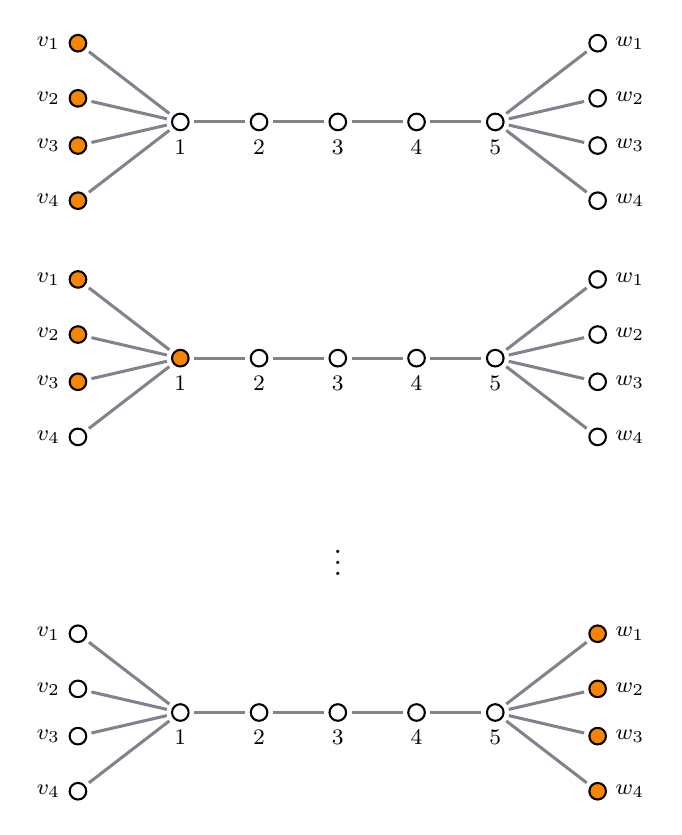
\begin{tikzpicture}
    
        \begin{scope}[]
            \draw (-2,0) node (1) [vertex,label=270:{\footnotesize $1$}] {};
            \draw (-1,0) node (2) [vertex,label=270:{\footnotesize $2$}] {};
            \draw (0,0) node (3) [vertex,label=270:{\footnotesize $3$}] {};
            \draw (1,0) node (4) [vertex,label=270:{\footnotesize $4$}] {};
            \draw (2,0) node (5) [vertex,label=270:{\footnotesize $5$}] {};
            \draw (-3.3,-1) node (6) [vertex,fill=naranja,label=180:{\footnotesize $v_4$}] {};
            \draw (-3.3,-0.3) node (7) [vertex,fill=naranja,label=180:{\footnotesize $v_3$}] {};
            \draw (-3.3,0.3) node (8) [vertex,fill=naranja,label=180:{\footnotesize $v_2$}] {};
            \draw (-3.3,1) node (9) [vertex,fill=naranja,label=180:{\footnotesize $v_1$}] {};
            \draw (3.3,-1) node (10) [vertex,label=0:{\footnotesize $w_4$}] {};
            \draw (3.3,-0.3) node (11) [vertex,label=0:{\footnotesize $w_3$}] {};
            \draw (3.3,0.3) node (12) [vertex,label=0:{\footnotesize $w_2$}] {};
            \draw (3.3,1) node (13) [vertex,label=0:{\footnotesize $w_1$}] {};

            \foreach \i/\j in{1/2,1/6,1/7,1/8,1/9,2/3,3/4,4/5,5/10,5/11,5/12,5/13} 
                \draw [edge,grisOscuro!75] (\i) to (\j);
        \end{scope}

        \begin{scope}[yshift=-3cm]
            \draw (-2,0) node (1) [vertex,fill=naranja,label=270:{\footnotesize $1$}] {};
            \draw (-1,0) node (2) [vertex,label=270:{\footnotesize $2$}] {};
            \draw (0,0) node (3) [vertex,label=270:{\footnotesize $3$}] {};
            \draw (1,0) node (4) [vertex,label=270:{\footnotesize $4$}] {};
            \draw (2,0) node (5) [vertex,label=270:{\footnotesize $5$}] {};
            \draw (-3.3,-1) node (6) [vertex,label=180:{\footnotesize $v_4$}] {};
            \draw (-3.3,-0.3) node (7) [vertex,fill=naranja,label=180:{\footnotesize $v_3$}] {};
            \draw (-3.3,0.3) node (8) [vertex,fill=naranja,label=180:{\footnotesize $v_2$}] {};
            \draw (-3.3,1) node (9) [vertex,fill=naranja,label=180:{\footnotesize $v_1$}] {};
            \draw (3.3,-1) node (10) [vertex,label=0:{\footnotesize $w_4$}] {};
            \draw (3.3,-0.3) node (11) [vertex,label=0:{\footnotesize $w_3$}] {};
            \draw (3.3,0.3) node (12) [vertex,label=0:{\footnotesize $w_2$}] {};
            \draw (3.3,1) node (13) [vertex,label=0:{\footnotesize $w_1$}] {};

            \foreach \i/\j in{1/2,1/6,1/7,1/8,1/9,2/3,3/4,4/5,5/10,5/11,5/12,5/13} 
                \draw [edge,grisOscuro!75] (\i) to (\j);
        \end{scope}


        \begin{scope}[]
            \node at (0,-5.5) {\large \vdots};
        \end{scope}

        \begin{scope}[yshift=-7.5cm]
            \draw (-2,0) node (1) [vertex,label=270:{\footnotesize $1$}] {};
            \draw (-1,0) node (2) [vertex,label=270:{\footnotesize $2$}] {};
            \draw (0,0) node (3) [vertex,label=270:{\footnotesize $3$}] {};
            \draw (1,0) node (4) [vertex,label=270:{\footnotesize $4$}] {};
            \draw (2,0) node (5) [vertex,label=270:{\footnotesize $5$}] {};
            \draw (-3.3,-1) node (6) [vertex,label=180:{\footnotesize $v_4$}] {};
            \draw (-3.3,-0.3) node (7) [vertex,label=180:{\footnotesize $v_3$}] {};
            \draw (-3.3,0.3) node (8) [vertex,label=180:{\footnotesize $v_2$}] {};
            \draw (-3.3,1) node (9) [vertex,label=180:{\footnotesize $v_1$}] {};
            \draw (3.3,-1) node (10) [vertex,fill=naranja,label=0:{\footnotesize $w_4$}] {};
            \draw (3.3,-0.3) node (11) [vertex,fill=naranja,label=0:{\footnotesize $w_3$}] {};
            \draw (3.3,0.3) node (12) [vertex,fill=naranja,label=0:{\footnotesize $w_2$}] {};
            \draw (3.3,1) node (13) [vertex,fill=naranja,label=0:{\footnotesize $w_1$}] {};

            \foreach \i/\j in{1/2,1/6,1/7,1/8,1/9,2/3,3/4,4/5,5/10,5/11,5/12,5/13} 
                \draw [edge,grisOscuro!75] (\i) to (\j);
        \end{scope}

        
    \end{tikzpicture}
    \caption{La gr\'afica $G$ utilizada como ejemplo del Teorema\ref{teo:diamFG}, 
    resaltando el movimiento de las $4$ fichas al pasar de un extremo de la 
    gr\'afica al otro}
\label{fig:ex-diamT}       
\end{figure}

Nuestro siguiente resultado muestra que algunas subgr\'aficas inducidas de las
gr\'aficas de fichas son productos cartesianos de algunas subgr\'aficas
inducidas de $G$.

\begin{teorema}
    \label{teo:PCartes}
    Sean $H_1, \dots, H_m$ subgr\'aficas inducidas de una gr\'afica $G$ tales
    que son ajenas dos a dos. Para todos los enteros $s_1, \dots, s_m$ tales que
    $1 \leq s_i \leq |V(H_i)|$ y $\Sigma s_i = k$, se tiene que $F_{s_1}(H_1)
    \square \cdots \square F_{s_m}(H_m)$ es una subgr\'afica inducida de
    $F_k(G)$.
\end{teorema}

\begin{proof}
    Sean $H_1, \dots, H_m$ subgr\'aficas inducidas de  $G$ y sean $s_1,
    \dots, s_m \in \mathbb{Z}$ como en el enunciado. Definimos el
    conjunto $L$ de los $k$-subconjuntos de $G$ que cumplen tener
    exactamente $s_i$ elementos de $H_i$, para $i \in \{1, \dots, m\}$,
    es decir $L = \{A \subseteq G \colon\ |A\cap H_1|=s_1 , |A \cap
    H_2|=s_2, \dots, |A \cap H_m|=m \}$. Observamos que, debido a  que
    $\Sigma s_i = k$, todo elemento de $L$ tiene cardinalidad $k$.
    Veamos que la subgr\'afica inducida de $F_k(G)$ por $L$, i.e. $F_k(G,L)$,
    es isomorfa a $F_{s_1}(H_1) \square \cdots \square F_{s_m}(H_m)$.
    Primero, analizamos el conjunto de v\'ertices de ambas
    gr\'afcias de fichas. Sea $A \in V(F_k(G,L))$, de tal manera que $A=\{a_1,
    \dots, a_{s_1}, b_1,\dots, b_{s_2}, \dots, m_1, \dots, m_{s_m}\}$.
    Por definici\'on tenemos que $|A \cap V(H_i)|= s_i$, para $i \in
    \{1, \dots, m\}$. Adem\'as sabemos que cada v\'ertice de
    $F_{s_i}(H_i)$ tiene cardinalidad $s_i$, para $i \in \{1, \dots,
    m\}$, por lo que tenemos que $A \in V(H_1) \times \cdots \times
    V(H_m)$. De manera an\'aloga, si tomamos $A \in V(H_1) \times \cdots
    \times V(H_m)$, $A = \{A'_1, A'_2, \dots, A'_m\}$ con $A'_i \in
    F_{s_i}(H_i)$. Entonces tenemos que $A \cap V(H_i) = A'_i$, por lo
    que $|A \cap V(H_i)|= s_i$, para toda $i \in \{1, \dots, m\}$.
    Adicionalmente, tenemos que $|A|= k$ puesto que $\Sigma s_i = k$.
    Por lo tanto tenemos que $A \in V(F_k(G,L))$.

    Ahora nos enfocamos en la relaci\'on entre las aristas de ambas
    gr\'aficas de fichas. Sean $B, C \in A \in V(F_k(G,L))$ tales que
    $BC \in E(F_k(G,L))$, en otras palabras, existen $b \in B$ y $c \in
    C$ tales que $B \triangle C = \{b, c\}$ y $bc \in E(G,L)$. Por
    definici\'on tenemos que $H_i \cap H_j = \varnothing$, con $i \neq
    j$, por lo que $b, c \in H_i$. Lo que significa que las fichas en
    $H_j$ est\'an est\'aticas, para todo $j \in \{1, \dots, m\} \setminus
    \{i\}$. Esto pasa si y s\'olo s\'i $BC$ es una arista en la
    subgr\'afica de fichas inducida por $H_i$. Como $H_i \cap H_j =
    \varnothing$, para $i \neq j$, entonces la subfr\'afica de fichas
    inducida por $H_i$ es isomora a $F_{s_i}(H_i)$. Al tener el resto de
    las fichas est\'aticas, tenemos que $BC \in E(F_{s_1}(H_1) \square
    \cdots \square F_{s_m}(H_m))$.

    Por lo tanto tenemos un isomorfismo entre $F_{s_1}(H_1) \square
    \cdots \square F_{s_m}(H_m)$ y $F_k(G,L)$ que es una subgr\'afica
    inducida de $F_k(G)$, por lo que tenemos que $F_{s_1}(H_1) \square
    \cdots \square F_{s_m}(H_m)$ es una subgr\'afica inducida de
    $F_k(G)$.
\end{proof}

La Figura\ref{fig:ex-cart}, exhibida a continuaci\'on, es un ejemplo sencillo
d\cref{teo:PCartes}. Del lado izquierdo de la figura tenemos una gr\'afica $G$,
resaltando dos subgr\'aficas inducidas ${\color{baige}\bf H_1}$ y
${\color{azulMetal}\bf H_2}$. El conjunto de v\'ertices de  y
${\color{azulMetal}\bf H_2}$  es $\{1,2,4,6\}$ mientras que el de
${\color{baige}\bf H_1}$ es $\{3\}$. Ahora, por un lado tenemos que $1\leq s_1
\leq |V(H_1)|$ por lo que $s_1 =1$. Por el otro lado $1\leq s_2 \leq |V(H_2)| =
4$ y, adem\'as, $s_1+s_2 = k =3$, por lo que $s_2 =2$. Del lado derecho de
\cref{fig:ex-cart} se muestra la gr\'afica $F_3(G)$, resaltando de
$\color{fushia} \bf rosa$ el producto carteciano $F_1(H_1) \square F_2(H_2)$.
Observamos que dicha gr\'afica es, en efecto, una subgr\'afica inducida de
$F_3(G)$.

\begin{figure}[ht!]
    \centering
       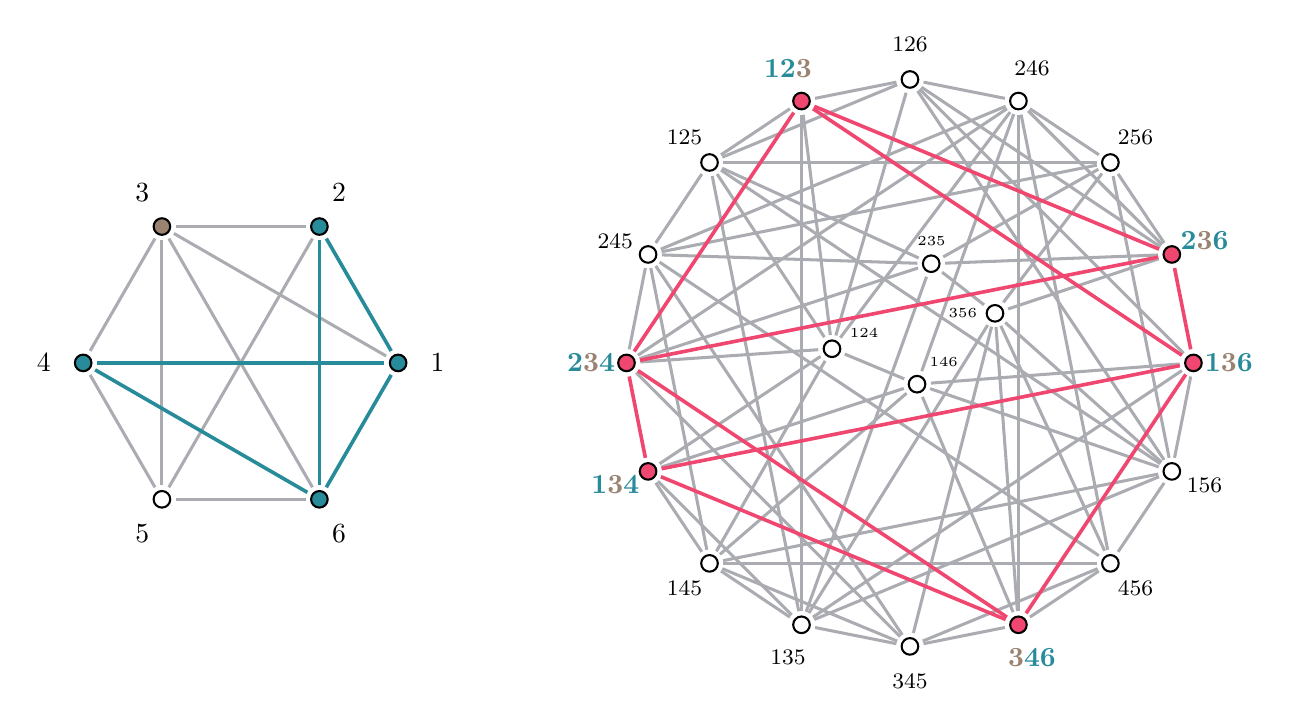
\begin{tikzpicture}
    
        \begin{scope}[xshift=-8.5cm]
            \foreach \i in {0,1,3,5}
                \draw ({(360/6)*\i}:2) node(\i)[wvertex,fill=azulMetal]{};
            \draw ({(360/6)*2}:2) node(2)[wvertex,fill=baige]{};
            \draw ({(360/6)*4}:2) node(4)[wvertex]{}; 
            \foreach \i in {0,...,5}
                \draw ({(360/6)*\i}:2.5) node(e0){\pgfmathparse{int(\i+1)}
               \pgfmathresult};
            \foreach \i/\j in {0/2,1/2,1/4,2/3,2/4,2/5,3/4,4/5}
                \draw [edge,grisOscuro!50] (\i) to (\j);
            
            \foreach \i/\j in {0/1,0/5,0/3,1/5,3/5}
                \draw [wedge,azulMetal] (\i) to (\j); 
            \end{scope}
        
        \begin{scope}[xshift=0cm,yshift=0cm,scale=0.9]
            \foreach \i in {0,1,5,8,9,13} 
                \draw ({(360/16)*\i}:4) node(\i)[wvertex,fill=fushia]{}; 
            \foreach \i in {2,3,4,6,7,10,11,12,14,15} 
                \draw({(360/16)*\i}:4) node(\i)[wvertex]{};
    
            \draw ({(360/16)*1}:4.5) node (e1) {{${\color{azulMetal}\bf 2}{\color{baige}\bf 3}{\color{azulMetal}\bf6}$}};
            \draw ({(360/16)*2}:4.5) node (e1) {{\footnotesize $256$}};
            \draw ({(360/16)*3}:4.5) node (e1) {{\footnotesize $246$}};
            \draw ({(360/16)*4}:4.5) node (e1) {{\footnotesize $126$}};
            \draw ({(360/16)*5}:4.5) node (e1) {{${\color{azulMetal}\bf12}{\color{baige}\bf 3}$}};
            \draw ({(360/16)*6}:4.5) node (e1) {{\footnotesize $125$}};
            \draw ({(360/16)*7}:4.5) node (e1) {{\footnotesize $245$}};
            \draw ({(360/16)*8}:4.5) node (e1) {{${\color{azulMetal}\bf2}{\color{baige}\bf 3}{\color{azulMetal}\bf4}$}};
            \draw ({(360/16)*9}:4.5) node (e1) {{${\color{azulMetal}\bf1}{\color{baige}\bf 3}{\color{azulMetal}\bf4}$}};
            \draw ({(360/16)*10}:4.5) node (e1) {{\footnotesize $145$}};
            \draw ({(360/16)*11}:4.5) node (e1) {{\footnotesize $135$}};
            \draw ({(360/16)*12}:4.5) node (e1) {{\footnotesize $345$}};
            \draw ({(360/16)*13}:4.5) node (e1) {{${\color{baige}\bf 3}{\color{azulMetal}\bf46}$}};
            \draw ({(360/16)*14}:4.5) node (e1) {{\footnotesize $456$}};
            \draw ({(360/16)*15}:4.5) node (e1) {{\footnotesize $156$}};
            \draw ({(360/16)*16}:4.5) node (e1) {{${\color{azulMetal}\bf1}{\color{baige}\bf 3}{\color{azulMetal}\bf6}$}};
    
            \draw (-1.1,0.2) node (17) [vertex,label=10:{\tiny $124$}] {};
            \draw (0.1,-0.3) node (18) [vertex,label=70:{\tiny $146$}] {};
            \draw (1.2,0.7) node (19) [vertex,label=180:{\tiny $356$}] {};
            \draw (0.3,1.4) node (20) [vertex,label=88:{\tiny $235$}] {};
            
            \foreach\i/\j in{0/4,0/11,0/15,0/18,1/2,1/3,1/4,1/19,1/20,2/3,2/6,
            2/7,2/15,2/19,2/20,3/4,3/7,3/8,3/13,3/14,3/17,3/18,4/5,4/6,4/15,4/17,
            5/6,5/11,5/17,6/7,6/11,6/15,6/17,6/20,7/8,7/10,7/12,7/14,7/20,8/12,
            8/17,8/20,9/10,9/11,9/17,9/18,10/11,10/12,10/14,10/15,10/17,10/18,
            11/12,11/15,11/19,11/20,12/13,12/14,12/19,13/14,13/18,13/19,14/15,
            14/19,15/18,15/19,17/18,19/20} 
               \draw [edge,grisOscuro!50] (\i) to (\j);

               \foreach \i/\j in {0/1,0/5,0/9,0/13,1/5,1/8,5/8,8/9,8/13,9/13}
               \draw [wedge,fushia] (\i) to (\j);
       \end{scope}

    \end{tikzpicture}
    \caption{Del lado izquierdo se muestra una gr\'afica $G$, donde se resaltan dos
    subgr\'aficas inducidas, ${\color{baige}\bf H_1}$ y ${\color{azulMetal}\bf
    H_2}$. Del lado derecho se muestra $F_3(G)$, donde se resalta su subgr\'afica
    inducida ${\color{fushia}\bf F_1(H_1) \square F_2(H_2)}$}
    \label{fig:ex-cart}
    \end{figure}

\newpage

\section{Trayectorias Internamente Ajenas}%
\label{sec:TrayIntAj}

El objetivo de este cap\'itulo es estudiar la relaci\'on de la conexidad entre
una gr\'afica y su gr\'afica de $k$-fichas. Para esto, empezaremos
enfoc\'andonos en determinar la cantidad de trayectorias internamente ajenas
entre un par de v\'ertices en una gr\'afica de fichas. Veremos que esta cantidad
est\'a relacionada con la conexidad de la gr\'afica original. Adem\'as, para
gr\'aficas con conexidad suficientemente grande, podemos encontrar un n\'umero
a\'un mayor de trayectorias internamente ajenas. Para llegar a estos resultados,
primero se necesitan demostrar dos lemas que nos ser\'an de utilidad.

\begin{lema}%
\label{lem:TrayIntAj-G-FG}
Sea $A$ un $k$-conjunto en la gr\'afica $G$ y $a, b \in V(G)$ tales que $a \in
A$ y $b \notin A$. Sea $A' = (A \setminus \{ a \}) \cup \{ b \}$. Si $P$ y $Q$
son $ab$-trayectorias internamente ajenas en $G$, entonces $A \xrightarrow[P]{}
A'$ y $A \xrightarrow[Q]{} A'$ son trayectorias internamente ajenas en
$F_{k}(G)$.
\end{lema}

\begin{proof}
    Primero, supongamos que $|V(P) \cap A| \geq 2$, con $V(P) \cap A = \{v_{1},
    v_{2}, \dots, v_{p}\}$, con $v_{1} = a$. Notemos que, si $k > p$, entonces
    $k-p$ fichas no est\'an sobre $P$, por lo que est\'an est\'aticas en todos
    los v\'ertices de $A \xrightarrow[P]{} A'$. Ahora, consideremos $R$ un
    v\'ertice interno de $A \xrightarrow[P]{} A'$. Por la observaci\'on anterior
    tenemos que  $|R \cap V(P)| = p$. Por construcci\'on de $A \xrightarrow[P]{}
    A'$, $R$ tiene una ficha en la trayectoria $(v_{p},b ]$. Entonces, $R$ no
    contiene al conjunto $\{v_{2}, \dots, v_{p}\}$. Por otro lado, como
    $\{v_{2}, \dots, v_{p}\}$ est\'a en $A \cap V(P)$, y $Q$ y $P$ son
    internamente ajenas, entonces $\{v_{2}, \dots, v_{p}\}$ est\'an est\'aticos
    en cada v\'ertice de $A \xrightarrow[Q]{} A'$. Por lo tanto tenemos que $A
    \xrightarrow[P]{} A'$ y $A \xrightarrow[Q]{}A'$ son trayectorias
    internamente ajenas. Al suponer que $|A \cap Q| \geq 2$, tenemos un caso
    an\'alogo al anterior.

    Ahora, supongamos que $|A \cap V(P)| = 1$ y $|A \cap V(Q)| = 1$, es decir,
    $A \cap V(P) = \{a\} = A \cap V(Q)$. Sin p\'erdida de generalidad suponemos
    que $P$ no es la arista $ab$. Entonces, tenemos que $P \setminus \{a,b\}
    \neq \varnothing$. Por lo tanto, tenemos que todo v\'ertice interno de $A
    \xrightarrow[P]{} A'$ tiene alg\'un v\'ertice de $P \setminus \{a, b\}$. Por
    otro lado, ya que $P$ y $Q$ son internamente ajenos y s\'olo comparten el
    v\'ertice $a$ con $A$, ning\'un v\'ertice interno de $A \xrightarrow[Q]{}
    A'$ tiene un v\'ertice de $P \setminus \{a, b\}$. Luego, cada v\'ertice
    interno de ambas trayectorias tiene intersecci\'on vac\'\i{}a con $A$.
    Concluimos que $A \xrightarrow[P]{} A'$ y $A \xrightarrow[Q]{} A'$ son
    internamente ajenas.
\end{proof}

Enseguida se presenta el siguiente lema t\'ecnico, que ser\'a necesario para
demostrar el resultado principal de esta secci\'on. 

\begin{lema}%
\label{lem:rb-bipGraph}
    Sea $H$ una gr\'afica bipartita completa con clases de color $Y$ y $Z$,
    donde $|Y|<|Z|$. Si las aristas de $H$ est\'an coloreadas de azul y rojo de
    manera que cada v\'ertice de $Y$ es incidente en a lo m\'as una arista roja,
    entonces $H$ tiene un conjunto $M$ de aristas azules tal que cada v\'ertice
    en $Y$ incide en exactamente una arista de $M$. Adem\'as, la uni\'on de
    aristas rojas y aristas de $M$ es ac\'\i{}clica.
\end{lema}

\begin{proof}
    Sea $H$ una gr\'afica bipartita completa con clases de color $Y$ y $Z$ como
    se especificaron, notemos que esta coloraci\'on no es propia. Demostramos el
    resultado por inducci\'on sobre $|Y|$. 

    Primero, supongamos que $Y=\{y\}$. Como $H$ es bipartita completa, existe
    una arista azul $e$ tal que $y$ es incidente en $e$.   Sea $M = \{ e \}$.
    Por otro lado, a lo m\'as existe una arista roja incidente en $y$, digamos
    $e'$. Entonces la uni\'on de aristas rojas y aristas en $M$ es $\{e, e'\}$,
    que no es un ciclo.

    Ahora supongamos que $|Y|>1$. Como tenemos que $|Y|<|Z|$, y hay a lo m\'as
    una arista roja incidente en cada v\'ertice de $Y$, entonces existe alg\'un
    $x \in Z$ tal que no tiene aristas rojas incidentes. Sea $v \in Y$ y sea
    $e$, en caso de existir, la arista roja incidente en $v$. Tomamos $H'=
    (H-v)-x$ con $R'$ el conjunto de aristas rojas de $H'$. Observamos que $Y' =
    Y- v$ y $Z'= Z- x$ son las clases de color de $H'$. Por hip\'otesis de
    inducci\'on, existe un conjunto $M'$ de aristas azules incidentes en $H'$
    tal que cada v\'ertice de $Y'$ incide exactamente en una arista de $M'$.
    Adem\'as $R'\cup M'$ es ac\'\i{}clico.
    
    En $H$, definimos $M = M'\cup \{xv\}$. Al tomar $x$ sin aristas rojas
    tenemos que $M$ cumple tener una arista azul por v\'ertice en $Y$. Tambi\'en
    definimos $R= R'\cup \{ e \}$, si es que existe $e$.  Dado que  $M'\cup R'$
    es ac\'\i{}clica y las aristas $\{vx\}$ y $e$, en caso de existir, no
    est\'an en $M'\cup R'$, entonces tenemos que $M \cup R$ es ac\'\i{}clica.
\end{proof}

\begin{figure}[ht!]
    \centering
       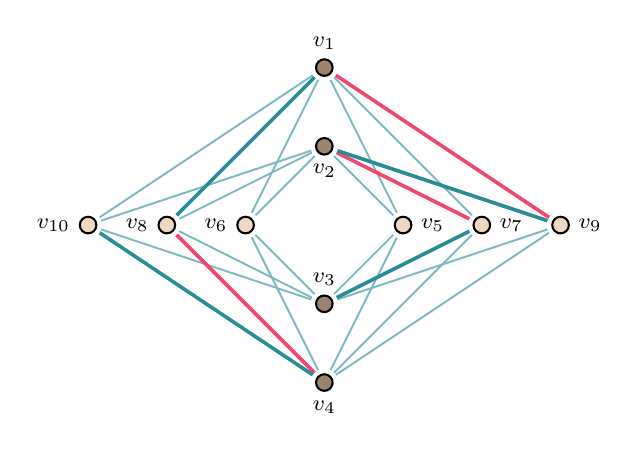
\begin{tikzpicture}
    
        \begin{scope}[xshift=-5.5cm]
            \draw (0,2) node (1) [vertex,fill=baige ,label=90:{\footnotesize $v_1$}] {};
            \draw (0,1) node (2) [vertex,fill=baige ,label=270:{\footnotesize $v_2$}] {};
            \draw (0,-1) node (3) [vertex,fill=baige ,label=90:{\footnotesize $v_3$}] {};
            \draw (0,-2) node (4) [vertex,fill=baige ,label=270:{\footnotesize $v_4$}] {};
            \draw (1,0) node (5) [vertex,fill=crema ,label=0:{\footnotesize $v_5$}] {};
            \draw (-1,0) node (6) [vertex,fill=crema ,label=180:{\footnotesize $v_6$}] {};
            \draw (2,0) node (7) [vertex,fill=crema ,label=0:{\footnotesize $v_7$}] {};
            \draw (-2,0) node (8) [vertex,fill=crema ,label=180:{\footnotesize $v_8$}] {};
            \draw (3,0) node (9) [vertex,fill=crema ,label=0:{\footnotesize $v_9$}] {};
            \draw (-3,0) node (10) [vertex,fill=crema ,label=180:{\footnotesize $v_{10}$}] {};

            \foreach \i/\j in{1/5,1/6,1/7,1/10,2/5,2/6,2/8,2/10,
            3/5,3/6,3/8,3/9,3/10,4/5,4/6,4/7,4/9} 
                \draw [nedge,azulMetal!60] (\i) to (\j);
            
            \foreach \i/\j in{1/9,2/7,4/8} 
                \draw [wedge,fushia] (\i) to (\j);
            
            \foreach \i/\j in{1/8,2/9,3/7,4/10} 
                \draw [wedge,azulMetal] (\i) to (\j);
        \end{scope}
        
    \end{tikzpicture}

\caption{Ejemplo de una bigr\'afica completa resaltando la uni\'on de aristas
${\color{fushia}rojas}$ y ${\color{azulMetal}azules}$ mencionadas en
\cref{lem:rb-bipGraph}.}
\label{fig:ex-rb-bioGraph}       
\end{figure}

Para aclarar \cref{lem:rb-bipGraph}, \cref{fig:ex-rb-bioGraph} muestra una
gr\'afica bipartita con bipartici\'on $({\color{crema}
\textbf{X}},{\color{baige} \textbf Y})$. Sea ${\color{azulMetal}M}$ el conjunto
de aristas azules mencionado en \cref{lem:rb-bipGraph}, resaltadas en figura.
Entonces tenemos que ${\color{azulMetal}M=\{v_1v_8, v_2v_9,v_3v_7,v_4v_{10}\}}$.
Notemos que todo v\'ertice en ${\color{baige}Y}$ tiene exactamente una arista en
${\color{azulMetal}M}$. Adem\'as, la uni\'on de las aristas de
${\color{azulMetal}M}$ y las aristas rojas, no forma un ciclo.

Ahora pasamos a demostrar el lema principal de esta secci\'on.

\begin{lema}%
\label{lem:TrayIntAj}
    Sea $G$ una gr\'afica $t$-conexa. Sean $A$ y $B$ v\'ertices de $F_{k}(G)$
    tales que $|A \triangle B| = 2$. Entonces hay $t$ $AB$-trayectorias
    internamente ajenas en $F_{k}(G)$. Adem\'as, si $t \geq k$, entonces hay
    $k(t- k + 1)$ $AB$-trayectorias internamente ajenas en $F_{k}(G)$.
\end{lema}

\begin{proof}
    Sea $G$ una gr\'afica $t$-conexa y sean $A$ y $B$ v\'ertices de $F_{k}(G)$
    tales que $|A \triangle B| = 2$. Primero buscamos probar el n\'umero de
    $AB$-trayectorias internamente ajenas en $F_{k}(G)$ es al menos $t$. 
    
    Sean $a \in A \setminus B$ y $b \in B \setminus A$ los v\'ertices en la
    diferencia sim\'etrica. Al ser $G$ una gr\'afica $t$-conexa, entonces por el
    Teorema General de Menger, existen $P_{1}, \dots, P_{t}$ $ab$-trayectorias
    internamente ajenas en $G$. Por lo tanto, por \cref{lem:TrayIntAj-G-FG},
    existen $A \xrightarrow[P_1]{}  B, \dots, A \xrightarrow[P_t]{}  B$
    $AB$-trayectorias internamente ajenas en $F_{k}(G)$. 

    Ahora buscamos demostrar que, si $t \geq k$, entonces el n\'umero de
    $AB$-trayectorias internamente ajenas en $F_{k}(G)$ es al menos $k(t- k
    +1)$. Si $t=k$, entonces tenemos que $k(t - k + 1) = t(t-t+1) = t$ por lo
    que tenemos el caso anterior. Por lo tanto consideramos  $t \geq k + 1$. Sea
    $\mathcal{P}$ un conjunto m\'aximo de $ab$-trayectorias internamente ajenas
    en $G$. Por el Teorema General de Menger sabemos que $|\mathcal{P}| \ge t$.
    Elegimos un conjunto $\mathcal{P}$ para el que ninguna trayectoria tenga
    cuerdas. Definimos a las trayectorias $P_{1}, \dots, P_{l}$ como aquellas en
    $\mathcal{P}$ que no intersectan a $A \cap B$ y $Q_{1}, \dots, Q_{s}$ las
    trayectorias en $\mathcal{P}$ que intersectan a $A \cap B$. Entonces $l + s
    = |\mathcal{P}| \ge t$.

    Definimos a $C$ como el conjunto de v\'ertices en $A \cap B$ que intersectan
    alg\'un $Q_i$, con $i \in \{1, \dots, s\}$. Observamos que, al ser $Q_1,
    \dots, Q_s$ internamente ajenas, entonces cada v\'ertice de $C$ est\'a en
    exactamente una $Q_i$, con $i \in \{1, \dots, s\}$. Definimos a $D$ como el
    conjunto de v\'ertices en $A \cap B$ que no intersecta a $Q_i$ alguna, con
    $i \in \{1, \dots, s\}$. Observamos que $C$ y $D$ inducen una partici\'on
    de $A \cap B$. Entonces, tenemos que $|A\cap B| = |C| + |D| = k-1$. Adem\'as
    podemos ver que $s \leq |C| \leq k-1$ y como $ t - s \leq l$, entonces $l
    \geq t -|C| = t- (k-1-|D|)$.

    Podemos separar las $AB$-trayectorias que consideramos en $F_{k}(G)$ en tres
    tipos. Los primeros dos tipos son las trayectorias obtenidas
    d\cref{lem:TrayIntAj-G-FG}, es decir, las trayectorias $A
    \xrightarrow[P_1]{}  B, \dots, A \xrightarrow[P_l]{}  B$ y $A
    \xrightarrow[Q_1]{}  B, \dots, A \xrightarrow[Q_s]{}  B$. Nombramos a estos
    tipos de $AB$-trayectorias trayectorias de tipo $P$ y de tipo $Q$,
    respectivamente. Notamos que, por como se defini\'o, toda $AB$-trayectoria
    de tipo $P$ no pasa por $A\cap B$, por lo que cada trayectoria de este tipo
    corresponde a la sucesi\'on de fichas obtenidas al mover la ficha de $a$ a
    trav\'es de $P_i$ hacia $b$, con $i \in \{1, \dots, l\}$.
    
    Las \'ultimas trayectorias a considerar son las del tipo $R$, que ahora
    construimos utilizando los vecinos de los v\'ertices en $A \cap B$. Primero
    consideramos $v \in C$, por lo que $v \in Q_i$ para un  $i \in \{1, \dots,
    s\}$. Definimos $Y_v = N_G(v) \setminus ((A \cap B) \cup V(Q_i))$. Dado que
    $G$ es una gr\'afica $t$-conexa, $d_G(v) \geq t$. A su vez, $|A \cap B| =k
    -1$ y $v \in (A \cap B) \setminus N_G(v)$. Por \'ultimo, como $Q_i$ no tiene
    cuerdas, $v$ s\'olo tiene dos vecinos en $Q_i$. Por lo tanto tenemos que
    $|Y_v| \geq t- (k-2)-2 = t-k$. 
    
    Ahora, sea $v \in D$ y definimos $Y_v = N_G(v) \setminus (A \cup B)$. Al ser
    $G$ una gr\'afica $t$-conexa, se cumple $d_G(v) \geq t$. Adem\'as tenemos
    que $|A \cup B| = k + 1$ y $v \in (A \cup B) \setminus N_G(v)$. Ahora,
    notemos que $(a, v, b)$ no es una trayectoria en $G$. \'Esto pues de lo
    contrario tendr\'iamos una trayectoria cuyo \'unico v\'ertice interno no
    est\'a en $P_i$ ni $Q_j$, con $i \in \{1, \dots, l\}$ y $j \in
    \{1, \dots, s\}$, por lo que la trayectoria no estar\'ia en $\mathcal{P}$.
    Por lo que concluimos que $a \notin N_G(v)$ o $b \notin N_G(v)$. Por lo
    tanto tenemos que $|Y_v| \geq t- (k-1) = t-k + 1$. Elegimos a $Y_v '$,
    alg\'un subconjunto de $Y_v$ con cardinalidad $t-k$ si $v \in C$ y $t- k+ 1$
    si $v \in D$. Notamos que $Y_v ' \neq \varnothing$ porque tomamos $t \geq k
    + 1$, adem\'as tenemos que $a, b \notin Y_v '$ por definici\'on. 

    Sea $H_v$ la gr\'afica bipartita completa con clases de colores $Y_v '$ y
    $\{1,\dots, l\}$. Definimos la siguiente coloraci\'on, si $y \in P_i$, para
    alg\'un $i \in \{1, \dots, l\}$ y $y \in Y_v '$, entonces coloreamos la
    arista $iy$ de rojo. Coloreamos el resto de las aristas de la gr\'afica de
    azul. Ahora veamos si la coloraci\'on definida cumple las hip\'otesis
    d\cref{lem:rb-bipGraph} Primero tenemos que por construcci\'on
    de los $P_i$, con $i \in \{1, \dots, l\}$, cada v\'ertice de $Y_v '$ est\'a
    en a lo m\'as un $P_i$, por lo que cada v\'ertice de $Y_v '$ incide en a lo
    m\'as una arista roja. Luego, notemos que $|\{1, \dots, l\}| = l  \geq t-k+
    1+ |D| > t-k + |D|$. Si $v \in D$, entonces $|D| \geq 1$ por lo que $l \geq
    t- k+1 = |Y_v '|$. Si $v \in C$, tenemos que $l \geq t-k = |Y_v '|$.
    Entonces podemos usar \cref{lem:rb-bipGraph} en $H_v$ con $Z=
    \{1, \dots, l\}$ y $Y = Y_v '$. Por lo tanto hay un conjunto $M_v$ de
    aristas azules tal que cada v\'ertice en $Y$ incide en exactamente una
    arista de $M_v$ y la uni\'on de aristas rojas y aristas de $M_v$ es
    ac\'\i{}clica. Notamos que $|M_v|=|Y|$.

    Usando $M_v$ construimos las trayectorias de tipo $R$ de la siguiente
    manera. Para cada $jx \in M_v$ defininimos $R\langle v, x \rangle$ como la
    trayectoria en $F_k(G)$ que corresponde a mover la ficha en $v$ hacia $x$,
    luego recorrer la trayectoria $A\setminus \{v\} \xrightarrow[P_j]{}
    (A\setminus \{v\})'$, donde $(A\setminus \{v\})' = (A\setminus \{v,a\})\cup
    \{b\}$, y por \'ultimo, mover la ficha de $x$ hacia $v$. Notemos que las
    fichas en $(A\cap B)\setminus \{v\}$ est\'an estacionarias. Adem\'as, cada
    v\'ertice en $R\langle v,x \rangle$ se conforma por $((A\cap B)\setminus
    \{v\}) \cup \{x\}$ y alg\'un v\'ertice $y \in P_i$.

    Falta ver que cada trayectoria de tipo $R$ es internamente ajena al resto de
    las trayectorias. Primero veamos que las trayectorias de tipo $R$ son
    internamente ajenas dos a dos. Supongamos que existen $R \langle v, x
    \rangle$ y $R\langle v',x' \rangle$ tales que $(v,x) \neq (v',x')$ pero
    comparten un v\'ertice interno. Entonces tenemos que $ix \in M_v$ y $i'x'\in
    M_{v'}$, con $i, i' \in \{1, \dots, l\}$. Por construcci\'on de las
    trayectorias de tipo $R$ tenemos que $((A\cap B)\setminus \{v\}) \cup \{x,
    y\} =((A\cap B)\setminus \{v'\}) \cup \{x', y'\}$ para alg\'un $y \in P_i$ y
    $y' \in P_{i'}$. Al tener $x'\in Y_{v'} '$, y ya que $((A \cap B )\setminus
    \{v\}) \cap Y_{v'}'= \varnothing$, tenemos que $x' \in \{x,y\}$.
    An\'alogamente, como $(A \cap B) \cap P_i = \varnothing$, tenemos que $y'\in
    \{x, y\}$. Por lo tanto tenemos $\{x,y\}= \{x',y'\}$, lo cual implica que
    $(A\cap B)\setminus \{v\} = (A\cap B)\setminus \{v'\}$, entonces $v = v'$.
    \'Esto implica que $ix, i'x' \in M_v$, pero por construcci\'on cada
    v\'ertice de $Y_v '$ es incidente en s\'olo una arista de $M_v$, por lo que
    $x \neq x'$ y $i \neq i'$. Como tenemos que $\{x, y\}=\{x', y'\}$, entonces
    $x=y'$ y $y=x'$. Entonces tenemos que $x \in P_{i'}$ y $x'\in P_i$, lo cual
    implica que $xi'$ y $x'i$ son aristas rojas en $H_v$. Por lo tanto tenemos
    el ciclo $(x, i, x', i)$ con aristas de color azul, rojo, azul, rojo
    respectivamente, lo cual es una contradicci\'on. As\'i pues, las
    trayectorias de tipo $R$ son internamente ajenas dos a dos.

    Ahora veamos que las trayectorias de tipo $R$ y las de tipo $P$ son
    internamente ajenas entre s\'i. Sean $R\langle v,x \rangle$ y $A
    \xrightarrow[P_i]{}  B$, para alg\'un $i \in \{1, \dots, l\}$, trayectorias
    en $F_k(G)$ de tipo $R$ y $P$, respectivamente. Por construcci\'on, $v$ no
    est\'a en v\'ertice interno alguno de $R \langle v,x \rangle$. Por otro
    lado, como $ v \in A\cap B$, entonces $v$ est\'a est\'atico en $A
    \xrightarrow[P_i]{}  B$, es decir, $v$ est\'a en cada v\'ertice de la
    trayectoria. Por lo tanto tenemos que las trayectorias $R\langle v,x
    \rangle$ y $A \xrightarrow[P_i]{}  B$, para alg\'un $i \in \{1, \dots, l\}$,
    son internamente ajenas.

    Por \'ultimo, veamos que las trayectorias de tipo $Q$ y las de tipo $R$ son
    internamente ajenas entre s\'i. Sean $R\langle v,x \rangle$ y $A
    \xrightarrow[Q_i]{}  B$, para alg\'un $i \in \{1, \dots, s\}$, trayectorias
    en $F_k(G)$ de tipo $R$ y $Q$, respectivamente. Sea $jx$ arista en $M_v$,
    con $j \in \{1, \dots, l\}$, entonces $x \notin P_j$. Si tomamos $v \notin
    Q_i$, entonces $v$ est\'a est\'atico en $A \xrightarrow[Q_i]{} B$, es decir,
    est\'a en cada v\'ertice de la trayectoria. Por otro lado, por
    construcci\'on tenemos que $v$ no est\'a en los v\'ertices internos de $R
    \langle v, x \rangle$. Por lo tanto las trayectorias son internamente
    ajenas. Ahora consideramos el caso en el que $v \in Q_i$, es decir $v \in
    C$. Por como definimos $R \langle v,x \rangle$, $x$ est\'a en cada
    v\'ertice interno de la trayectoria. Por otro lado, como $x \in Y_v'$, y por
    construcci\'on, tenemos que $Y_v ' \cap ((A\cap B) \cup Q_i) = \varnothing$,
    entonces $x \notin ((A \cap B) \cup Q_i)$. Por definici\'on, cada v\'ertice
    de $A \xrightarrow[Q_i]{}  B$ est\'a contenido en $((A \cap B) \cup Q_i)$,
    entonces $x$ no est\'a en los v\'ertices internos de $A \xrightarrow[Q_i]{}
    B$. Por lo tanto tenemos que las trayectorias $R \langle v,x \rangle$ y $A
    \xrightarrow[Q_i]{}  B$ son internamente ajenas.

    Tenemos que hay $l$ y $s$ trayectorias de tipo $P$ y $Q$ respectivamente.
    Adem\'as, para cada $v \in C$ hay $t-k$ trayectorias de tipo $R$ y para cada
    $v \in D$ hay $t-k+1$ trayectorias de tipo $R$. Entonces en $F_k(G)$ hay $l+
    s+ |C|(t-k)+ |D|(t-k +1) = l + s + (|C| + |D|)(t-k) + |D| = l + s +
    (|k-1)(t-k) + |D|$ trayectorias internamente ajenas. Despejando tenemos que
    $l + s + (k-1)(t-k) + |D| \geq t+ (k-1)(t-k) = k (t -k +1)$. Por lo tanto el
    n\'umero de $AB$-trayectorias en $F_k(G)$ es al menos $k(t-k+1)$.

\end{proof}

Con esto queda demostrado el resultado principal de esta secci\'on. Para
intentar ejemplificar los tres tipos de trayectorias mencionados en
\cref{lem:TrayIntAj}, \cref{fig:ex-tok-path}, a continuaci\'on mostrada, exhibe
una gr\'afica $G$ del lado izquierdo y su gr\'afica de $3$-fichas del lado
derecho. Ahora construimos una trayectoria de cada tipo. Consideramos
${\color{baige}A= \{1,2,3\}}$ y ${\color{baige}B=\{2,3,5\}}$ los v\'ertices en
$F_3(G)$ sobre los que veremos los distintos tipos de trayectorias internamente
ajenas. Tenemos que ${\color{baige}A\triangle B=\{1,5\}}$ y $A\cap B=\{2,3\}$
por lo que usamos $15$-trayectorias para encontrar las trayectorias de tipo $P$
y las de tipo $Q$, de manera que las de tipo $P$ no tienen a $2$ ni a $3$ como
v\'ertice interno y las de tipo $Q$ tienen a ambos como v\'ertices internos,
recordando que $A\cap B=\{2,3\}$. Tomamos ${\color{naranja}P_1=(1,4,5)}$ y
${\color{fushia}Q_1(1,2,3,5)}$. Ahora tomamos ${\color{fushia}2} \in C$ y su
vecino ${\color{menta}x\notin P_1}$, en este caso $x=6$. De esta manera tenemos
la trayectoria del tercer tipo
\[
    {\color{verdeAzulado}R_1=(\{1,2,3\}.\{1,3,6\}\{1,4,6\}\{1,5,6\}\{2,5,6\}
    \{3,5,6\}\{2,3,5\})}.
\]


\begin{figure}[ht!]
\centering
   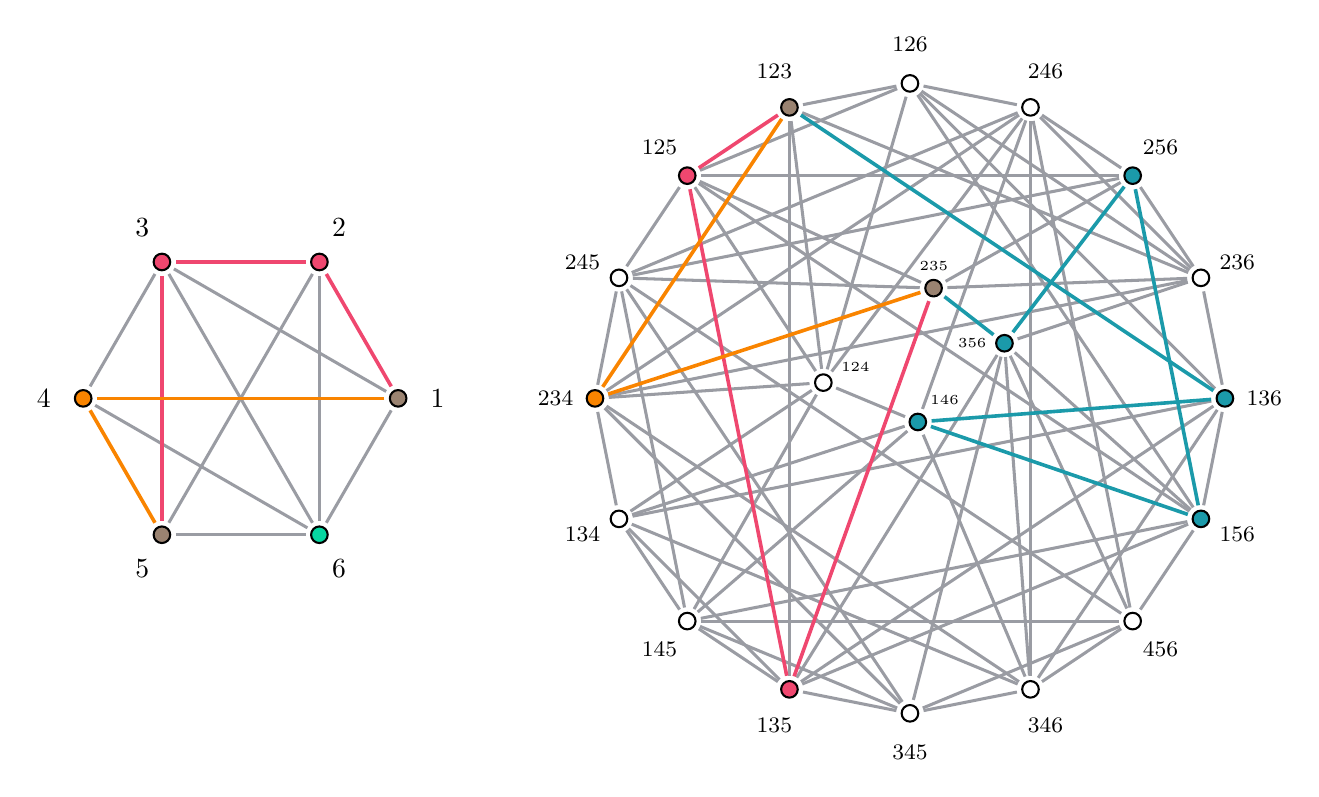
\begin{tikzpicture}

    \begin{scope}[xshift=-8.5cm]
        
       
        \foreach \i in {0,4}
            \draw ({(360/6)*\i}:2) node(\i)[wvertex,fill=baige]{};
        \foreach \i in {1,2}
            \draw ({(360/6)*\i}:2) node(\i)[wvertex,fill=fushia]{};
        \draw ({(360/6)*3}:2) node(3)[wvertex,fill=naranja]{};
        \draw ({(360/6)*5}:2) node(5)[wvertex,fill=menta]{}; 
        \foreach \i in {0,...,5}
            \draw ({(360/6)*\i}:2.5) node(e0){\pgfmathparse{int(\i+1)}
           \pgfmathresult};
        \foreach \i/\j in {0/2,0/5,1/4,1/5,2/3,2/5,3/5,4/5}
            \draw [edge,grisOscuro!60] (\i) to (\j);
        \foreach \i/\j in {0/1,1/2,2/4}
            \draw [wedge,fushia] (\i) to (\j);
        \foreach \i/\j in {0/3,3/4}
            \draw [wedge,naranja] (\i) to (\j);
        
        \end{scope}
    
    \begin{scope}[xshift=0cm,yshift=0cm,scale=1]

        \foreach \i in {6,11} 
            \draw ({(360/16)*\i}:4) node(\i)[wvertex,fill=fushia]{}; 
        \foreach \i in {0,2,15} 
            \draw ({(360/16)*\i}:4) node(\i)[wvertex,fill=verdeAzulado]{}; 
        
        \draw ({(360/16)*5}:4) node(5)[wvertex,fill=baige]{};
        \draw ({(360/16)*8}:4) node(8)[wvertex,fill=naranja]{};     
        \foreach \i in {1,3,4,7,9,10,12,13,14} 
            \draw({(360/16)*\i}:4) node(\i)[wvertex]{};

        \draw ({(360/16)*1}:4.5) node (e1) {{\footnotesize $236$}};
        \draw ({(360/16)*2}:4.5) node (e1) {{\footnotesize $256$}};
        \draw ({(360/16)*3}:4.5) node (e1) {{\footnotesize $246$}};
        \draw ({(360/16)*4}:4.5) node (e1) {{\footnotesize $126$}};
        \draw ({(360/16)*5}:4.5) node (e1) {{\footnotesize $123$}};
        \draw ({(360/16)*6}:4.5) node (e1) {{\footnotesize $125$}};
        \draw ({(360/16)*7}:4.5) node (e1) {{\footnotesize $245$}};
        \draw ({(360/16)*8}:4.5) node (e1) {{\footnotesize $234$}};
        \draw ({(360/16)*9}:4.5) node (e1) {{\footnotesize $134$}};
        \draw ({(360/16)*10}:4.5) node (e1) {{\footnotesize $145$}};
        \draw ({(360/16)*11}:4.5) node (e1) {{\footnotesize $135$}};
        \draw ({(360/16)*12}:4.5) node (e1) {{\footnotesize $345$}};
        \draw ({(360/16)*13}:4.5) node (e1) {{\footnotesize $346$}};
        \draw ({(360/16)*14}:4.5) node (e1) {{\footnotesize $456$}};
        \draw ({(360/16)*15}:4.5) node (e1) {{\footnotesize $156$}};
        \draw ({(360/16)*16}:4.5) node (e1) {{\footnotesize $136$}};

        \draw (-1.1,0.2) node (17) [vertex,label=10:{\tiny $124$}] {};
        \draw (0.1,-0.3) node (18) [vertex,fill=verdeAzulado ,label=70:{\tiny $146$}] {};
        \draw (1.2,0.7) node (19) [vertex,fill=verdeAzulado ,label=180:{\tiny $356$}] {};
        \draw (0.3,1.4) node (20) [vertex,fill=baige ,label=88:{\tiny $235$}] {};
        
        \foreach\i/\j in{0/1,1/2,2/3,3/4,4/5,6/7,7/8,8/9,9/10,10/11,
           11/12,12/13,13/14, 14/15, 15/0} 
           \draw [edge,grisOscuro!60] (\i) to (\j);
        \foreach\i/\j in{0/4,0/11,0/13,1/3,1/4,1/5,2/6,2/7,3/7,3/8,
        4/6,4/15,6/15,7/10,7/12,8/12,8/13,9/11,9/13,10/12,10/14,10/15,
        11/15,12/14} 
           \draw [edge,grisOscuro!60] (\i) to (\j);
        \foreach \i/\j in{1/8,3/13,3/14,5/11,7/14,9/0,9/18,17/3,17/4,17/5,17/6,
        17/8,17/9,17/10,17/18,3/18,18/10,18/13,19/1,19/11,19/12,
        19/13,19/14,19/15,20/1,20/2,20/6,20/7}
          \draw [edge,grisOscuro!60] (\i) to (\j);
        \foreach\i/\j in{5/6,6/11,11/20} 
           \draw [wedge,fushia] (\i) to (\j);
        \foreach\i/\j in{5/8,8/20} 
           \draw [wedge,naranja] (\i) to (\j);
        \foreach\i/\j in{5/0,0/18,18/15,15/2,2/19,19/20} 
          \draw [wedge,verdeAzulado] (\i) to (\j);
        
   \end{scope}

        

\end{tikzpicture}
\caption{Ejemplo de una gr\'afica $G$ y su gr\'afica de $3$-fichas resaltando
las trayectorias internamente ajenas de ${\color{baige}A}$ y
${\color{baige}B}$.}
\label{fig:ex-tok-path}
\end{figure}

\newpage

\section{Conexidad}%
\label{sec:conexidad}

Pasamos a enfocarnos en la conexidad de las gr\'aficas de fichas. Con ayuda de
los resultados encontrados en las secciones anteriores, esta secci\'on buscamos
estudiar la relaci\'on entre la conexidad de una gr\'afica y su gr\'afica de
$k$-fichas.  El siguiente teorema nos muestra la relaci\'on buscada.

\begin{teorema}%
\label{teo:FG-t-conexa}
    Sea $G$ una gr\'afica $t$-conexa. Entonces $F_{k}(G)$ es $t$-conexa para
    todo $k>1$
\end{teorema}
        
\begin{proof}
Primero, observamos que $A$ y $B$ son v\'ertices adyacentes en $F_k(G)$ si y
s\'olo si $V(G) \setminus A$ y $V(G)\setminus B$ son adyacentes en $F_{n-k}(G)$.
Entonces tenemos que $F_k(G) \cong F_{n-k}(G)$. Por lo tanto asumimos sin
p\'erdida de generalidad que $k \leq \frac{n}{2}$.

Sea $\mathcal{C}$ un m\'inimo corte por v\'ertices de $F_k(G)$. Basta
demostrar que $|\mathcal{C}| \geq t$. Definimos $A$ y $B$ como los v\'ertices en
distintas componentes de $F_k(G)- \mathcal{C}$ tales que $|A \triangle B|$ es
m\'inimo.

Si $|A \triangle B| = 2$, entonces por \cref{lem:TrayIntAj}
tenemos que hay $t$ $AB$-trayectorias internamente ajenas en $F_k(G)$. Por lo
que tenemos que $|\mathcal{C}| \geq t$.

Ahora consideramos $|A \triangle B| = 2r \geq 4$. Definimos $A \setminus B
=\{a_1, \dots, a_r\}$ y $B \setminus A =\{b_1, \dots, b_r\}$. Tambi\'en
definimos $A_{i,x} = A\setminus \{a_i\} \cup \{x\}$ y $B_{j,x} = B\setminus
\{b_j\} \cup \{x\}$ para cada $i \in \{1, \dots, r\}$ y $x \in V(G)\setminus
(A\cup B)$. Supongamos que para algunos $i, j$ y $x$ tenemos que $A_{i,x} \notin
\mathcal{C}$ y $B_{j,x} \notin \mathcal{C}$. Como $A \triangle A_{i,x} = \{a_i,
x\}$, entonces tenemos que $|A \triangle A_{i,x}|< |A \triangle B|$ por lo que
$A$ y $A_{i,x}$ est\'an en la misma componente de $F_k(G)- \mathcal{C}$.
An\'alogamente tenemos que  $B$ y $B_{j,x}$ est\'an en la misma componente de
$F_k(G)-\mathcal{C}$

Luego nos fijamos en que $A_{i,x} \triangle B_{j,x} = (A \triangle B) \setminus
\{a_i, b_j\}$. Por lo que $|A_{i,x} \triangle B_{j,x}| = 2(r-1)$. As\'i
tenemos que $A_{i,x}$ y $B_{j,x}$ est\'an en la misma componente de $F_k(G)-
\mathcal{C}$. Pero tenemos que $A$ y$A_{i,x}$ est\'an en la misma componente, de
$F_K(G) - \mathcal{C}$, de igual manera que $B$ y $B_{j,x}$. Por lo tanto $A$ y
$B$ est\'an en la misma componente de $F_k(G)- \mathcal{C}$. Esto es una
cotradicci\'on pues tomamos a $A$ y $B$ en distintas componentes, lo que implica
que $A_{i,x}$ o $B_{j,x}$ est\'a en $\mathcal{C}$, para todas las $i,j$ y $x$.

Por lo anterior tenemos que, para cada $x \in V(G)\setminus (A \cup B)$,
$\mathcal{C}$ tiene todos los $\{A_i,x \colon\  i \in \{1, \dots, r\}\}$ o todos los
$\{B_j,x \colon\ j \in \{1, \dots, r\}\}$. Dado que $|A\cup B|=k +r$, sabemos que
$\mathcal{C}$ tiene al menos $r(n-k-r)$ v\'ertices.

Ahora definimos $A_{i,j} = (A\setminus \{a_i\}) \cup \{b_j\}$ y $B_{i,j} =
(B\setminus \{b_i\}) \cup \{a_j\}$, para toda $ i, j \in \{1, \dots, r\}$.
Notamos que hay $2r^2$ de estos conjuntos. Ahora supongamos que $A_{i,j} \notin
\mathcal{C}$, para algunos $ i, j \in \{1, \dots, r\}$. Entonces tenemos que $A
\triangle A_{i,j} = \{a_i, b_j\}$. Entonces $A$ y $A_{i,j}$ est\'an en la misma
componente de $F_k(G)- \mathcal{C}$. Por otro lado, $|B \triangle A_{i,j}| = 2
(r-1)$, por lo que $B$ y $A_{i,j}$ est\'an en la misma componente de $F_k(G) -
\mathcal{C}$. Por lo tanto tenemos que $A$ y $B$ est\'an en la misma componente
de $F_k(G)-\mathcal{C}$, lo cu\'al nos lleva a la misma contradicci\'on que el
caso anterior. Por lo tanto tenemos que $A_{i,j} \in \mathcal{C}$ para toda $i,
j \in \{1, \dots, r\}$. De manera an\'aloga $B_{i,j} \in \mathcal{C}$. Por lo
tanto tenemos que $\mathcal{C}$ tiene $2r^2$ v\'ertices, adem\'as de los del
caso anterior.

As\'i, tenemos que $|\mathcal{C}|\geq r(n-k-r)+2r^2 = r(n-k) + r^2$, pero $r
\geq 2$ y $k \leq \frac{n}{2}$, por lo que tenemos que $|\mathcal{C}| \geq
r(n-k)+r^2 > r(n-k) \geq 2(n-k) \geq n >t$. Por lo tanto $|\mathcal{C}|>t$.
\end{proof} 

Para ejemplificar \cref{teo:FG-t-conexa} utilizaremos las gr\'aficas de
\cref{fig:ex-tConect}. Nos fijamos que $G$, mostrada del lado izquierdo, es una
gr\'afica $4$-conexa y su gr\'afica de $2$-fichas, mostrada del lado derecho, es
$8$-conexa. En la figura se muestra los conjuntos de corte
${\color{naranja}\{1,3,5,6\}}$ y
${\color{fushia}\{\{1,2\},\{1,3\},\{1,5\},\{1,6\},\{2,4\},\{3,5\},\{3,6\},\{5,6\}\}}$
para $G$ y $F_2(G)$, respectivamente. Adem\'as, utilizando
\cref{fig:ex-tok-path}, podeos ver que $F_3(G)$ es $9$-conexa. Por lo tanto
tenemos que $F_2(G)$ y $F_3(G)$ son gr\'aficas $4$-conexas.

\begin{figure}[ht!]
    \centering
       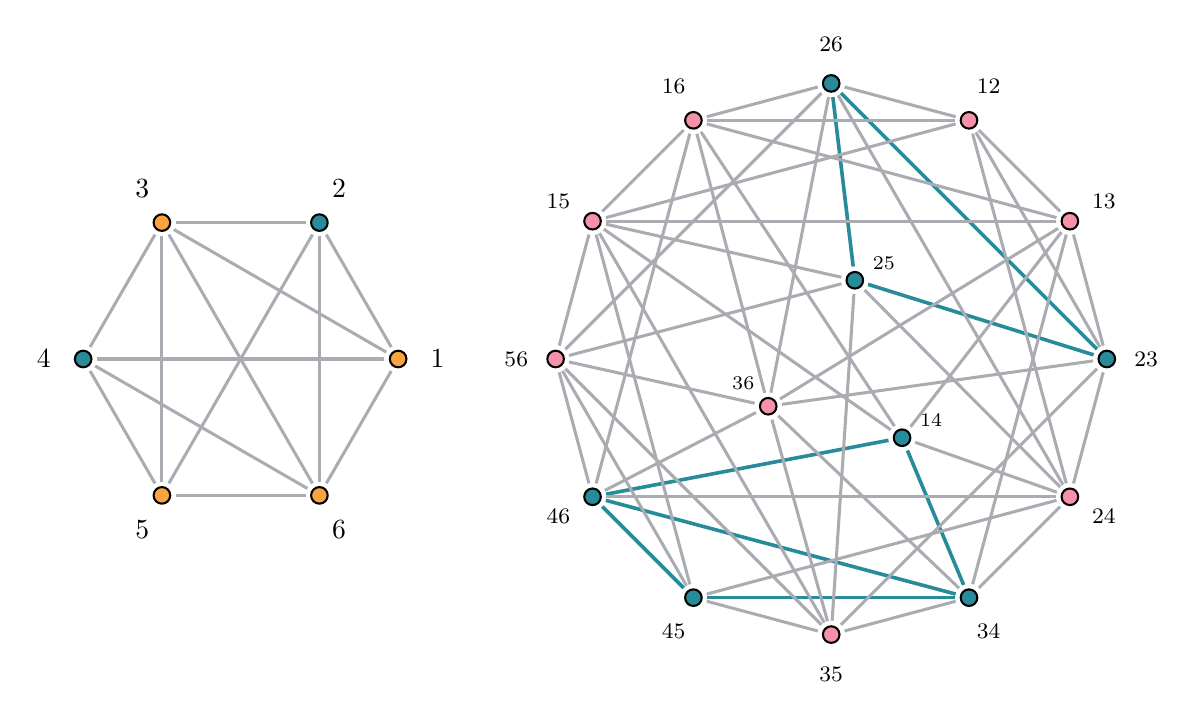
\begin{tikzpicture}
    
        \begin{scope}[xshift=-8.5cm]
            \foreach \i in {1,3}
                \draw ({(360/6)*\i}:2) node(\i)[vertex,fill=azulMetal]{};

            \foreach \i in {0,2,4,5}
                \draw ({(360/6)*\i}:2) node(\i)[vertex,fill=naranja!75]{};

                
            \foreach \i in {0,...,5}
                \draw ({(360/6)*\i}:2.5) node(e0){\pgfmathparse{int(\i+1)}
               \pgfmathresult};

            \foreach \i/\j in {0/1,0/2,0/3,0/5,1/2,1/4,1/5,2/3,2/4,2/5,3/4,3/5,4/5}
                \draw [edge,grisOscuro!50] (\i) to (\j);
            
            \end{scope}
        
        \begin{scope}[xshift=-1cm,yshift=0cm,scale=1]
        
            \foreach \i in{0,3,7,8,10} \draw ({(360/12)*\i}:3.5)
            node(\i)[wvertex,,fill=azulMetal]{};

            \foreach \i in{1,2,4,5,6,9,11} \draw ({(360/12)*\i}:3.5)
            node(\i)[wvertex,fill=fushia!60]{};
    
            \draw ({(360/12)*1}:4) node (e1) {{\footnotesize $13$}};
            \draw ({(360/12)*2}:4) node (e1) {{\footnotesize $12$}};
            \draw ({(360/12)*3}:4) node (e1) {{\footnotesize $26$}};
            \draw ({(360/12)*4}:4) node (e1) {{\footnotesize $16$}};
            \draw ({(360/12)*5}:4) node (e1) {{\footnotesize $15$}};
            \draw ({(360/12)*6}:4) node (e1) {{\footnotesize $56$}};
            \draw ({(360/12)*7}:4) node (e1) {{\footnotesize $46$}};
            \draw ({(360/12)*8}:4) node (e1) {{\footnotesize $45$}};
            \draw ({(360/12)*9}:4) node (e1) {{\footnotesize $35$}};
            \draw ({(360/12)*10}:4) node (e1) {{\footnotesize $34$}};
            \draw ({(360/12)*11}:4) node (e1) {{\footnotesize $24$}};
            \draw ({(360/12)*12}:4) node (e1) {{\footnotesize $23$}};
            \draw (0.3,1) node (13) [vertex,,fill=azulMetal, label=10:{\scriptsize $25$}] {};
            \draw (0.9,-1) node (14) [vertex,fill=azulMetal, label=10:{\scriptsize $14$}] {};
            \draw (-0.8,-0.6) node (15) [vertex,fill=fushia!60, label=120:{\scriptsize $36$}] {};
          
            
            \foreach\i/\j in{0/3,0/13,3/13,7/10,7/14,8/10,7/8,10/14} 
            \draw [wedge,azulMetal] (\i) to (\j);

            \foreach\i/\j in{0/1,1/2,1/4,1/5,1/10,1/14,
            1/15,2/3,0/2,2/4,2/5,2/11,4/5,4/7,4/14,4/15,3/4,5/6,6/7,3/6,5/8,5/9,5/13,
            5/14,6/8,6/9,6/13,6/15,8/9,9/10,10/11,0/9,9/13,9/15,0/11,3/11,7/11,8/11,
            11/13,11/14,0/15,3/15,7/15,10/15} 
               \draw [edge,grisOscuro!50] (\i) to (\j);
           
            \end{scope}

    \end{tikzpicture}
    \caption{Cortes m\'inimos en $G$ y en $F_2(G)$.}
    \label{fig:ex-tConect}
    \end{figure}

Por \'ultimo, el siguiente teorema presenta una mejor cota para gr\'aficas
suficientemente conexas y suficientemente grandes.

\begin{teorema}%
    \label{teo:FG_k(t- k+ 1)-conexa}
        Sea $G$ una gr\'afica $t$-conexa con $t \ge k$ y $n \ge \frac{1}{2} kt$.
        Entonces $F_{k}(G)$ es $k (t- k+ 1)$-conexa.
    \end{teorema}

    \begin{proof}
        Sea $\mathcal{C}$ un corte por v\'ertices m\'inimo de $F_k(G)$. Sean
        $A$ y $B$ v\'ertices en distintas componentes de $F_k(G)- \mathcal{C}$
        tales que $|A \triangle B|$ es m\'inima.

        Si $|A \triangle B| = 2$, entonces por \cref{lem:TrayIntAj} tenemos que
        $F_k(G)$ tiene $k (t- k+ 1)$ $AB$-trayectorias. Por lo que tenemos que
        $|\mathcal{C}| \geq k (t- k+ 1)$.

        Ahora veamos el caso en el que $|A \triangle B| = 2r \ge 4$. Utilizando
        la desigualdad que se utiliza al final de la demostraci\'on
        d\cref{teo:FG-t-conexa} tenemos que $|\mathcal{C}| \ge r(n-k-r)+2r^2$. Dado
        que $r \ge 2$ y $n \ge \frac{1}{2}kt$, entonces tenemos que
        $|\mathcal{C}| \ge r(n-k-r)+2r^2 \ge 2 (n- k -2) + 8 \ge tk - 2k+ 4$.
        Observamos que $k^2 -3k + 4 \ge 0$ para toda $k \ge 1$. Entonces tenemos
        que $-2k+4 \ge -k^2 + k$, esto implica que $kt -2k +4 \ge kt - k^2 + k =
        k (t - k +1)$. Entonces tenemos que $|\mathcal{C}| \ge tk -2k +4 \ge
        k(t-k+1)$. Por lo tanto $F_k(G)$ es $k(t-k+1)$-conexa.
    \end{proof}
\chapter{Clanes y N\'umero Crom\'atico}%
\label{cap:Clique-ChromNum}
Los clanes y el n\'umero crom\'atico de una gr\'afica son partes importantes en
el estudio de las gr\'aficas. En este cap\'itulo estudiaremos un poco el c\'omo
se ven los clanes en las gr\'aficas de fichas. De igual manera, estudiaremos el
n\'umero crom\'atico de una gr\'afica de fichas en relaci\'on a la gr\'afica
original. Las proposiciones de ambas secciones salen del art\'iculo
\textit{Token graphs} \cite{fabilaToken}. 

\section{Clanes}%
\label{sec:clanes}

Esta secci\'on est\'a enfocada en los clanes de las gr\'aficas de fichas. Se
dar\'a una caracterizaci\'on de los clanes, adem\'as de una manera de encontrar
el n\'umero de clan en las gr\'aficas de fichas. Las demostraciones de esta
secci\'on salen del art\'iculo \textit{Token graphs} \cite{fabilaToken}, con
excepci\'on del \cref{coro:numClan}.

Empezamos con la caracterizaci\'on de los clanes. Para esto, se necesita el
siguiente lema, por lo que proseguimos a demostrarlo.

\begin{lema}%
\label{lem:K3}
    Sean $G$ una gr\'afica y $F_k(G)$ su gr\'afica de $k$-fichas. Si $A$, $B$ y
    $C$ son v\'ertices en $F_k(G)$, tales que son adyacentes dos a dos, entonces
    se cumple s\'olo una de las siguientes relaciones: $B \cap C \subset A$ o $A
    \subset B \cup C$.
\end{lema}

\begin{proof}
    Primero, supongamos que existen $A$, $B$, $C$ v\'ertices en $F_k(G)$, tales
    que son adyacentes dos a dos y cumplen $B \cap C \not\subset A$ y $A
    \not\subset B \cup C$, entonces existen los v\'ertices  $a \in A \setminus
    (B \cup C)$ y $b \in (B \cap C)\setminus A$. Notamos que $b \in B \setminus
    A$ y $b \in C \setminus A$. De manera an\'aloga, tenemos que $a \in A
    \setminus B$ y $a \in A \setminus C$. Por otro lado, sabemos que $A$ y $B$
    son adyacentes en $F_k(G)$, al igual que $A$ y $C$. Por lo tanto, tenemos
    que $A \triangle B = \{a,b\}$ y $A \triangle C = \{a, b\}$. As\'i pues, $(B
    \cup C \cup \{a\})\setminus \{b\} \subseteq A$. Pero $B$ y $C$ son
    adyacentes en $F_k(G)$, por lo que $|B \cup C| = k+1$. Luego, $|A| \geq
    k+1$, lo cu\'al es una contradicci\'on pues $A \in V (F_k(G))$. 

    Ahora, supongamos que existen $A$, $B$ y $C$ v\'ertices en $F_k(G)$ que son
    adyacentes dos a dos y cumplen $A \subset B \cup C$ y $B \cap C \subset A$.
    Como $B$ y $C$ son adyacentes, entonces tenemos que $B \triangle C =
    \{b,c\}$ con $b \in B$ y $c \in C$. Adem\'as, tenemos que $|B \cap C| = k-1$
    y $|B \cup C| = k +1$. Notamos que $B \cup C = (B\cap C) \cup \{b,c\}$. Por
    otro lado, dado que $|A|=k$ y $B \cap C \subset A$, tenemos que existe $a
    \in A$ tal que $A = (B \cap C) \cup \{a\}$. Adicionalmente, $A \subset B
    \cup C$, por lo que $a \in \{b, c\}$. Por eso, tenemos que $A = (B \cap C)
    \cup \{b\}$ o $A = (B \cap C) \cup \{c\}$, es decir, $A = B$ o $A=C$, lo
    cu\'al es una contradicci\'on. Por lo tanto, $B \cap C \subset A$ o $A
    \subset B \cup C$.
\end{proof}

Ahora, teniendo en cuenta \cref{lem:K3}, pasamos a demostrar el siguiente
teorema de caracterizaci\'on de los clanes en gr\'aficas de fichas.

\begin{teorema}
\label{teo:clanG-clanFG}
    Sea $F_k(G)$ la gr\'afica de $k$-fichas de una gr\'afica $G$. Si $X$ es un
    conjunto de v\'ertices de $F_k(G)$, entonces $X$ es un clan de $F_k(G)$ si y
    s\'olo si hay un clan $K$ de $G$ y un conjunto $S \subseteq V(G)$, tales que
    $K \cap S = \varnothing$ y pasa uno de los siguientes casos:
        \begin{enumerate}
            \item $X = \{S \cup \{v\}\colon\ v \in K\}$ y $|S| = k-1$
            \item $X = \{(S\cup K) \setminus \{v\}\colon\ v \in K \}$ y $|S| +
            |K| = k+1$
        \end{enumerate}
\end{teorema}

\begin{proof}
    Empezamos enfoc\'andonos en la primera implicaci\'on, es decir, dado $X$ un
    clan de $F_k(G)$, demostramos que existe un clan $K$ de $G$ y $S \subseteq
    V(G)$, tales que $K \cap S = \varnothing$ y ocurre alguno de los incisos del
    teorema. Si $|X|=2$, entonces 
    \linebreak
    $X= \{A, B\}$, para alg\'unos v\'ertices $A,
    B$ de $F_k(G)$, tales que $AB \in E(F_k(G))$. Definimos $K = A \triangle B$
    y $S=A \cap B$ y notamos que, de esta manera, $X$ satisface ambos incisos.

    Ahora nos centramos en el caso en el que $|X|= p \geq 3$. Tomamos el
    conjunto $X=\{A_1, A_2, \dots, A_p\}$ donde $A_i{A_j} \in E(F_k(G))$, para
    cualesquiera $i\neq j$, con 
    \linebreak
    $i,j \in \{1, \dots, p\}$. Por \cref{lem:K3}, tenemos que $A_1\cap A_2
    \subset A_i$ o $A_i \subset A_1 \cup A_2$, para todo $i \in \{3, \dots, p
    \}$. Sean $A_i, A_j \in X$ tales que $i \neq j$ y $i, j \in \{3, \dots,
    p\}$. Suponemos que tenemos el caso en el que $A_1\cap A_2 \subset A_i$ y
    $A_j \subset A_1 \cup A_2$. Denotamos por $a_1$ y $a_2$ a los v\'ertices en
    $G$ que forman la diferencia sim\'etrica de $A_1$ y $A_2$. Por un lado,
    tenemos que $A_i \not\subset A_1\cup A_2$, por \cref{lem:K3}, entonces $A_i
    = (A_1\cap A_2) \cup \{b\}$ con $b \notin A_1\cup A_2$. Por otro lado, $A_1
    \cap A_2 \not\subset A_j$, tambi\'en por \cref{lem:K3}. En otras palabras,
    existe $c \in A_1 \cap A_2$ tal que $c \notin A_j$. Sin embargo, $A_j
    \subset A_1 \cup A_2$ y $|A_1 \cup A_2| =k+1$, por lo que $A_j = (A_1 \cup
    A_2)\setminus \{c\}$. Luego, $a_1, a_2 \in A_j$ y $a_1, a_2 \notin A_i$ y,
    adem\'as, $b, c \in A_i$, pero $b, c \notin A_j$. As\'i, tenemos que $|A_i
    \triangle A_j| \geq 4$, lo cu\'al es una contradicci\'on, pues $A_i$ y $A_j$
    son elementos de un clan. Por lo tanto, para todo $i\in \{3, \dots, p\}$ se
    tiene que $A_i \subset A_1\cup A_2$ o $A_1 \cap A_2 \subset A_i$.

    Consideramos primero el caso en el que $A_i \subset A_1\cup A_2$, para todo
    $i\in \{3, \dots, p\}$. Si $S= A_1 \cap A_2$, entonces tenemos que $|S|
    =k-1$, por lo que, para cada $i \in \{3, \dots, p\}$, $A_i$ es la uni\'on de
    $S$ y un elemento que llamamos $v_i$. Notamos que, para cualesquiera dos
    elementos distintos $i, j \in \{1, \dots, p\}$, tenemos que $A_i \triangle
    A_j = \{v_i, v_j\}$. Como $X$ es un clan en $F_k(G)$, entonces tenemos que
    $v_i{v_j} \in E(G)$, por lo que el conjunto $\{v_i\colon\ i \in \{1, \dots,
    p\}\}$, es un clan en $G$.   Sea $K = \{v_i\colon\ i \in \{1, \dots, p\}\}$.
    Notamos que  $K \cap S = \varnothing$, adem\'as $X= \{S \cup \{v\}\colon\ v
    \in K\}$, por lo que tenemos el caso del primer inciso.

    Ahora, nos fijamos en el caso en el que $A_1 \cap A_2 \subset A_i$, para
    todo $i\in \{3, \dots, p\}$. Sabemos que $|A_1 \cup A_2| = k+1$, por lo que
    existe un elemento de $A_1 \cup A_2$ que no est\'a en $A_i$, llamamos $v_i$
    a este elemento. Luego, tenemos que, para cualesquiera dos \'indices
    distintos $i, j \in \{1, \dots, p\}$, los v\'ertices $v_i, v_j \in V(G)$ son
    adyacentes. Por lo tanto, $K= \{v_i\colon\ i \in \{1, \dots, p\}\}$ es un
    clan en $G$. Si tomamos $S= (A_1 \cup A_2)\setminus K$, tenemos que $K \cap
    S = \varnothing$ y se cumple $|S| + |K|= |(A_1 \cup A_2)\setminus K| + |K| =
    k+1$. Adem\'as, notamos que $X = \{(S \cup K)\setminus \{v\}\colon\ v\in
    K\}$, por lo que obtenemos el caso del segundo inciso.

    De los argumentos anteriores, concluimos que se satisface la primera
    implicaci\'on. Observemos que, en ambos casos, $S = \bigcap\limits_{i} A_i$
    y $K = \bigcup\limits_{i} A_i \setminus S$.
        
    A continuaci\'on nos centramos en la segunda implicaci\'on, en otras
    palabras, demostrar que, si existen un clan $K$ de $G$ y un conjunto $S
    \subset V(G)$, tales que $K \cap S = \varnothing$ y pasa alguno de los
    incisos del teorema, entonces $X$ es un clan de $F_k(G)$. Basta demostrar
    que en ambos casos obtenemos $X$, un clan de $F_k(G)$. Si $|K| =1$, entonces
    para ambos incisos obtenemos $|X| =1$, es decir, un clan de un elemento. Por
    lo tanto, vamos a tomar $|K| \geq 2$. Para el primer inciso, tenemos $X =
    \{S \cup \{v\}\colon\ v \in K\}$ y $|S| = k-1$. Tomamos cualesquiera dos
    $X_1, X_2 \in X$ v\'ertices distintos y obtenemos que $X_1 \triangle X_2
    =\{x_1, x_2\}$, con $x_1, x_2 \in K$. Como $K$ es un clan en $G$, entonces
    $x_1x_2 \in E(G)$ y obtenemos que $X_1$ y $X_2$ son adyacentes en $F_k(G)$.
    Por lo tanto, $X$ es un clan de $F_k(G)$.

    Enfoc\'andonos en el segundo inciso, tomamos $X = \{(S\cup K) \setminus
    \{v\}\colon\ v \in K \}$ con $|S| + |K| = k+1$. Al igual que para el inciso
    anterior, tomamos $X_1$ y $X_2$ v\'ertices distintos de $X$. Por
    construcci\'on de $X$, existen $x_1, x_2 \in K$ tales que $x_1 \notin X_1$ y
    $x_2 \notin X_2$. Adem\'as, como tomamos $|K| \geq 2$, podemos garantizar
    que $x_1 \neq x_2$. Ahora, notamos que $X_1 \triangle X_2 = \{x_1, x_2\}$ y,
    al ser $K$ un clan de $G$, tenemos que $x_1x_2 \in E(G)$, por lo que tenemos
    que $X_1$ y $X_2$ son adyacentes en $F_k(G)$. Por tanto, $X$ cumple ser un
    clan de $F_k(G)$.
\end{proof}
    
Utilizando las gr\'aficas en \cref{fig:ex-tok-path}, damos un ejemplo de los dos
casos mencionados en \cref{teo:clanG-clanFG}. Del lado izquierdo de la figura
tenemos una gr\'afica de $6$ v\'ertices duplicada, a esta gr\'afica la nombramos
$G$. En cada copia, $G$ tiene resaltados distintos clanes y subconjuntos
auxiliares, seg\'un los casos d\cref{teo:clanG-clanFG}. La copia superior de $G$
representa el inciso $1$ del teorema. Nombramos al clan de este caso
${\color{salmon}\boldsymbol {K_1 \subseteq G}}$ y su conjunto auxiliar
${\color{baige}\boldsymbol {S_1\subseteq G}}$. De manera an\'aloga, para el
inciso $2$ del teorema, utilizamos la copia inferior de $G$. Para este caso,
nombramos al clan ${\color{azulOscuro}\boldsymbol {K_2\subseteq G}}$ en $G$ y
${\color{oro}\boldsymbol {S_2\subseteq G}}$ el conjunto auxiliar. Luego, tenemos
que en $F_3(G)$, representada del lado derecho en la figura, el clan
${\color{naranja}\boldsymbol {X_1\subseteq F_3(G)}}$ se obtiene del primer caso
y el clan ${\color{verde}\boldsymbol {X_2 \subseteq F_3(G)}}$ del segundo caso.
Por \'ultimo, en ambos casos, los n\'umeros de los conjuntos auxiliares en $G$
est\'an representados en ${\bf negritas}$ en $F_3(G)$.

\begin{figure}[ht!]
    \centering
    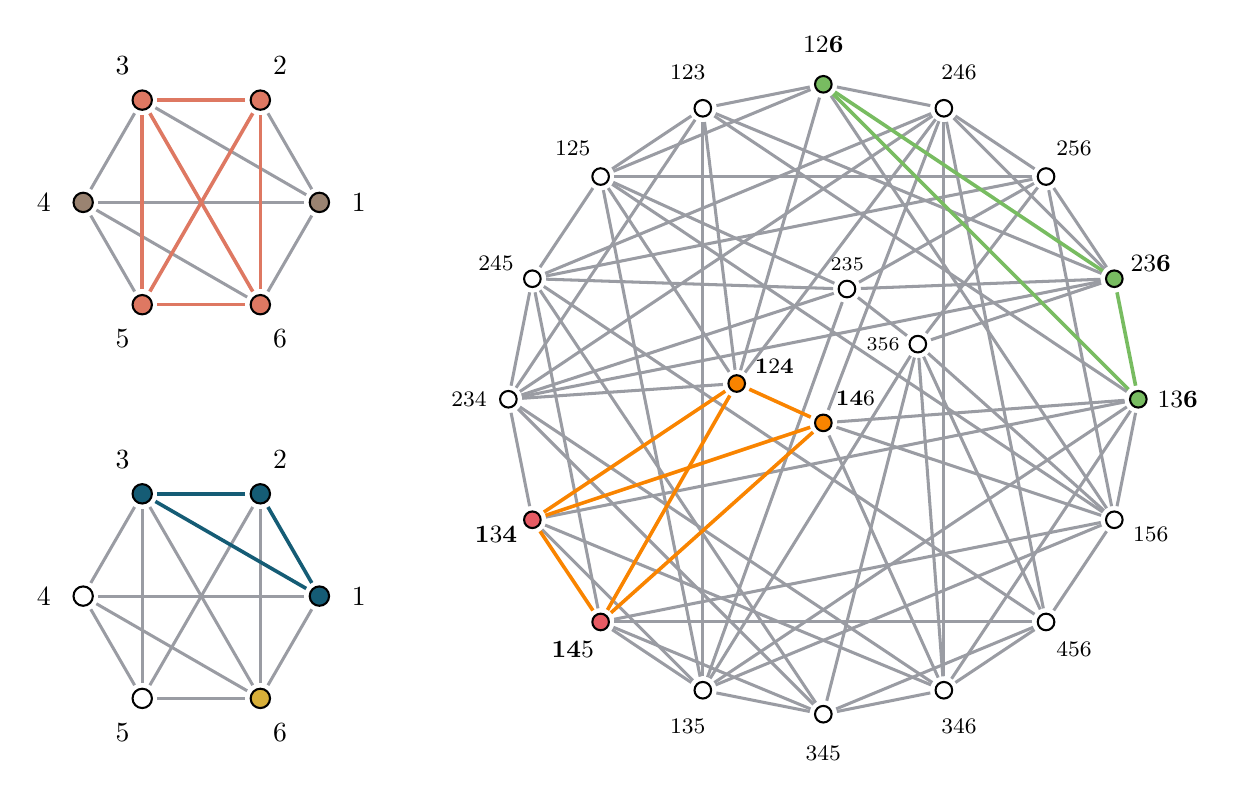
\begin{tikzpicture}
        
        \begin{scope}[xshift=-7.9cm,yshift=2.5cm]
                
            \foreach \i in {1,2,4,5}
                \draw ({(360/6)*\i}:1.5) node(\i)[bvertex,fill=salmon]{};
            \foreach \i in {0,3}
                \draw ({(360/6)*\i}:1.5) node(\i)[bvertex,fill=baige]{};
                    
            \foreach \i in {0,...,5}
                \draw ({(360/6)*\i}:2) node(e0){\pgfmathparse{int(\i+1)}
                \pgfmathresult};

            \foreach \i/\j in {0/1,0/2,0/3,0/5,2/3,3/4,3/5}
                \draw [edge,grisOscuro!60] (\i) to (\j);
                
            \foreach \i/\j in {1/2,4/5,1/5,2/4,2/5,1/4}
                \draw [wedge,salmon] (\i) to (\j);
        \end{scope}

        \begin{scope}[xshift=-7.9cm,yshift=-2.5cm]
                
            \foreach \i in {0,1,2}
                \draw ({(360/6)*\i}:1.5) node(\i)[bvertex,fill=azulOscuro]{};
            \foreach \i in {3,4}
                \draw ({(360/6)*\i}:1.5) node(\i)[bvertex]{};
        
                \draw ({(360/6)*5}:1.5) node(5)[bvertex,fill=oro]{};
                        
            \foreach \i in {0,...,5}
                \draw ({(360/6)*\i}:2) node(e0){\pgfmathparse{int(\i+1)}
                   \pgfmathresult};
    
            \foreach \i/\j in {0/3,0/5,1/4,1/5,2/3,2/4,2/5,3/4,3/5,4/5}
                \draw [edge,grisOscuro!60] (\i) to (\j);
                
                \foreach \i/\j in {0/1,0/2,1/2}
                \draw [wedge,azulOscuro] (\i) to (\j);
        \end{scope}
            
        \begin{scope}[xshift=0cm,yshift=0cm,scale=1]
            \foreach \i in {9,10} \draw ({(360/16)*\i}:4)
                node(\i)[wvertex,fill=rosa]{};
                
            \foreach \i in {0,1,4} \draw ({(360/16)*\i}:4)
                node(\i)[wvertex,fill=verde]{};
                
            \foreach \i in {2,3,5,6,7,8,11,12,13,14,15} \draw ({(360/16)*\i}:4)
                node(\i)[wvertex]{};
        
            \draw ({(360/16)*1}:4.5) node (e1) {{\small $23{\bf 6}$}};
            \draw ({(360/16)*2}:4.5) node (e1) {{\footnotesize $256$}};
            \draw ({(360/16)*3}:4.5) node (e1) {{\footnotesize $246$}};
            \draw ({(360/16)*4}:4.5) node (e1) {{\small $12{\bf 6}$}};
            \draw ({(360/16)*5}:4.5) node (e1) {{\footnotesize $123$}};
            \draw ({(360/16)*6}:4.5) node (e1) {{\footnotesize $125$}};
            \draw ({(360/16)*7}:4.5) node (e1) {{\footnotesize $245$}};
            \draw ({(360/16)*8}:4.5) node (e1) {{\footnotesize $234$}};
            \draw ({(360/16)*9}:4.5) node (e1) {{\small ${\bf 1}3{\bf 4}$}};
            \draw ({(360/16)*10}:4.5) node (e1) {{\small ${\bf 14}5$}};
            \draw ({(360/16)*11}:4.5) node (e1) {{\footnotesize $135$}};
            \draw ({(360/16)*12}:4.5) node (e1) {{\footnotesize $345$}};
            \draw ({(360/16)*13}:4.5) node (e1) {{\footnotesize $346$}};
            \draw ({(360/16)*14}:4.5) node (e1) {{\footnotesize $456$}};
            \draw ({(360/16)*15}:4.5) node (e1) {{\footnotesize $156$}};
            \draw ({(360/16)*16}:4.5) node (e1) {{\small $13{\bf 6}$}};
        
            \draw (-1.1,0.2) node (17) [vertex, fill=naranja, label=5:{\footnotesize ${\bf1}2{\bf 4}$}] {};
            \draw (0,-0.3) node (18) [vertex, fill=naranja, label=70:{\footnotesize ${\bf 14}6$}] {};
            \draw (1.2,0.7) node (19) [vertex, label=180:{\scriptsize $356$}] {};
            \draw (0.3,1.4) node (20) [vertex, label=88:{\scriptsize $235$}] {};
                
            \foreach\i/\j in{1/2,2/3,3/4,4/5,5/6,6/7,7/8,8/9,10/11,11/12,12/13,
                13/14, 14/15, 15/0} 
                \draw [edge,grisOscuro!60] (\i) to (\j);
                
            \foreach\i/\j in{0/5,0/11,0/13,1/3,1/5,2/6,2/7,2/15,3/7,3/8,4/6,
                4/15,5/8,6/11,6/15,7/10,7/12,8/12,8/13,9/11,9/13,10/12,10/14,
                10/15,11/15,12/14} 
                \draw [edge,grisOscuro!60] (\i) to (\j);
                
            \foreach \i/\j in{1/8,3/13,3/14,5/11,7/14,9/0,17/3,17/4,17/5,17/6,
                17/8,3/18,15/18,18/13,18/0,19/1,19/2,19/11,19/12,
                19/13,19/14,19/15,19/20,20/1,20/2,20/6,20/7,20/8,20/11}
                \draw [edge,grisOscuro!60] (\i) to (\j);
        

            \foreach\i/\j in{9/10,9/17,9/18,10/17,10/18,17/18} 
                \draw [wedge,naranja] (\i) to (\j);
                
            \foreach\i/\j in{0/1,0/4,1/4} 
                \draw [wedge,verde] (\i) to (\j);
        \end{scope}
        
    \end{tikzpicture}
\caption{Del lado izquierdo, dos copias de $G$, resaltando
${\color{salmon}\boldsymbol {K_1}}$ y ${\color{baige}\boldsymbol {S_1}}$ (copia
superior) y resaltando ${\color{azulOscuro}\boldsymbol {K_2}}$ y
${\color{oro}\boldsymbol {S_2}}$ (copia inferior). Del lado derecho, $F_3(G)$,
resaltando ${\color{naranja}\boldsymbol {X_1}}$ y ${\color{verde}\boldsymbol
{X_2}}$.}
\label{fig:ex-clique2}
\end{figure}
       
Por la caracterizaci\'on obtenida en \cref{teo:clanG-clanFG}, sabemos que un
clan $X$ en $F_k(G)$ tiene la misma cardinalidad que $K$, clan en $G$ como en el
teorema. Por ello, podr\'ia parecer que $G$ y $F_k(G)$ tienen el mismo n\'umero
de clan. Sin embargo, \cref{fig:ex-wG} nos muestra un ejemplo en el que el
n\'umero de clan de $G$ es mayor al de $F_k(G)$.


\begin{figure}[ht!]
    \centering
    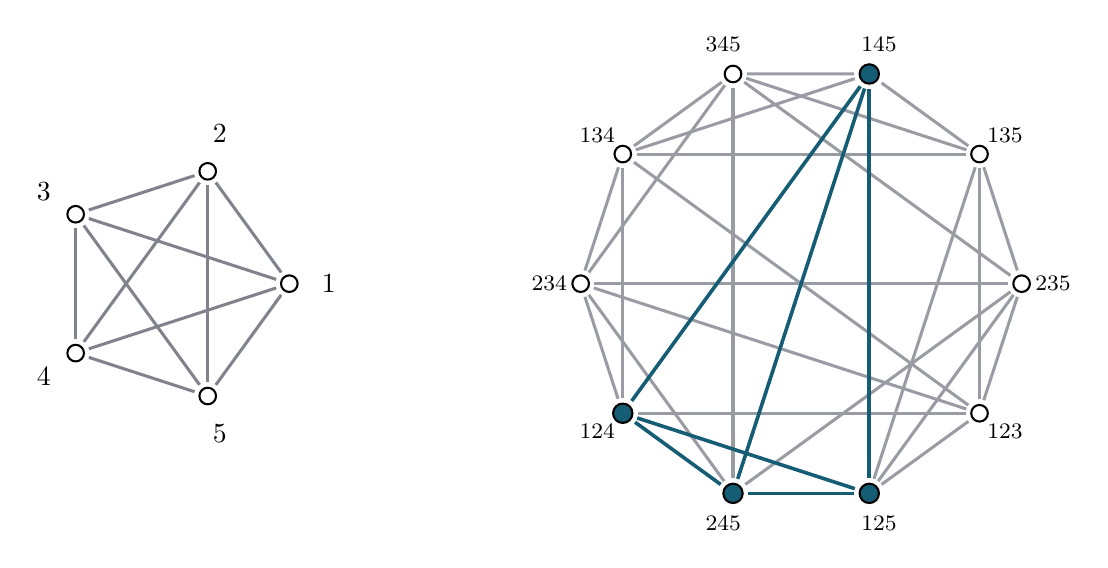
\begin{tikzpicture}

        \begin{scope}[xshift=-4cm]
                
            \foreach \i in {1,...,5}
                \draw ({(360/5)*\i}:1.5) node(\i)[vertex]{};
                        
            \foreach \i in {0,...,4}
                \draw ({(360/5)*\i}:2) node(e0){\pgfmathparse{int(\i+1)}
                   \pgfmathresult};
    
            \foreach \i/\j in {1/2,1/3,1/4,1/5,2/3,2/4,2/5,3/4,3/5,4/5}
                \draw [edge,grisOscuro!75] (\i) to (\j);
                
        \end{scope}
            
        \begin{scope}[xshift=4cm,yshift=0cm,scale=0.8]
            \foreach \i in {0,1,3,4,5,9} 
            \draw ({(360/10)*\i}:3.5) node(\i)[wvertex]{};

            \foreach \i in {2,6,7,8}
                \draw ({(360/10)*\i}:3.5) node(\i)[bvertex,fill=azulOscuro]{};
                
            \draw ({(360/10)*1}:4) node (e1) {{\footnotesize $135$}};
            \draw ({(360/10)*2}:4) node (e1) {{\footnotesize $145$}};
            \draw ({(360/10)*3}:4) node (e1) {{\footnotesize $345$}};
            \draw ({(360/10)*4}:4) node (e1) {{\footnotesize $134$}};
            \draw ({(360/10)*5}:4) node (e1) {{\footnotesize $234$}};
            \draw ({(360/10)*6}:4) node (e1) {{\footnotesize $124$}};
            \draw ({(360/10)*7}:4) node (e1) {{\footnotesize $245$}};
            \draw ({(360/10)*8}:4) node (e1) {{\footnotesize $125$}};
            \draw ({(360/10)*9}:4) node (e1) {{\footnotesize $123$}};
            \draw ({(360/10)*10}:4) node (e1) {{\footnotesize $235$}};
            
            \foreach\i/\j in{0/1,0/3,0/5,0/7,0/8,0/9,1/2,1/3,1/4,1/8,1/9,2/3,2/4,
            3/4,3/5,3/7,4/5,4/6,4/9,5/6,5/7,5/9,6/9,8/9} 
                \draw [edge,grisOscuro!60] (\i) to (\j);

            \foreach \i/\j in {2/6,2/7,2/8,6/7,6/8,7/8}
                \draw [wedge,azulOscuro] (\i) to (\j);
                
        \end{scope}
        
    \end{tikzpicture}
\caption{La gr\'afica $K_5$ (izquierda) y su gr\'afica de $3$-fichas, resaltando
un ${\color{azulOscuro}\bf {clan}}$ de cardinalidad $\omega(F_3(K_5))$
(derecha).}
\label{fig:ex-wG}
\end{figure}

Pasamos a determinar el n\'umero de clan de $F_k(G)$ en el siguiente teorema,
que nos da una f\'ormula para $\omega(F_k(G))$.
            
\begin{teorema}
\label{teo:clan-max}
    Si $G$ una gr\'afica y $F_k(G)$ su gr\'afica de $k$-fichas, entonces
    \[
    \omega(F_k(G))= \min \{\omega(G), \max \{n-k+1,k+1\}\}.
    \]
\end{teorema}

\begin{proof}
    Sea $X$ un clan de $F_k(G)$ con $\omega(F_k(G))$ v\'ertices. Sabemos que $X$
    satisface alguno de los incisos d\cref{teo:clanG-clanFG}. Para esta
    demostraci\'on, consideramos a $K$ como en el teorema anterior.   Si $X =
    \{S \cup \{v\} \colon\ v \in K\}$ y $|S| = k-1$, notamos que $|X| = |K|$.
    Adem\'as, tenemos que $n \geq |S| + |K|$. Por lo tanto, tenemos que $n \geq
    |S| + |K| = k-1 + |X|$, es decir, $|X| \leq n-k+1$. Por otro lado, si 
    \linebreak
    $X = \{(S\cup K) \setminus \{v\} \colon\ v \in K \}$ y $|S| + |K| = k+1$,
    notamos que tenemos la misma cardinalidad que en caso anterior, i.~e., $|X|
    =|K|$. Por ello, obtenemos $|X| = |K| \leq |S| + |K| = k+1$. Por lo tanto,
    de los dos casos, obtenemos que $|X| \leq \max\{n-k+1, k+1\}$.
    Adicionalmente, tenemos que ambos casos cumplen $|X| = |K| \leq \omega(G)$.
    Por lo que $\omega(F_k(G)) = |X| \leq \min \{\omega(G), \max \{n-k+1,
    k+1\}\}$ y, de esta manera, tenemos la cota superior de la ecuaci\'on
    deseada.

    Tomemos ahora un clan $K$ de $G$ con $\omega(G)$ v\'ertices. Consideramos
    las siguientes construcciones de clanes de $F_k(G)$. Primero, sea $K'$ un
    subconjunto de $K$ con $\min\{\omega(G),n-k+1\}$ v\'ertices, entonces
    tenemos que $|V(G) \setminus K'| \geq k-1$. Luego, sea $S$ un subconjunto de
    $V(G) \setminus K'$ con exactamente $k-1$ v\'ertices. Obtenemos un clan de
    $F_k(G)$ de la forma $\{ S \cup \{v\} \colon\ v \in K'\}$. Este clan tiene
    $|K'|$ v\'ertices. Por lo tanto, tenemos que $\omega(F_k(G)) \geq \min
    \{\omega(G), n-k+1\}$. Ahora, tomamos el subconjunto $K'$ de $K$ con $\min
    \{ \omega(G), k+1\}$ v\'ertices. Como $n \geq k+1$, entonces existe un
    subconjunto $S$ de $V(G) \setminus K'$ con $(k+1)-|K'|$ v\'ertices. As\'i
    pues, tenemos un clan de $F_k(G)$ de la forma $\{ (S \cup K') \setminus
    \{v\} \colon\ v \in K'\}$ que tiene $|K'|$ v\'ertices. Por lo tanto, tenemos
    que $\omega(F_k(G)) \geq \min \{\omega(G), k+1\}$.

    De los casos anteriores, tenemos que $\omega(F_k(G)) \geq  \min \{\omega(G),
    \max \{n-k+1,k+1\}\}$. De esta manera, obtenemos la cota inferior deseada.
    Por lo tanto, tenemos que se cumple la igualdad, i.~e., $\omega(F_k(G))=
    \min \{\omega(G), \max \{n-k+1,k+1\}\}$.
\end{proof}

Este teorema se puede simplificar como se muestra en el siguiente corolario. La
demostraci\'on de este corolario no se encuentra en el art\'iculo
\cite{fabilaToken}, pues sale de manera directa, utilizando \cref{teo:clan-max}.
Sin embargo, para este trabajo se considera pertinente incluir la
demostraci\'on, por lo que a continuaci\'on presentamos una demostraci\'on del
corolario.

\begin{corolario}
\label{coro:numClan}
    Sean $G$ un agr\'afica y $F_k(G)$ su gr\'afica de $k$-fichas. Si $k \leq
    \frac{n}{2}$, entonces $\omega(F_k(G))= \min\{\omega(G), n-k+1\}$.
\end{corolario}

\begin{proof}
    D\cref{teo:clan-max} tenemos $\omega(F_k(G))= \min \{\omega(G), \max
    \{n-k+1,k+1\}\}$. Basta demostrar que $\max \{n-k+1, k+1\} = n-k+1$. En
    otras palabras, 
    \linebreak
    $n-k+1 \geq k+1$. Esto \'ultimo pasa si y s\'olo si $n \geq
    2k$. Por lo tanto, si $\frac{n}{2} \geq k$, se cumple la igualdad deseada.
\end{proof}

Recordando que $F_k(G) \cong F_{n-k}(G)$, la utilidad  d\cref{coro:numClan}
resulta evidente. 

\section{N\'umero cr\'omatico}%
\label{sec:num cromatico}

En esta secci\'on estudiaremos el n\'umero crom\'atico de una gr\'afica de
$k$-fichas, es decir, $\chi (F_k(G))$. A diferencia de la secci\'on anterior,
acotamos el n\'umero crom\'atico de $F_k(G)$ utilizando el n\'umero crom\'atico
de $G$. Comenzamos con la cota superior de $ \chi (F_k(G))$ en el siguiente
teorema, cuya demostraci\'on sale del art\'iculo \textit{Token graphs}
\cite{fabilaToken}.

\begin{teorema}
\label{teo:num cromatico de G y F(G)}
    Sea $G$ una gr\'afica y $F_k(G)$ su gr\'afica de $k$-fichas, entonces
    \[
        \chi(F_k(G)) \leq \chi (G).
    \]
\end{teorema}

\begin{proof}
    Sea $c \colon V(G) \to \{0,1, \dots, \chi(G)-1\}$ una coloraci\'on propia de
    $G$. Ahora, a cada v\'ertice $A$ de $F_k(G)$ le asignamos el color $ c'(A)=
    \Sigma_{x \in A}c(x)$ m\'odulo $\chi(G)$. Basta ver que $c'$ es una
    coloraci\'on propia. Suponemos lo contrario, que existen $A$ y $B$
    v\'ertices adyacentes en $F_k(G)$, tales que $c'(A) = c'(B)$. Como $A$ y $B$
    son adyacentes, entonces $A \triangle B = \{a,b\}$, para algunos v\'ertices
    $a$ y $b$ de $G$, tales que $ab \in E(G)$. Al ser $c'(A) = c'(B)$, tenemos
    que $\Sigma_{x \in A}c(x) \equiv \Sigma_{y \in B}c(y) \pmod {\chi(G)}$. Sin
    p\'erdida de generalidad, consideramos $a \in A$ y $b \in B$, entonces
    podemos ver la congruencia de la siguiente manera:
    \[ c(a) + \Sigma_{x \in A \setminus\{a\}}c(x) \equiv c(b) + \Sigma_{y \in
    B\setminus\{b\}}c(y) \mod \chi(G).
    \] 
    Pero $A \triangle B = \{a,b\}$, por lo
    que $\Sigma_{x \in A\setminus\{a\}}c(x)=\Sigma_{y \in B\setminus\{b\}}c(y)$,
    entonces tenemos que $c(a) \equiv c(b) \mod \chi(G)$. De este modo llegamos
    a la contradicci\'on de que $c$ no es una coloraci\'on propia, pues $c(a) =
    c(b)$ y $ab \in E(G)$. Por lo que tenemos que $c'$ es una coloraci\'on
    propia de $F_k(G)$ con, a lo m\'as, $\chi (G)$ colores. Por lo tanto,
    $\chi(F_k(G)) \leq \chi (G)$.
\end{proof}

Nos enfocamos ahora en la cota inferior de $ \chi (F_k(G))$. Sabemos que $\chi
(G) \geq \omega (G)$ para todas las gr\'aficas, por lo que podemos sacar una
cota inferior en t\'erminos de el n\'umero de clan de $G$, utilizando
\cref{teo:clan-max}. Por otro lado, podemos encontrar una cota en t\'erminos de
$\chi (G)$. \Cref{prop:biparticion F(G)} y \cref{teo:numCrom-k}, a
continuaci\'on exhibidos, tienen demostraci\'ones basadas en el art\'iculo
\textit{Token graphs} \cite{fabilaToken}. Empezamos viendo
\cref{prop:biparticion F(G)}, una propiedad sobre las gr\'aficas bipartitas en
gr\'aficas de fichas.

\begin{proposicion}
\label{prop:biparticion F(G)}
    Sea $F_k(G)$ una gr\'afica bipartita, para $k \geq 1$, entonces $F_l(G)$ es
    una gr\'afica bipartita para todo $l \geq 1$.
\end{proposicion}

\begin{proof}
    Para empezar, veamos que, si $F_k(G)$ es una gr\'afica bipartita, entonces
    $G$ es una gr\'afica bipartita. Lo probamos por contrapositiva, es decir, si
    $G$ no es una gr\'afica bipartita, entonces $F_k(G)$ tampoco es una
    gr\'afica bipartita. Sea $G$ una gr\'afica que no es bipartita, entonces $G$
    contiene un ciclo impar $C=(v_1, \dots, v_{p-1}, v_p, v_1)$. Primero, veamos
    el caso en el que $p \geq k+1$. En este caso $F_k(G)$ tiene un $p$-ciclo de
    la siguiente manera: 
    \[
    (\{v_1, v_2, \dots, v_{k-2}, v_{k-1},v_k\},\{v_1, v_2, \dots, v_{k-2}, v_{k-1}, v_{k+1}\},\]
    \[\{v_1, v_2, \dots, v_{k-2}, v_{k-1}, v_{k+2}\},\cdots,\{v_1, v_2, \dots, v_{k-2}, v_{k-1},v_p\},\]
    \[\{v_1, v_2, \dots, v_{k-2}, v_k, v_p\},\{v_1, v_2, \dots, v_{k-1},v_k, v_p\},
    \dots,\{v_1, v_3, \dots, v_{k-1}, v_k, v_p\},\]
    \[\{v_2, v_3,\dots, v_{k-1}, v_k, v_p\},\{v_1, v_2, \dots, v_{k-2}, v_{k-1}, v_k\})
    \]
    Notamos que, hay $p-k+1$ v\'ertices al mover la ficha de $v_k$ a $p$.
    Adem\'as, tenemos $k-1$ v\'ertices en el resto del ciclo. Por lo tanto,
    $F_k(G)$ tiene un $p$-ciclo, por lo que no es bipartita.
    
    Ahora, consideramos el caso en el que $p \leq k$. Notamos que, el conjunto
    $V(G)\setminus C$ tiene cardinalidad $n-p$, donde $C$ es el ciclo impar
    antes mencionado. Como $n \geq k+1$, entonces $n-p \geq k+1-p$, por lo que
    existe un conjunto $A$ de $k-p+1$ v\'ertices en $V(G)\setminus C$. Notemos
    que, al colocar una ficha en cada v\'ertice de $A$ y mantenerlas fijas, o
    equivalentemente s\'olo mover las $p-1$ fichas restantes, se obtiene una
    gr\'afica isomorfa a la gr\'afica de fichas $F_{p-1}(G-A)$. De este modo,
    tenemos el caso anterior, en el que $k \leq p$, que $F_{p-1}(G-A)$ no es una
    gr\'afica bipartita. Pero, como ya notamos, $F_{p-1}(G-A) = F_{k-(k+1-p)}
    (G-A)$ es isomorfa a la subgr\'afica de $F_k(G)$ inducida por los v\'ertices
    de $F_k(G)$ que contienen a $A$, $F_k(G,A)$. Por lo tanto, existe un ciclo
    impar en una gr\'afica inducida de $F_k(G)$, de manera que $F_k(G)$ no es
    bipartita. Por lo tanto, tenemos que si $F_k(G)$ es una gr\'afica bipartita,
    entonces $G$ tambi\'en lo es.

    Pasamos a demostrar la proposici\'on. Sea $F_k(G)$ una gr\'afica bipartita,
    por lo demostrado anteriormente, tenemos que $G$ tambi\'en es una gr\'afica
    bipartita. Sabemos que, una gr\'afica es $2$-crom\'atica si y s\'olo si es
    bipartita y no vac\'ia, por lo que $\chi(G)=2$. Pero, por \cref{teo:num
    cromatico de G y F(G)}, tenemos para cualquier $l\geq 1$, $\chi (F_l(G)) \le
    \chi (G) = 2$. Por lo tanto, tenemos que $F_l(G)$ es $2$-crom\'atica, i.~e.,
    es una gr\'afica bipartita.
\end{proof}

\begin{figure}[ht!]
    \centering
    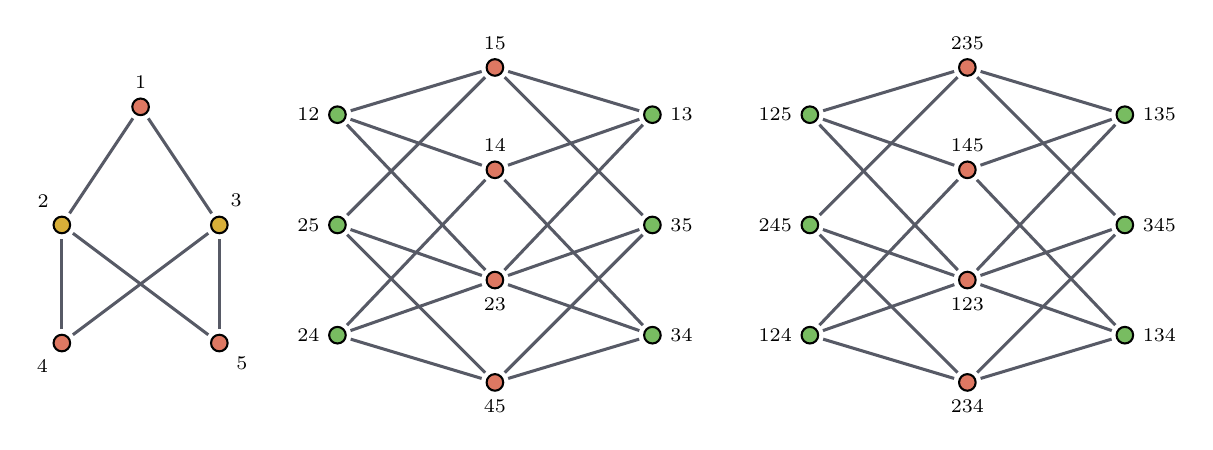
\begin{tikzpicture}
    
        \begin{scope}[xshift=-5.5cm]
            \draw (0,1.5) node (1) [vertex,fill=salmon ,label=90:{\scriptsize $1$}] {};
            \draw (-1,0) node (2) [vertex,fill=oro ,label=115:{\scriptsize $2$}] {};
            \draw (1,0) node (3) [vertex,fill=oro ,label=80:{\scriptsize $3$}] {};
            \draw (-1,-1.5) node (4) [vertex,fill=salmon ,label=240:{\scriptsize $4$}] {};
            \draw (1,-1.5) node (5) [vertex,fill=salmon ,label=330:{\scriptsize $5$}] {};

            \foreach \i/\j in{1/2,1/3,4/2,4/3,5/2,5/3} 
                \draw [edge,grisOscuro] (\i) to (\j);
        \end{scope}
        
        \begin{scope}[xshift=-1cm,yshift=0cm,scale=1]
            \draw (-2,1.4) node (1) [vertex,fill=verde ,label=180:{\scriptsize $12$}] {};
            \draw (2,1.4) node (2) [vertex,fill=verde ,label=0:{\scriptsize $13$}] {};
            \draw (0,0.7) node (3) [vertex,fill=salmon ,label=90:{\scriptsize $14$}] {}; 
            \draw (0,2) node (4) [vertex,fill=salmon ,label=90:{\scriptsize $15$}] {};
            \draw (0,-0.7) node (5) [vertex,fill=salmon ,label=270:{\scriptsize $23$}] {};
            \draw (-2,-1.4) node (6) [vertex,fill=verde ,label=180:{\scriptsize $24$}] {};
            \draw (-2,0) node (7) [vertex,fill=verde ,label=180:{\scriptsize $25$}] {};
            \draw (2,-1.4) node (8) [vertex,fill=verde ,label=0:{\scriptsize $34$}] {};
            \draw (2,0) node (9) [vertex,fill=verde ,label=0:{\scriptsize $35$}] {};
            \draw (0,-2) node (10) [vertex,fill=salmon ,label=270:{\scriptsize $45$}] {};
           
            \foreach \i/\j in{1/5,1/3,1/4,6/5,6/3,6/10,7/5,7/4,7/10,5/2,5/8,5/9,
                2/3,2/4,8/3,8/10,9/4,9/10} 
                \draw [edge,grisOscuro] (\i) to (\j);
       \end{scope}
    
       \begin{scope}[xshift=5cm,yshift=0cm,scale=1]
            \draw (0,-0.7) node (1) [vertex,fill=salmon ,label=270:{\scriptsize $123$}] {};
            \draw (-2,-1.4) node (2) [vertex,fill=verde ,label=180:{\scriptsize $124$}] {};
            \draw (-2,1.4) node (3) [vertex,fill=verde ,label=180:{\scriptsize $125$}] {};
            \draw (2,-1.4) node (4) [vertex,fill=verde ,label=0:{\scriptsize $134$}] {};
            \draw (2,1.4) node (5) [vertex,fill=verde ,label=0:{\scriptsize $135$}] {};
            \draw (0,0.7) node (6) [vertex,fill=salmon ,label=90:{\scriptsize $145$}] {}; 
            \draw (0,-2) node (7) [vertex,fill=salmon ,label=270:{\scriptsize $234$}] {};
            \draw (0,2) node (8) [vertex,fill=salmon ,label=90:{\scriptsize $235$}] {};
            \draw (-2,0) node (9) [vertex,fill=verde ,label=180:{\scriptsize $245$}] {};
            \draw (2,0) node (10) [vertex,fill=verde ,label=0:{\scriptsize $345$}] {};
            
            \foreach \i/\j in{5/1,5/6,5/8,2/1,2/6,2/7,10/1,10/8,10/7,1/3,1/4,1/9,
                3/6,3/8,4/6,4/7,9/8,9/7} 
                \draw [edge,grisOscuro] (\i) to (\j);
        \end{scope}
            
    
    \end{tikzpicture}
\caption{Una gr\'afica bipartita, su gr\'afica de $2$-fichas y su gr\'afica de
 $3$-fichas.}
\label{fig:ex-bip}
\end{figure}


\Cref{fig:ex-bip}, mostrada arriba, brinda un ejemplo de \cref{prop:biparticion
F(G)}, donde, de izquierda a derecha, se muestra una gr\'afica bipartita $G$, su
gr\'afica de $2$ y $3$-fichas. Notamos que, dada la bipartici\'on
$({\color{oro}\boldsymbol {X}},{\color{salmon}\boldsymbol {Y}})$ de $G$, toda
$F_l(G)$ con $l\geq 2$, tiene la bipartici\'on $({\color{verde} \boldsymbol
{Z}},{\color{salmon}\boldsymbol {W}})$, donde ${\color{verde}\boldsymbol
{Z=\{V\in X\colon\ (\{2\}\subseteq V  \lor \{3\} \subseteq V) \land
\{2,3\}\not\subseteq V\}}}$ y ${\color{salmon}\boldsymbol {W=\{V \in Y\colon\
\{2,3\}\subseteq V \lor \{2,3\}\not\subseteq V\}}}$. En otras palabras, para
toda gr\'afica de fichas de $G$, el conjunto ${\color{verde}\boldsymbol {Z}}$ es
el conjunto que contiene a ${\color{oro}\boldsymbol {X}}\in G$, o no lo
contiene. Adem\'as, el conjunto ${\color{salmon}\boldsymbol {W}}$ es el conjunto
que tiene exactamente un elemento de ${\color{oro}\boldsymbol {X}}\in G$.

Por \'ultimo, determinamos la cota inferior para $\chi (F_k(G))$ en t\'erminos
de $\chi (G)$ para el caso general.

\begin{teorema}
\label{teo:numCrom-k}
    Sea $G$ una gr\'afica. Si $F_k(G)$ es la gr\'afica de $k$-fichas de $G$,
    entonces
    \[
        \chi(F_k(G)) \geq \frac{n-k+2}{n} \chi(G) -1.
    \]
\end{teorema}

\begin{proof}
    Primero consideramos $k=1$. Sabemos que $n \geq \chi(G)$, por lo que tenemos
    que $n\chi(G) \geq n\chi(G) + \chi(G) -n$. As\'i pues, $\chi (G) \geq
    \frac{(n+1)\chi(G)-n}{n} = \frac{n+1}{n}\chi (G) -1$. Por otra parte,
    $F_1(G) \cong (G)$. Por lo tanto, tenemos que $\chi(F_1(G)) \geq
    \frac{n-1+2}{n} \chi(G) -1$.
        
    En segundo lugar, suponemos $k \geq 2$ y consideramos una coloraci\'on de
    $\chi(G)$ colores en $G$. Nombramos $V_1, V_2, \dots, V_{\chi(G)}$ a las
    clases crom\'aticas de $G$. Sin p\'erdida de generalidad, consideramos que
    $|V_1|\geq |V_2|\geq \cdots \geq |V_{\chi(G)}|$. Al tomar este orden, todo
    \'indice $m$ cumple que $\Sigma_{i=1}^{m}|V_i| \geq \frac{mn}{\chi(G)}$, con
    la igualdad en el caso en el que $|V_i| = |V_j| = \frac{n}{\chi(G)}$, para
    todo $i,j \in \{1, \dots, \chi(G)\}$. Denotamos con $m'$ el menor \'indice,
    tal que $\Sigma_{i=1}^{m'}|V_i| \geq k-1$. Notamos que
    $\Sigma_{i=1}^{m'-1}|V_i| \leq k-2$, pues de lo contrario tendr\'iamos que
    $k-2<\Sigma_{i=1}^{m'-1}|V_i| < k-1$, es decir, $\Sigma_{i=1}^{m'-1}|V_i|
    \notin \mathbb{Z}$. Luego, tenemos que $\frac{(m'-1)n}{\chi(G)}\leq
    \Sigma_{i=1}^{m'-1}|V_i| \leq k-2$. Ahora, tomamos $X \subseteq
    \bigcup_{i=1}^{m'} V_i$ con cardinalidad $k-1$. Por como se defini\'o el
    conjunto, $G[X]$ es $m'$-coloreable. Sabemos que, para un conjunto $S
    \subset V(G)$, se cumple que $\chi(G) \leq \chi(G[S])+\chi(G-S)$. Por lo que
    tenemos que $\chi(G) \leq \chi(G[X])+\chi(G-X) \leq m' + \chi(G-X)$.

    Ahora, sabemos que $F_{k-r}(G-H) \cong F_k(G,H)$, donde $r = |X|$. En este
    caso, $|X| = k-1$, as\'i tenemos que $F_1(G-X) \cong F_k(G,X)$. Adem\'as,
    sabemos que $F_1(G) \cong G$. Lo que implica que $G-X \cong F_k(G,X)$, que
    es una subr\'afica de $F_k(G)$. Por lo tanto, $\chi(G) \leq m' + \chi(G-X) =
    m' + \chi(F_k(G,X)) \leq m' + \chi(F_k(G))$. 
            
    Por otro lado, tenemos $\frac{(m'-1)n}{\chi(G)}\leq \Sigma_{i=1}^{m'-1}|V_i|
    \leq k-2$. As\'i, $m'-1 \leq \frac{(k-2)}{n}\chi(G)$, de donde se sigue que
    $\chi(G) \leq m' + \chi(F_k(G)) = \frac{(k-2)}{n}\chi(G) +1 + \chi(F_k(G))$.
    Por lo tanto, $\chi(F_k(G)) \geq \frac{n-k+2}{n} \chi(G) -1$
\end{proof}

A partir d\cref{teo:numCrom-k} podemos encontrar una cota inferior para
$\chi(F_k(G))$ que sea independiente de $k$. Esta relaci\'on se demuestra en el
siguiente teorema, cuya demostraci\'on no se desarrolla en el art\'iculo
\textit{Token graphs} \cite{fabilaToken}, de donde sale el teorema.


\begin{teorema}
\label{teo:numCrom indep-k}
    Si $G$ es una gr\'afica y $F_k(G)$ su gr\'afica de $k$-fichas, entonces
    \linebreak
    $\chi (F_k(G)) \geq (\frac{1}{2}+ \frac{2}{n})\chi(G) -1 $, para toda $k
    \geq 1$.
\end{teorema}
    
\begin{proof}
    Sea $G$ una gr\'afica y $F_k(G)$ su gr\'afica de fichas, con $k \geq 1$.
    D\cref{teo:numCrom-k}, tenemos que $\chi(F_k(G)) \geq \frac{n-k+2}{n}
    \chi(G) -1$. Basta demostrar que $\frac{n-k+2}{n} \geq
    \frac{1}{2}+\frac{2}{n}$. Sabemos que $F_k(G) \cong F_{n-k}(G)$, por lo que
    podemos asumir, sin p\'erdida de generalidad, que $k\leq \frac{n}{2}$.
    Luego, tenemos que $\frac{2n-n}{2}\geq k$, de donde obtenemos que $n-k \geq
    \frac{n}{2}$, entonces tenemos que $\frac{n-k}{n}\geq \frac{1}{2}$. Por lo
    tanto, $\frac{n-k+2}{n} \geq \frac{1}{2}+\frac{2}{n}$.
\end{proof}
\chapter{N\'umero Cr\'omatico}%
\label{cap:num cromatico}

\section{Teoremas y demostraciones}%
%\label{sec:etiquetas}


\begin{teorema}
\label{teo:num cromatico de G y F(G)}
    Sea $G$ una gr\'afica y $F_k(G)$ su $k$-gr\'afica de fichas, entonces
    $\chi(F_k(G)) \leq \chi (G)$.
\end{teorema}

\begin{proof}
    Sea $c: V(G) \to \{0,1, \dots, \chi(G)-1\}$ una coloraci\'on propia de $G$.
    Ahora, a cada v\'ertice $A$ de $F_k(G)$ le asignamos el color $ c'(A)=
    \Sigma_{x \in A}c(x) \mod \chi(G)$. Basta ver que $c'$ es una coloraci\'on
    propia. Supongamos lo contrario, existen $A$ y $B$ v\'ertices adyacentes en
    $F_k(G)$ tales que $c'(A) = c'(B)$. Como $A$ y $B$ son adyacentes, entonces
    $A \triangle B = \{a,b\}$ para algunos v\'ertices $a$ y $b$ de $G$ tales que
    $ab \in E(G)$. Al tomar $c'(A) = c'(B)$ tenemos que $\Sigma_{x \in A}c(x)
    \equiv \Sigma_{y \in B}c(y) \mod \chi(G)$. Sin p\'erdida de generalidad
    consideramos $a \in A$ y $b \in B$, entonces podemos ver la congruencia de
    la siguiente manera: $c(a) + \Sigma_{x \in A \setminus\{a\}}c(x) \equiv c(b)
    + \Sigma_{y \in B\setminus\{b\}}c(y) \mod \chi(G)$. Pero $A \triangle B =
    \{a,b\}$, por lo que $\Sigma_{x \in A\setminus\{a\}}c(x)=\Sigma_{y \in
    B\setminus\{b\}}c(y)$. Entonces tenemos que $c(a) \equiv c(b) \mod \chi(G)$
    y de este modo llegamos a la contradicci\'on de que $c$ no es una
    coloraci\'on propia pues $c(a) = c(b)$ y $ab \in E(G)$. Por lo que tenemos
    que $c'$ es una coloraci\'on propia de $F_k(G)$ con a lo m\'as $\chi (G)$
    colores. Por lo tanto $\chi(F_k(G)) \leq \chi (G)$.
\end{proof}

\begin{proposicion}
\label{prop:biparticion F(G)}
    Sea $F_k(G)$ una gr\'afica bipartita para $k \geq 1$, entonces $F_l(G)$
    es una gr\'afica bipartita para todo $l \geq 1$.
\end{proposicion}

%demostrar en el cap de gr\'aficas que una gráfica es 1-cromática si y sólo
%si es vacı́a, y es 2-cromática si
%y sólo si es bipartita y no vacı́a
\begin{proof}
    Para empezar, veamos que si $F_k(G)$ es una gr\'afica bipartita, entonces
    $G$ es una gr\'afica bipartita. Lo probaremos por contrapositiva, es decir,
    si $G$ no es una gr\'afica bipartita, entonces $F_k(G)$ tampoco es una
    gr\'afica bipartita. Sea $G$ una gr\'afica que no es bipartita, entonces $G$
    contiene un ciclo impar $C=(v_1, \dots, v_{p-1}, v_p, v_1)$. Primero veamos
    el caso en el que $p \geq k+1$. En este caso tenemos un $p$-ciclo en
    $F_k(G)$ de la siguiente manera: $\{v_1, v_2, \dots, v_{k-2}, v_{k-1},
    v_k\}$ $\{v_1, v_2, \dots, v_{k-2}, v_{k-1}, v_{k+1}\}$ $\{v_1, v_2, \dots,
    v_{k-2}, v_{k-1}, v_{k+2}\}, \dots, \{v_1, v_2, \dots, v_{k-2}, v_{k-1},
    v_p\}$ $\{v_1, v_2, \dots, v_{k-2}, v_k, v_p\}$ $\{v_1, v_2, \dots, v_{k-1},
    v_k, v_p\} \dots \{v_1, v_3, \dots, v_{k-1}, v_k, v_p\}$ $\{v_2, v_3,
    \dots, v_{k-1}, v_k, v_p\}$ $\{v_1, v_2, \dots, v_{k-2}, v_{k-1}, v_k\}$.
    Notamos que el hay $p-k+1$ v\'ertices al mover la ficha de $v_k$ a $p$.
    Adem\'as tenemos $k-1$ v\'ertices en el resto del ciclo. Por lo tanto
    $F_k(G)$ tiene un $p$-ciclo por lo que no es bipartita.
    
    Ahora consideramos el caso en el que $p \leq k$. Notamos que el conjunto
    $V(G)\setminus C$ tiene cardinalidad $n-p$, donde $C$ es el ciclo impar
    antes mencionado. Como $n \geq k+1$, entonces $n-p \geq k+1-p$, por lo que
    existe un conjunto $A$ de $k-p+1$ v\'ertices en $V(G)\setminus C$. Notemos
    que al colocar una ficha en cada v\'ertice de $A$, y mantenerlas fijas, o
    equivalentemente s\'olo mover las $p-1$ fichas restantes, se obtiene una
    gr\'afica isomorfa a la gr\'afica de fichas $F_{p-1}(G-A)$. Entonces tenemos
    del caso anterior, en el que $k \leq p$, que $F_{p-1}(G-A)$ no es una
    gr\'afica bipartita. Pero como ya notamos, $F_{p-1}(G-A) = F_{k-(k+1-p)}
    (G-A)$ es isomorfa a la subgr\'afica de $F_k(G)$ inducida por los v\'ertices
    de $F_k(G)$ que contienen a $A$, $F_k(G,A)$. Por lo tanto existe un ciclo
    impar en una gr\'afica inducida de $F_k(G)$, de manera que $F_k(G)$ no es
    bipartita. Por lo tanto tenemos que si $F_k(G)$ es una gr\'afica bipartita,
    entonces $G$ tambi\'en lo es.

    Ahora pasamos a demostrar la proposici\'on. Sea $F_k(G)$ una gr\'afica
    bipartita, por lo demostrado anteriormente, tenemos que $G$ tambi\'en es una
    gr\'afica bipartita. Sabemos que una gr\'afica es $2$-crom\'atica si y
    s\'olo si es bipartita y no vac\'ia, por lo que $\chi(G)=2$. Pero, por
    \cref{teo:num cromatico de G y F(G)}, tenemos para cualquier $l\geq 1$,
    $\chi (F_l(G)) \le \chi (G) = 2$. Por lo tanto tenemos que $F_l(G)$ es
    $2$-crom\'atica, es decir es una gr\'afica bipartita.
\end{proof}



\begin{figure}[ht!]
    \centering
       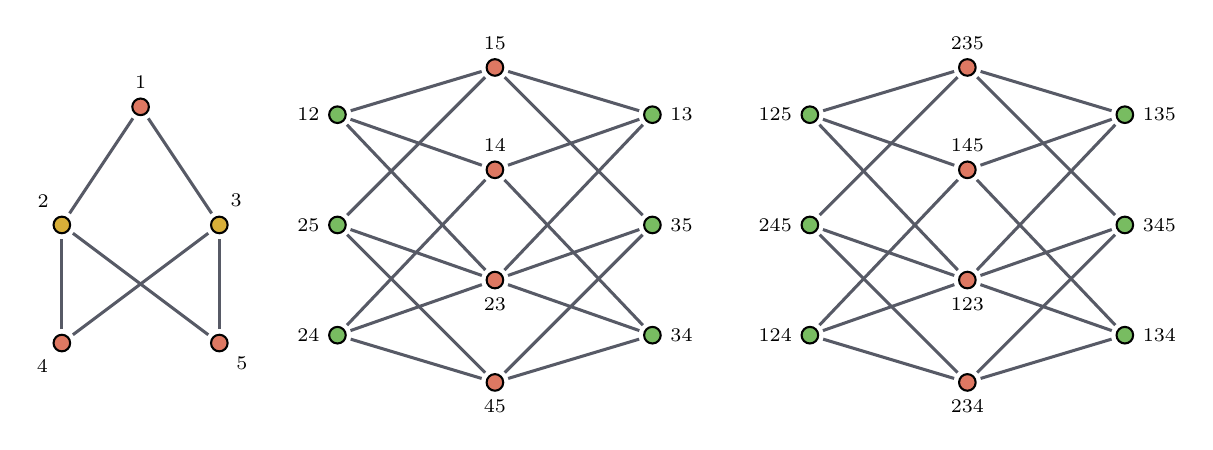
\begin{tikzpicture}
    
        \begin{scope}[xshift=-5.5cm]
            \draw (0,1.5) node (1) [vertex,fill=salmon ,label=90:{\scriptsize $1$}] {};
            \draw (-1,0) node (2) [vertex,fill=amarilloOscuro ,label=115:{\scriptsize $2$}] {};
            \draw (1,0) node (3) [vertex,fill=amarilloOscuro ,label=80:{\scriptsize $3$}] {};
            \draw (-1,-1.5) node (4) [vertex,fill=salmon ,label=240:{\scriptsize $4$}] {};
            \draw (1,-1.5) node (5) [vertex,fill=salmon ,label=330:{\scriptsize $5$}] {};

            \foreach \i/\j in{1/2,1/3,4/2,4/3,5/2,5/3} 
            \draw [edge,grisOscuro] (\i) to (\j);
            \end{scope}
        
        \begin{scope}[xshift=-1cm,yshift=0cm,scale=1]
            \draw (-2,1.4) node (1) [vertex,fill=verde ,label=180:{\scriptsize $12$}] {};
            \draw (2,1.4) node (2) [vertex,fill=verde ,label=0:{\scriptsize $13$}] {};
            \draw (0,0.7) node (3) [vertex,fill=salmon ,label=90:{\scriptsize $14$}] {}; 
            \draw (0,2) node (4) [vertex,fill=salmon ,label=90:{\scriptsize $15$}] {};
            \draw (0,-0.7) node (5) [vertex,fill=salmon ,label=270:{\scriptsize $23$}] {};
            \draw (-2,-1.4) node (6) [vertex,fill=verde ,label=180:{\scriptsize $24$}] {};
            \draw (-2,0) node (7) [vertex,fill=verde ,label=180:{\scriptsize $25$}] {};
            \draw (2,-1.4) node (8) [vertex,fill=verde ,label=0:{\scriptsize $34$}] {};
            \draw (2,0) node (9) [vertex,fill=verde ,label=0:{\scriptsize $35$}] {};
            \draw (0,-2) node (10) [vertex,fill=salmon ,label=270:{\scriptsize $45$}] {};
           
            \foreach \i/\j in{1/5,1/3,1/4,6/5,6/3,6/10,7/5,7/4,7/10,5/2,5/8,5/9,
            2/3,2/4,8/3,8/10,9/4,9/10} 
            \draw [edge,grisOscuro] (\i) to (\j);
       \end{scope}
    
       \begin{scope}[xshift=5cm,yshift=0cm,scale=1]
            \draw (0,-0.7) node (1) [vertex,fill=salmon ,label=270:{\scriptsize $123$}] {};
            \draw (-2,-1.4) node (2) [vertex,fill=verde ,label=180:{\scriptsize $124$}] {};
            \draw (-2,1.4) node (3) [vertex,fill=verde ,label=180:{\scriptsize $125$}] {};
            \draw (2,-1.4) node (4) [vertex,fill=verde ,label=0:{\scriptsize $134$}] {};
            \draw (2,1.4) node (5) [vertex,fill=verde ,label=0:{\scriptsize $135$}] {};
            \draw (0,0.7) node (6) [vertex,fill=salmon ,label=90:{\scriptsize $145$}] {}; 
            \draw (0,-2) node (7) [vertex,fill=salmon ,label=270:{\scriptsize $234$}] {};
            \draw (0,2) node (8) [vertex,fill=salmon ,label=90:{\scriptsize $235$}] {};
            \draw (-2,0) node (9) [vertex,fill=verde ,label=180:{\scriptsize $245$}] {};
            \draw (2,0) node (10) [vertex,fill=verde ,label=0:{\scriptsize $345$}] {};
            
        \foreach \i/\j in{5/1,5/6,5/8,2/1,2/6,2/7,10/1,10/8,10/7,1/3,1/4,1/9,
            3/6,3/8,4/6,4/7,9/8,9/7} 
            \draw [edge,grisOscuro] (\i) to (\j);
   \end{scope}
            
    
    \end{tikzpicture}
    \caption{Gr\'afica bipartita, su 2-gr\'afica de fichas y su 3-gr\'afica de fichas.}
    \label{fig:ex-bip}
\end{figure}

Notamos que, dada la bipartici\'on
$({\color{amarilloOscuro}X},{\color{salmon}Y})$, toda $F_l(G)$, con $l\geq 2$,
tiene la bipartici\'on $({\color{verde}X},{\color{salmon}Y})$, donde
${\color{verde}X=\{V\in X\colon\ (\{2\}\subseteq V  \lor \{3\} \subseteq V)
\land \{2,3\}\not\subseteq V\}}$ y 

${\color{salmon}Y=\{V \in Y\colon\ \{2,3\}\subseteq V \lor \{2,3\}\not\subseteq
V\}}$. En otras palabras, para toda gr\'afica de fichas de $G$,el conjunto
${\color{verde}X}$ es el conjunto que contiene a
${\color{amarilloOscuro}X}\in G$ o no lo contiene. Adem\'as, el conjunto
${\color{salmon}Y}$ es el conjunto que tiene exactamente un elemente de
${\color{amarilloOscuro}X}\in G$    

    \begin{teorema}
        \label{relacion num cromatico G y F(G) con k}
            Sea $G$ una gr\'afica y $F_k(G)$ su $k$-gr\'afica de fichas.
            Entonces $\chi(F_k(G)) \geq \frac{n-k+2}{n} \chi(G) -1$.
        \end{teorema}
        
        %definici\ón de grafica inducida dem n\'umero crom\'atico de
        %subgr\'afica menor a n\'umero cr\'omatioc de gr\'afica 
        \begin{proof}
        Primero consideramos $k=1$. Sabemos que $n \geq \chi(G)$, por lo que
        tenemos que $n\chi(G) \geq n\chi(G) + \chi(G) -n$. Entonces obtenemos
        $\chi (G) \geq \frac{(n+1)\chi(G)-n}{n} = \frac{n+1}{n}\chi (G) -1$.
        Por otra parte, $F_1(G) \cong (G)$. Por lo tanto tenemos que
        $\chi(F_1(G)) \geq \frac{n-1+2}{n} \chi(G) -1$.
        
            Ahora supongamos $k \geq 2$ y una coloraci\'on de $\chi(G)$ colores
            en $G$. Nombramos $V_1 V_2, \dots, V_{\chi(G)}$ a las clases
            crom\'aticas de $G$. Sin p\'erdida de generalidad, consideramos que
            $|V_1|\geq |V_2|\geq \cdots \geq |V_{\chi(G)}|$. Al tomar este
            orden, todo \'indice $m$ cumple que $\Sigma_{i=1}^{m}|V_i| \geq
            \frac{mn}{\chi(G)}$, con la igualdad en el caso en el que $|V_i| =
            |V_j| = \frac{n}{\chi(G)}$, para todo $i,j \in \{1, \dots,
            \chi(G)\}$. Denotamos con $m'$ el menor \'indice tal que
            $\Sigma_{i=1}^{m'}|V_i| \geq k-1$. Notamos que
            $\Sigma_{i=1}^{m'-1}|V_i| \leq k-2$, pues de lo contrario
            tendr\'iamos que $k-2<\Sigma_{i=1}^{m'-1}|V_i| < k-1$, es decir
            $\Sigma_{i=1}^{m'-1}|V_i| \notin \mathbb{Z}$. Entonces tenemos que
            $\frac{(m'-1)n}{\chi(G)}\leq \Sigma_{i=1}^{m'-1}|V_i| \leq k-2$.
            Ahora, tomamos $X \subseteq \bigcup_{i=1}^{m'} V_i$ con cardinalidad
            $k-1$. Por como se defini\'o el conjunto, $G[X]$ es $m'$-coloreable.
            %Notamos que para un conjunto $S \subset V(G)$ se cumple que $\chi(G)
            %\leq \chi(G[S])+\¢hi(G-S)$. 
            Entonces tenemos que  $\chi(G) \leq \chi(G[X])+\chi(G-X) \leq m' +
            \chi(G-X)$.
            %TODO convertir el comentario en lema en la introduccion
        
            Ahora, sabemos que $F_{k-r}(G-H) \cong F_k(G,H)$, donde $r = |X|$.
            En este caso $|X| = k-1$, por lo que tenemos que $F_1(G-X) \cong
            F_k(G,X)$. Adem\'as, sabemos que $F_1(G) \cong G$. Por lo que
            tenemos que $G-X \cong F_k(G,X)$, que es una subr\'afica de
            $F_k(G)$. Por lo tanto tenemos que $\chi(G) \leq m + \chi(G-X) = m'
            + \chi(F_k(G,X)) \leq m' + \chi(F_k(G))$. X
            
            Por otro lado, tenemos $\frac{(m'-1)n}{\chi(G)}\leq
            \Sigma_{i=1}^{m'-1}|V_i| \leq k-2$. Entonces $m'-1 \leq
            \frac{(k-2)}{n}\chi(G)$, de donde se sigue que $\chi(G) \leq m' +
            \chi(F_k(G)) = \frac{(k-2)}{n}\chi(G) +1 + \chi(F_k(G))$. Por lo
            tanto $\chi(F_k(G)) \geq \frac{n-k+2}{n} \chi(G) -1$
        \end{proof}
    \begin{teorema}
    \label{relacion num cromatico indep k}
        Si $G$ es una gr\'afica y $F_k(G)$ su $k$-gr\'afica de fichas, entonces
        $\chi (F_k(G)) \geq (\frac{1}{2}+ \frac{2}{n})\chi(G) -1 $ para toda $k
        \geq 1$.
    \end{teorema}
    
    \begin{proof}
        Sea $G$ una gr\'afica y $F_k(G)$ su gr\'afica de fichas, con $k \geq 1$. Por
        \cref{relacion num cromatico G y F(G) con k} tenemos que $\chi(F_k(G)) \geq
        \frac{n-k+2}{n} \chi(G) -1$. Basta demostrar que $\frac{n-k+2}{n} \geq
        \frac{1}{2}+\frac{2}{n}$. Sabemos que $F_K(G) \cong F_{n-k}(G)$, por lo que
        podemos asumir, sin p\'erdida de generalidad, que $k\leq \frac{n}{2}$.
        Entonces tenemos que $\frac{2n-n}{2}\geq k$, de donde obtenemos que $n-k
        \geq \frac{n}{2}$. Entonces tenemos que $\frac{n-k}{n}\geq \frac{1}{2}$. Por
        lo tanto $\frac{n-k+2}{n} \geq \frac{1}{2}+\frac{2}{n}$.
    \end{proof}


\backmatter%

\printindex
\begin{thebibliography}{99}
\addcontentsline{toc}{chapter}{Bibliograf\'ia}

\bibitem{bondy2008}
  J.~A.~Bondy y U.~S.~R.~Murty,
  \textbf{Graph Theory},
  Springer, 2008.

\bibitem{corneilDAM3}
  D.~Corneil, H.~Lerchs y L.~Stewart~Burlingham,
  \textit{Complement reducible graphs},
  Discrete Applied Mathematics 3 (1981) 163--174.

\bibitem{diestel2017}
  R.~Diestel,
  \textbf{Graph Theory, Fifth Edition},
  Springer, 2017.

\bibitem{jonesTCS713}
  A.~Jones, F.~Protti y R.~R.~Del-Vecchio,
  \textit{Cograph generation with linear delay},
  Theoretical Computer Science 713 (2018) 1--10.

\bibitem{oetiker2007}
  T.~Oetiker, H.~Partl, I.~Hyna, and E.~Schlegl,
  The Not So Short Introduction to \LaTeX{} Version 6.4 (2021),
  \href{https://tobi.oetiker.ch/lshort/lshort.pdf}{%
  https://tobi.oetiker.ch/lshort/lshort.pdf}.

\end{thebibliography}


\end{document}
